\documentclass[12pt,a4paper]{report}
\usepackage[utf8]{inputenc}
\usepackage[T1]{fontenc}
\usepackage{amsmath}
\usepackage{hyperref}
\usepackage{cite}
\usepackage{graphicx}
\usepackage{float}
\usepackage{xcolor}
\usepackage{booktabs}

\begin{document}

% --- Title Page ---
\begin{titlepage}
    \centering
    \vspace*{2cm}
    
    \Huge
    \textbf{Brain Before the Swipe: Can Consumer-Grade EEG Predict Viewer Engagement during Naturalistic TikTok Browsing?}
    
    \vspace{0.5cm}
    \LARGE
    Master's Thesis
    
    \vspace{1.5cm}
    
    \textbf{Gregor Lederer}
    
    \vfill
    
    \Large
    \textbf{Supervisors:}\\
    Dr. Irina-Catrinel Craciun\\
    Prof. Dr. Dr. h. c. mult. Lothar H. Wieler\\
    Prof. Dr. Bert Arnrich
    
    \vspace{1.5cm}
    
    A thesis presented for the degree of\\
    Master of Science
    
    \vspace{0.8cm}
    
    Hasso Plattner Institute\\
    University of Potsdam\\
    % \today % uncomment to add the date
    
\end{titlepage}

% --- Acknowledgements (Roman numeral numbering) ---
\pagenumbering{Roman}
\setcounter{page}{1}

\chapter*{Acknowledgements}
\addcontentsline{toc}{chapter}{Acknowledgements}
I would like to express my sincere gratitude to my supervisors, and everyone else who supported me during this thesis.

% --- Table of Contents ---
\tableofcontents

\clearpage

% --- Main Content (Arabic numeral numbering) ---
\pagenumbering{arabic}
\setcounter{page}{1}

\chapter*{Abstract}
\addcontentsline{toc}{chapter}{Abstract}
This thesis investigates whether consumer-grade Electroencephalography (EEG) can predict when a user is actively sustaining cognitive engagement during naturalistic TikTok browsing. Using a Muse S headband (4 channels, 256~Hz), we recorded brain activity from 25 participants while they freely browsed their personal TikTok feed without artificial constraints. Behavior was mapped via tracking video transitions (screen swipes), allowing us to construct a rigorous binary classification framework focused on the underlying cognitive state: \textit{sustained engagement} (\texttt{STAY}, Class~1) versus \textit{imminent task abandonment} (\texttt{SKIP}, Class~0), captured via the 3-second pre-skip window.

We implemented a robust pipeline applying baseline-normalized relative spectral power features. A Random Forest classifier (200 trees, 112 frequency-domain features) was evaluated under a blocked temporal 5-fold cross-validation protocol---designed to eliminate autocorrelation between train and test sets---yielding a mean intra-subject accuracy of \textbf{53.8\%} (Wilcoxon $p=0.0015$ vs.\ chance), with 20 of 25 participants exceeding the 50\% baseline. Three participants demonstrated strong individual classification (P12: 81.2\%, P7: 67.3\%, P22: 62.9\%).

Feature importance analysis revealed that predictive variance was distributed broadly across all seven frequency bands, with delta (17.5\%) and theta (14.8\%) capturing slightly more aggregate Gini importance than high-gamma (14.7\%), and no single band achieving statistical dominance. At the individual feature level, peak high-gamma values at frontal sites were the top-ranked predictors, suggesting the model captures transient high-frequency volatility within a whole-brain spectral pattern. An empirical ablation of the 50~Hz notch filter showed no significant performance change (Wilcoxon $p=0.76$), consistent with the interpretation that the 40--60~Hz range contains recoverable cognitive variance. The standard clinical Engagement Index ($\beta/(\alpha+\theta)$) failed to discriminate these states (52.3\% accuracy), confirming that full structural spectral representations are required. Cross-subject generalization via LOGO-CV collapsed to chance (49.2\%), confirming the idiosyncratic nature of the engagement signature.

These findings establish a proof-of-concept that consumer-grade EEG captures statistically significant, individualized cognitive engagement states during naturalistic algorithmic media consumption, while demonstrating that standard overlapping-window evaluation in BCI research can substantially inflate reported classification performance. Generalization to broader populations remains an open question requiring demographically diverse replication; the present contribution is the feasibility demonstration and methodological critique itself.

\chapter{Introduction}
Short-form video platforms like TikTok now fundamentally shape how billions of people allocate their attention, often in bursts lasting mere seconds. On these platforms, every single swipe represents a critical micro-decision: to stay and engage, or to skip and move on. Repeated hundreds of times per session, these sequential micro-decisions determine exactly what information people absorb, which health or educational messages effectively reach them, and what digital behaviors are continuously reinforced.

For public health communication, this dynamic poses a significant challenge. Health promotion interventions delivered via social media must compete head-to-head with highly optimized entertainment content for the exact same limited cognitive resources \cite{mccashin_using_2023}. Systematic review evidence confirms that TikTok has been adopted for a range of public health purposes, yet institutional accounts remain poorly engaged relative to personal creators precisely because they fail to leverage the platform's full attentional affordances \cite{mccashin_using_2023}. If a health promotion video fails to maintain engagement in the critical first few seconds, the core message never lands. To improve these interventions, we need to understand what actually causes a human brain to sustain engagement---not just what individuals retrospectively claim they liked, but rather what their objective neural state looked like during active, continuous viewing. This investigation will not help us determine wether a specific content-piece changes behaviour and why, but rather we investigate neural clues for potential behaviour change and other neural markers that may be psychiologically and behaviourally relevant for optimized behaviour change messaging in public health and beyond.

Understanding the neural signature of sustained engagement---and the exact moment that engagement begins to collapse---opens the door to designing communications that maintain attention precisely when the brain is most vulnerable to disengagement. This investigation is about understanding how to make health-relevant content as neurologically compelling as the content it competes against.

Specifically, this thesis asks: within a controlled proof-of-concept study, can consumer-grade EEG---using a 4-channel dry-electrode headband---reliably classify sustained cognitive engagement versus imminent disengagement during naturalistic TikTok browsing at the intra-subject level? As a secondary question, and with explicit acknowledgement of the sample's demographic homogeneity, this thesis further examines whether any such intra-subject neural signature shows preliminary evidence of cross-individual consistency.

\chapter{Literature and State of the Art}

% TODO: Expand this section using the Literature Search Checklist below.
The following sections outline the core theoretical claims, methodologies, and prior research required to contextualize this study. 

\section{Public Health, Media Consumption, and The Attention Economy}
\begin{itemize}
    \item \textbf{Claim:} Short-form video algorithms (e.g., TikTok) fundamentally condition human attention into rapid micro-bursts and continuous micro-decision making. Empirical evidence for this attentional fragmentation comes from Baughan et al., who deployed a custom social media client to 43 participants and found that passive feed browsing induces a state of \textit{normative dissociation}---total cognitive absorption characterized by diminished self-awareness and reduced sense of agency---in which users describe mindlessly scrolling while ``not even remember[ing] what they read'' \cite{baughan_i_2022}. Crucially, this dissociative state is not equivalent to genuine engagement: participants described passively slipping into it without intention, failing to absorb any content, and feeling as though they had wasted their time. The study further demonstrated that this state is actively engineered by platform design features including infinite scroll and variable reward schedules, which ``harn[ess] people's natural inclination to seek normative dissociation'' \cite{baughan_i_2022}. Every swipe in the present thesis therefore represents not a conscious content appraisal but the behavioral residue of a fragmented attentional micro-decision occurring within this dissociative context. This dissociative baseline does not argue against health communication on TikTok --- it sharpens the research imperative: because re-engagement events do occur episodically within the dissociative stream \cite{baughan_i_2022},identifying the neural signature that reliably precedes attentional lock-in becomes the precise design lever for health content that crosses the threshold.\\
    \textit{Search Query:} \texttt{"short-form video" OR TikTok "sustained attention" OR "attention span"}
    
    \item \textbf{Claim:} Public health and educational communication struggles to survive on social media because it competes against highly optimized entertainment for the same limited cognitive resources. McCashin and Murphy's systematic review of TikTok for public and youth mental health found that while the platform has been deployed across a wide range of health topics, institutional accounts consistently underperform personal creators in engagement metrics, with personal creators generating orders-of-magnitude higher reach precisely through fuller exploitation of the platform's algorithmic and audiovisual features \cite{mccashin_using_2023}.\\
    \textit{Search Query:} \texttt{"public health communication" "social media" "cognitive load" OR "attention economy"}
    
    \item \textbf{Claim:} Continuous social media feeds are designed to bypass conscious appraisal and induce a state of behavioral momentum, creating a high cognitive barrier for educational interventions. Knierim et al.\ found that passive feed consumption---the dominant form of social media engagement---produces a ``pseudo-flow'' state characterized by absorption and time distortion without the goal-directed engagement of authentic flow, noting that passive browsing ``often lacks clear goals and meaningful challenge'' and can produce dissociative experiences where users scarcely register the content they have browsed \cite{knierim_flow_2026}. This pseudo-absorptive state is not driven by conscious content appraisal but by the structural properties of the feed itself---precisely the condition that makes deliberate engagement with health content neurologically costly. Baughan et al.\ provide the complementary behavioral phenomenology: users passively slip into normative dissociation during scrolling such that their self-reflection and self-awareness is suspended, and because dissociation by definition involves a diminished sense of volition, users cannot simply self-regulate their way out of the scrolling loop \cite{baughan_i_2022}. This is the precise cognitive barrier that makes delivering health-relevant content inside an algorithmic feed structurally difficult.
    \textit{Search Query:} \texttt{"flow state" OR "behavioral momentum" "social media" cognitive barrier intervention}
    
    \item \textbf{Claim:} Retrospective self-report is structurally insufficient for capturing the micro-decision dynamics described above. Because normative dissociation by definition suspends self-awareness \cite{baughan_i_2022}, and pseudo-flow states produce time distortion and reduced content registration \cite{knierim_flow_2026}, participants cannot reliably reconstruct which specific moments held their attention and which did not. This is not a general indictment of self-report methodology but a specific consequence of the attentional states this thesis targets: you cannot accurately report on a cognitive state that, by its nature, you were not consciously tracking. Knierim et al.\ explicitly identify this limitation and propose that physiological signals reflecting attentional dynamics, such as EEG, serve as objective indicators to empirically separate genuine engagement from pseudo-flow states during social media use \cite{knierim_flow_2026}. The present thesis operationalizes exactly this recommendation, replacing post-hoc self-report with continuous EEG classification of the \texttt{STAY} versus \texttt{SKIP} cognitive state.
    \textit{Search Query:} \texttt{"neural correlates" media engagement "self-report bias" OR "retrospective"}
\end{itemize}

\section{Neuroscience of Sustained Attention vs. Micro-Decisions}
\begin{itemize}
    \item \textbf{Claim:} In educational and public health contexts, evaluating engagement requires prioritizing the detection of sustained attentional maintenance (the ``STAY'' state) over the mere detection of attentional collapse, as maintenance is the prerequisite for memory encoding. Trial-by-trial fluctuations of sustained attention have been shown to directly predict which items are subsequently remembered, with stronger sustained attention correlating with better long-term memory performance across individuals \cite{debettencourt_sustained_2021}.\\
    \textit{Search Query:} \texttt{"sustained attention" maintenance "memory encoding" OR learning EEG}
    
    \item \textbf{Claim:} The classical EEG Engagement Index ($\beta / (\alpha + \theta)$) was designed for sustained vigilance (e.g., automated flight-deck monitoring) and is fundamentally too coarse to capture rapid algorithmic micro-decisions \cite{pope_biocybernetic_1995}. Critically, Pope et al.\ validated the formula exclusively under slow-changing, controlled task-demand conditions; the present study deliberately applies it to a high-speed naturalistic paradigm precisely to expose this boundary.\\
    \textit{Search Query:} \texttt{"EEG Engagement Index" "beta / (alpha + theta)" vigilance "sustained attention"}

    \item \textbf{Claim:} Alpha band activity reflects cortical idling --- regions that are neither processing sensory input nor generating motor output \cite{pfurtscheller_event-related_1996}. When a cortical area has ``nothing to do,'' its neurons synchronize into a characteristic alpha rhythm; when that area is recruited for active processing, this rhythm desynchronizes and alpha power drops. This has a direct structural consequence for the Engagement Index: if alpha power in the denominator tracks passivity rather than a fixed physiological baseline, the ratio $\beta / (\alpha + \theta)$ becomes unstable under rapid, dynamically shifting attentional states. In a paradigm where participants transition between engagement and disengagement within seconds, the alpha denominator cannot be assumed to behave classically --- which predicts, before any data is collected, that the EI will struggle to discriminate \texttt{STAY} from \texttt{SKIP} in this context.
    \textit{Search Query:} \texttt{"EEG alpha band" "cortical idling" OR relaxation "decision making"}
    
    \item \textbf{Claim:} Active cognitive engagement, complex binding, and algorithmic content appraisal are heavily mediated by high-frequency Beta and Gamma bands.\\
    \textit{Search Query:} \texttt{"EEG beta" OR "high gamma" "sustained cognitive engagement" OR "active appraisal"}
    
    \item \textbf{Claim:} The prefrontal cortex (AF7, AF8) serves as the primary cortical substrate for top-down cognitive control, maintaining goal-relevant representations and biasing downstream processing toward task-appropriate responses \cite{miller_integrative_2001}. Temporal sites (TP9, TP10) additionally contribute through audiovisual integration and semantic processing of incoming content. Within the present paradigm, these four electrodes therefore cover the two cortical regions most theoretically implicated in the moment-to-moment appraisal of whether a video warrants continued attention.
    \textit{Search Query:} \texttt{"frontal lobe" OR "temporal lobe" "EEG" "rapid decision making" OR "visual appraisal"}
\end{itemize}

\section{Pre-Motor Intent and Readiness Potentials}
\begin{itemize}
    \item \textbf{Claim:} The cognitive decision to voluntarily act (e.g., a thumb swipe) forms in the cortex significantly before the physical motor action is executed, known as the Readiness Potential (Bereitschaftspotential) \cite{libet_time_1983, shakeel_review_2015}.
    
    \item \textbf{Claim:} Isolating the 1--3 seconds preceding a mechanical action effectively captures the core cognitive decision while decoupling it from the downstream physical motor artifacts of the arm movement.\\
    \textit{Search Query:} \texttt{"pre-motor" EEG "decision making" "motor artifact" isolation}
    
    \item \textbf{Claim:} A physical keystroke or swipe is merely the delayed behavioral exhaust of an engagement failure that has already occurred neurologically.\\
    \textit{Search Query:} \texttt{"motor execution delay" "cognitive decision" intention EEG}
\end{itemize}

\section{Hardware Validity and Experimental Design}
\begin{itemize}
    \item \textbf{Claim:} While neuroimaging research has demonstrated that neural signals measured during video viewing predict individual engagement decisions and aggregate viewing behavior above and beyond self-report and behavioral measures \cite{tong_brain_2020}, the controlled laboratory constraints inherent to fMRI preclude naturalistic paradigms; the present study therefore deliberately employs consumer-grade EEG to enable the ecological validity the research question demands, at the cost of spatial resolution and subcortical access.

    \item \textbf{Claim:} Consumer-grade, 4-channel dry-electrode EEG headsets (like the Muse S) provide valid, reliable, research-grade spectral data for cognitive state classification. Krigolson et al.\ demonstrated that the MUSE system yields statistically quantifiable ERP components (N200, P300, reward positivity) at electrodes AF7, AF8, TP9, and TP10 that are indistinguishable from those recorded with a research-grade 64-channel ActiChamp system \cite{krigolson_choosing_2017}. This validation is bounded to low-frequency ERP components ($<$15~Hz); the present study's empirical ablation (Step~3) provides the direct evidence that the device captures meaningful variance in the high-gamma range under naturalistic conditions.\\
    \textit{Search Query:} \texttt{"Muse EEG" OR "consumer-grade EEG" validity "cognitive state classification"} The Muse device has been adopted in peer-reviewed EEG-based user engagement research \cite{bellos_methods_2025}. In a controlled learning task using a dry-electrode wearable system, Apicella et al.\ achieved 76.9\% within-subject accuracy for cognitive engagement classification via a Filter Bank--CSP--SVM pipeline, establishing that few dry electrodes are sufficient for engagement detection in a structured paradigm \cite{apicella_eeg-based_2022}. The present study extends this precedent to an unstructured naturalistic browsing context, where stimulus control is deliberately surrendered in favor of ecological validity. Within the same institutional research group, Moontaha et al.\ developed a real-time emotion classification pipeline using the identical Muse S hardware, achieving mean F1-scores of 87\% and 82\% for arousal and valence recognition respectively under immediate label conditions from consumer-grade EEG with controlled video stimuli \cite{moontaha_online_2023}. The present study shares the hardware platform and spectral power feature extraction approach, but diverges fundamentally in objective---predicting binary engagement micro-decisions rather than continuous valence-arousal affect dimensions---and in paradigm design, replacing controlled emotional video elicitation with unconstrained algorithmic feed browsing.

    \item \textbf{Claim:} Naturalistic, unconstrained ``free-browsing'' experimental designs provide critical ecological validity that cannot be replicated in strictly constrained, artificial lab environments. Hasson et al.\ established the scientific legitimacy of this trade-off by demonstrating that subjects freely viewing an unedited feature film---with no fixation constraint, no trial structure, and no controlled stimulus onset---produced extensive, highly significant cortical synchronization across individuals, concluding that ``natural vision drastically differs from conventional visual mapping studies'' by relaxing constraints on stimulus isolation, object motion, eye movements, and multimodal interaction \cite{hasson_intersubject_2004}. Critically, the same study identified that higher-order association areas---including the supramarginal gyrus, angular gyrus, and prefrontal cortex---consistently \textit{failed} to show intersubject coherence, with the authors explicitly attributing this dissociation to those regions being ``linked to unique, individual variations'' rather than stereotyped, stimulus-driven responses \cite{hasson_intersubject_2004}.\\
    \textit{Search Query:} \texttt{"ecological validity" "naturalistic" EEG experiment "free-viewing" OR browsing} Bellos et al.\ identify audiovisual and media consumption as established EEG-based user engagement research domains, confirming the scientific legitimacy of stimulus-driven naturalistic paradigms \cite{bellos_methods_2025}.

    \item \textbf{Claim:} Modern neuroergonomics recognizes that surrendering strict experimental stimulus control (e.g., allowing algorithmic feed curation) is a necessary and mathematically acceptable trade-off to capture authentic cognitive states.\\
    \textit{Search Query:} \texttt{"neuroergonomics" "ecological validity" "stimulus control" trade-off naturalistic EEG}
\end{itemize}

\section{Signal Processing and High-Frequency Legitimacy}
\begin{itemize}
    \item \textbf{Claim:} Baseline relative power normalization effectively cancels out idiosyncratic physiological noise such as skull thickness and basal resting voltage differences across subjects.\\
    \textit{Search Query:} \texttt{"EEG" "relative power" OR "baseline normalization" "individual differences"}
    
    \item \textbf{Claim:} High Gamma (40--60 Hz) activity carries genuine, vital neurological variance related to complex cognitive binding, rather than just being muscular or electrical noise. Bellos et al.\ establish in their systematic review that gamma waves (30--100 Hz) are associated with high levels of cognitive processing, perception, and attention, and with peak emotional experiences \cite{bellos_methods_2025}. At the systems neuroscience level, gamma-band synchronization has been proposed as the fundamental mechanism through which attentional selection is implemented in cortical circuits, with attended stimuli producing stronger and higher-frequency gamma responses \cite{fries_rhythms_2015}. At the hardware level, Pattisapu and Ray demonstrated that a low-cost EEG amplifier (OpenBCI) can detect stimulus-induced narrow-band gamma oscillations (30--70~Hz) with spectral and temporal profiles significantly correlated with those of a research-grade Brain Products system (Spearman $\rho = 0.94$ for slow gamma, $\rho = 0.75$ for fast gamma) \cite{pattisapu_stimulus-induced_2021}. The present ablation study extends this principle to the dry-electrode naturalistic context: if the 40--60~Hz band contained only power-line artifact, classification performance would collapse upon notch filter removal; the marginal improvement observed instead constitutes direct empirical evidence that the Muse S captures recoverable cognitive variance in this range.\\
    \textit{Search Query:} \texttt{"High Gamma" 40-60 Hz EEG "cognitive binding" OR "decision making"}

    \item \textbf{Claim:} The standard 50 Hz power-line notch filter can be overly destructive, ablating vital high-frequency cognitive data if misapplied in BCI contexts.\\
    \textit{Search Query:} \texttt{"50 Hz notch filter" "EEG" "gamma band" data loss}
    
    \item \textbf{Claim:} Distilling volatile time-series arrays into geometric/statistical variance parameters (mean, std, min, max) acts as a powerful regularizer for EEG classification against temporal jitter and phase noise.\\
    \textit{Search Query:} \texttt{"EEG feature extraction" "statistical features" OR "variance" time-series phase noise}
\end{itemize}

\section{Machine Learning, Idiosyncrasy, and BCI Generalizability}
\begin{itemize}
    \item \textbf{Claim:} High-dimensional non-linear ensembles (like Random Forests) significantly outperform simple linear models when decoding dynamic, multi-channel EEG cognitive states.\\
    \textit{Search Query:} \texttt{"Random Forest" EEG "cognitive state" classification "high dimensional"}
    
    \item \textbf{Claim:} In small-sample EEG classification, deep learning architectures (like Transformers) often fail to outperform carefully feature-engineered classical ensembles (like Random Forests) due to their susceptibility to overfitting on high-dimensional noise.\\
    \textit{Search Query:} \texttt{"EEG classification" "Random Forest" vs "deep learning" OR Transformer small sample size}
    
    \item \textbf{Claim:} Even when controlling for absolute physiological voltage differences via baseline normalization, cross-subject BCI generalizability (Leave-One-Subject-Out) fails because the functional cortical strategies encoding engagement are fundamentally unique to the individual.\\
    \textit{Search Query:} \texttt{"EEG" BCI "cross-subject generalizability" OR "Leave-One-Subject-Out" "baseline normalization" idiosyncratic}
    
    \item \textbf{Claim:} Universal, static equations (like the SFEI) are mathematically insufficient for mapping complex short-form media engagement compared to individualized machine learning calibration.\\
    \textit{Search Query:} \texttt{"EEG" BCI "individualized calibration" vs "universal models" OR static}
    
    \item \textbf{Claim:} Rigorous handling of class imbalance (e.g., 50/50 prior distribution enforcement) is critical to prevent base-rate classifier bias in overlapping sliding-window EEG data.\\
    \textit{Search Query:} \texttt{"EEG classification" "class imbalance" "sliding window" undersampling}
\end{itemize}

\section{Behavioral Sequence Heterogeneity and Attentional Modes}
\begin{itemize}
    \item \textbf{Claim:} User behavior in continuous media consumption exhibits temporal autocorrelation, where the probability of skipping is sequentially dependent on prior actions rather than being purely isolated content appraisals.\\
    \textit{Search Query:} \texttt{"sequential dependence" OR autocorrelation "media consumption" OR browsing behavior}
    
    \item \textbf{Claim:} Cognitive disengagement during continuous tasks is highly heterogeneous, comprising both active, stimulus-locked rejection and a generalized, state-driven ``browsing'' momentum. Anderson and Wood established that habitual social media users exhibit reward-insensitive posting behavior controlled by contextual cues rather than content appraisal \cite{anderson_social_2023}. Knierim et al.\ further demonstrated that passive feed scrolling produces a behaviorally distinct pseudo-flow state---absorption without challenge or goal-directedness---that is phenomenologically different from genuine content-locked engagement \cite{knierim_flow_2026}. Baughan et al.\ provide the behavioral phenomenology underlying this heterogeneity: some skip events correspond to active, content-locked rejection (users who disliked a specific post), while others reflect a state of normative dissociation in which the user was scrolling on autopilot with no conscious content appraisal occurring at all \cite{baughan_i_2022}. These two cognitive states are neurologically distinct, which directly predicts the class heterogeneity observed in the present data: the \texttt{SKIP} class captures both genuine content-locked appraisal failures and a generalized disengaged browsing momentum in which the decision to skip is state-driven rather than stimulus-locked.
    \textit{Search Query:} \texttt{"cognitive disengagement" heterogeneity "attentional state" continuous performance task}
    
    \item \textbf{Claim:} There is a logical error possibly: firstly we need to be clear about what our two classes cover cause i think that there is a mismapping to what they mean. also, posting? why posting? thats weird and out of context. and also, liking? may be relevant, but as you know we explicitly told people not to interact (eg. like) with infinite tiktok feed and just do the swiping and clicking button at the same time.
\end{itemize}

\chapter{Materials and Methods}

\section{Participants}
\label{sec:method_participants}
Twenty-eight ($N=28$) participants were recruited for the study (14 female, 14 male). To participate, individuals were required to have normal or corrected-to-normal vision and no history of neurological disorders. Three participants were excluded \textit{a priori}: two due to a high number of self-reported keypress errors (greater than 10) which compromised label integrity, and one due to an undisclosed neurological condition. The experimenter's own data, although collected for pipeline validation, was strictly excluded from all reported results to eliminate experimenter bias. The final sample consisted of $n=25$ participants (age range 20--30 years, $M = 24.6$, $SD = 2.9$, 13 female, 12 male).

Participants were collected over a total of five days and were conceptually divided into two groups based on recruitment timing: an initial smaller group was recorded in a separate room without financial compensation, while the subsequent main group (recorded a few days later) received a 20-euro voucher as an incentive. All participants provided informed consent and signed data protection agreements approved by the Ethics Committee of the University of Potsdam prior to the study (No. 5/147, 08th Sep 2025 - “Optimizing Large Scale Public Health Interventions on Social Media by Creating Neurological Markers of Engagement and Addiction in TikTok to Drive Disease Prevention“) which potentially covers research property beyond this study, beneficial also for future research falling within the scope.

% \begin{table}[H]
\centering
\begin{tabular}{lcc}
\hline
Model & F1 Test (STAY) & F1 Test (SKIP) \\
\hline
\hline
\end{tabular}
\caption{Models significantly outperforming baseline on F1 Test (Inter)}
\label{tab:sig_f1_inter_ablation}
\end{table}

\vspace{1em}
\begin{table}[H]
\centering
\resizebox{\textwidth}{!}{
\begin{tabular}{llclllcl}
\toprule
\textbf{ID} & \textbf{Sex} & \textbf{Age} & \textbf{Daily SFV Use} & \textbf{Sleep (h)} & \textbf{Alertness} & \textbf{Consumed} & \textbf{Status} \\
\midrule
P4 & F & 26 & 1-30m & 6–7 & Neutral & Caffeine & Valid \\
P5 & F & 30 & 1–2h & 7–8 & Alert & None & Valid \\
P6 & F & 24 & 1-30m & 7–8 & Neutral & None & Valid \\
P7 & F & 23 & 30–60m & 6–7 & Neutral & None & Valid \\
P8 & F & 23 & 30–60m & 6–7 & Neutral & None & Valid \\
P9 & M & 27 & 30–60m & 6–7 & Neutral & Caffeine & Valid \\
P10 & F & 24 & 1-30m & >8 & Neutral & Caffeine & Valid \\
P11 & F & 26 & 30–60m & 7–8 & Neutral & Caffeine & Valid \\
P12 & F & 20 & 30–60m & 5–6 & Neutral & Energy Dr. & Valid \\
P13 & M & 28 & 1-30m & >8 & Neutral & Caffeine & Valid \\
P14 & F & 22 & 1–2h & >8 & Tired & None & Valid \\
P15 & M & 28 & 1-30m & 7–8, >8 & Neutral & Caffeine & Valid \\
P16 & M & 32 & 1-30m & 7–8 & Alert & None & Excluded \\
P17 & F & 30 & 30–60m & 6–7 & Neutral & Caffeine & Valid \\
P18 & M & 27 & 1–2h & 7–8 & Alert & Caffeine & Valid \\
P19 & F & 30 & 1-30m & 7–8 & Neutral & Caffeine & Excluded \\
P20 & M & 20 & 1-30m & >8 & Alert & Caffeine & Valid \\
P21 & M & 21 & 30–60m & 6–7 & Neutral & None & Valid \\
P22 & F & 21 & 1-30m & >8 & Alert, Neutral & None & Valid \\
P23 & M & 23 & 1–2h & >8 & Neutral & None & Valid \\
P24 & F & 24 & 1–2h & >8 & Neutral & Caff+Nic & Valid \\
P25 & F & 21 & >3h & >8 & Neutral & None & Valid \\
P26 & M & 24 & 30–60m & 6–7 & Neutral, Tired & None & Valid \\
P27 & M & 23 & 2–3h & 7–8 & Alert & None & Valid \\
P28 & M & 28 & 30–60m & 7–8 & Very alert & None & Valid \\
P29 & M & 22 & 1–2h & >8 & Very alert & None & Excluded \\
P30 & M & 26 & >3h & 5–6, 6–7 & Very alert & None & Valid \\
P31 & M & 27 & 1–2h & 6–7 & Alert & None & Valid \\
\bottomrule
\end{tabular}
}
\caption{Participant demographics and pre-session survey responses. SFV = Short-Form Video. P16, P19, and P29 were excluded from the final analysis.}
\label{tab:participant_demographics}
\end{table}


\section{Data Acquisition}
\label{sec:method_data_acquisition}
Electroencephalography (EEG) data were recorded using a consumer-grade Muse S headband (Generation 2) Figure \ref{fig:muse_headband}. The device features four dry electrodes placed at positions AF7, AF8, TP9, and TP10 according to the international 10--20 system, with the reference electrode located at Fpz. Data were continuously sampled at an average rate of 256~Hz. 

\begin{figure}[H]
    \centering
    
\includegraphics[width=0.6\textwidth]{/Users/gregorlederer/Documents/MSc Thesis - EEG Neuroscience/Data Recording and Quality Tests/latex_thesis_pdf/images_thesis/muse.png}
    \caption[Marketing material of the consumer-grade Muse S (Gen 2) EEG headband]{Marketing material of the consumer-grade Muse S (Gen 2) EEG headband that was used for data acquisition. Source: \cite{gstaticcom_muse_2026}}
    \label{fig:muse_headband}
\end{figure}

The EEG signals were transmitted via Bluetooth and recorded using the Lab Streaming Layer (LSL) protocol with the \texttt{muselsl} library. A custom Python recording script was developed to handle data collection (\url{https://github.com/coffeeandcoffee/eeg_tiktok_pipeline}). This script featured real-time frequency monitoring and an automatic reconnection mechanism to seamlessly manage any Bluetooth drops without disrupting the session.

To synchronize the behavioral data (video transitions) with the continuous EEG stream without relying on video monitoring of the participant, keystroke markers were mapped directly into the recording script. Participants used their non-dominant hand to press a specific key on a laptop keyboard provided in the room: the ``B'' key to denote the start of the baseline period, and the ``A'' key to mark every manual swipe (skip event) during the TikTok browsing session.

\begin{figure}[H]
    \centering
    
\includegraphics[width=0.8\textwidth]{/Users/gregorlederer/Documents/MSc Thesis - EEG Neuroscience/Data Recording and Quality Tests/data-ipf-hpi/pictures_cabin/further.jpg}
    \caption{The experimental setup cabin ensuring privacy and a distraction-free environment for the participant.}
    \label{fig:setup_cabin}
\end{figure}

\begin{figure}[H]
    \centering
    
\includegraphics[width=0.8\textwidth]{/Users/gregorlederer/Documents/MSc Thesis - EEG Neuroscience/Data Recording and Quality Tests/latex_thesis_pdf/images_thesis/sketch_cabin_setup.jpg}
    \caption{Close-up schematic sketch of the recording setup showing the researcher's phone and the laptop used for keypress synchronization by the participant wearing the EEG headband while naturalistic TikTok browsing.}
    \label{fig:laptop_phone}
\end{figure}

\section{Experimental Protocol}
\label{sec:method_experimental_protocol}
The experimental sessions were scheduled for 45-minute timeslots, with the actual experimental procedures taking approximately 35 to 40 minutes. Upon arrival, participants were greeted, provided with an information sheet, and asked to sign the ethics consent forms. Afterward, they completed a pre-experiment demographic and basic screening survey, which took approximately five to ten minutes.

\begin{figure}[H]
    \centering
    
\includegraphics[width=\textwidth]{/Users/gregorlederer/Documents/MSc Thesis - EEG Neuroscience/Data Recording and Quality Tests/latex_thesis_pdf/images_thesis/experimental_flow_schematic.png}
    \caption{Experimental protocol flow: Introduction and consent, EEG setup, 2-minute baseline video, task explanation, and 25-minute TikTok free browsing session, debrief.}
    \label{fig:protocol_flow}
\end{figure}

Participants were then instructed on the tasks. The Muse S headband was mounted on their head and adjusted to ensure optimal skin contact, particularly on the forehead and behind the ears for participants with long hair. The experimenter verified the signal quality and ensured the device was adequately charged.

The experimental paradigm consisted of two main phases: a baseline recording and a free-browsing session. For the baseline phase, participants were provided with the researcher's iPhone, and a two-minute nature video on YouTube was started. Participants were instructed to relax and simply watch the video. Concurrently, the recording script was initiated, and the ``B'' marker was pressed. To ensure ecological validity while keeping the participant focused, the iPhone's ``Guided Access'' feature was enabled to prevent exiting the application. Participants were left alone in the room to afford them privacy. After two minutes, the Guided Access lock visually timed out, signaling the conclusion of the baseline period.

The experimenter then returned to explain the second phase: a naturalistic short-form video browsing task using the TikTok application. To ensure a standardized yet personalized starting state, the app's ``For You'' feed was refreshed using the ``Reset feed'' option in the content preferences settings. Participants were instructed to consume TikTok content as they normally would, watching videos they found interesting and swiping away those they found boring. To restrict the action space strictly to scrolling behavior, they were asked to refrain from using the ``like'' function, writing comments, or visiting user profiles.

Crucially, participants were tasked with pressing the ``A'' button simultaneously with every swipe motion on the phone to accurately synchronize their micro-decisions with the EEG data. For instance, a participant holding the phone in their right hand used their left hand to press the designated key on the adjacent laptop keyboard.

\begin{figure}[H]
    \centering
    
\includegraphics[width=\textwidth]{/Users/gregorlederer/Documents/MSc Thesis - EEG Neuroscience/Data Recording and Quality Tests/latex_thesis_pdf/images_thesis/schematic_a_press_swipe_sync.png}
    \caption{Schematic representation of the manual synchronization process: the participant swipes to skip the video and simultaneously presses the `A' button to mark the event in the EEG stream.}
    \label{fig:keypress_sync}
\end{figure}

The Guided Access feature was reactivated and set to a 25-minute limit for the TikTok app. Participants were reminded that the headband script would automatically reconnect if a Bluetooth disconnection occurred. They were then left alone in the room with the door closed, creating an isolated viewing environment designed to elicit natural responses to the video feed. They were instructed to knock on the glass door if any errors or issues arose; however, no significant interruptions occurred during the sessions.

Once the 25-minute viewing task concluded, the experimenter entered the room, and the participant removed the headband. They then answered a few post-session survey questions, specifically self-reporting if they made any keypress synchronization errors during the session. Finally, they signed the required compensation forms to receive their 20-euro voucher. The post-measurement debrief and surveying process took roughly two to four minutes. Participants were thanked for their time, briefly debriefed about the broader context of the study if interested, and dismissed.

% -- methods read until here -- continute reading, continute inserting INSERT: ...

\section{Labeling Strategy}
\label{sec:method_skipstay_labeling_strategy}
To quantify class separability under different labeling choices, Cohen’s \(d\) was computed as the standardized mean difference between the STAY and SKIP distributions. A parameter sensitivity analysis was then performed in which gap length, window length, and imminent-skip period were varied systematically. When gap length and window length were held constant, increasing the imminent-skip period produced a corresponding increase in Cohen’s \(d\), indicating progressively stronger class separation.

\subsection{Operational Definition of Labeling Parameters}
\label{sec:op_labeling_params}
The labeling strategy was derived directly from the research questions and the aim of isolating neural states relevant to sustained engagement and imminent disengagement during naturalistic browsing. Accordingly, the computational target was constrained to two discrete classes: sustained engagement (\texttt{STAY}) and impending disengagement (\texttt{SKIP}).

The default labeling scheme was defined by three temporal parameters. The gap length was set to 2.0 seconds, the window length was set to 1.0 second, and the imminent-skip period was set to 3.0 seconds. In the default configuration, the \texttt{SKIP} class therefore comprised the 1.0-second window immediately preceding the 2.0-second gap before each registered \texttt{A}-keypress (swipe event), yielding a label placement that aligned with the pre-skip attentional state while avoiding the most immediate motor-preparatory interval. The \texttt{STAY} class comprised all remaining continuous viewing segments that satisfied the exclusion criteria described below.

\subsection{Operational Definition of STAY and SKIP}
\label{sec:op_stay_skip}
The \texttt{SKIP} class was defined as the finite 3.0-second window terminating 2 seconds before the timestamp of each registered \texttt{A}-keypress (swipe event). This window captures neural activity preceding the physical act of skipping a video while excluding the motor-preparation interval, which has been reported to occur approximately 500--1500 ms before movement onset; this interval is therefore covered by the 2-second buffer preceding the swipe time marker.

The \texttt{STAY} class represents sustained cognitive engagement. It was defined by extracting all remaining continuous viewing periods during the naturalistic TikTok consumption phases that were i) outside the 3.0-second \texttt{SKIP} window, ii) outside the 2-second pre-skip motor-preparation buffer, and iii) outside the 0.5-second post-skip orientation grace period.

\begin{figure}[H]
    \centering
    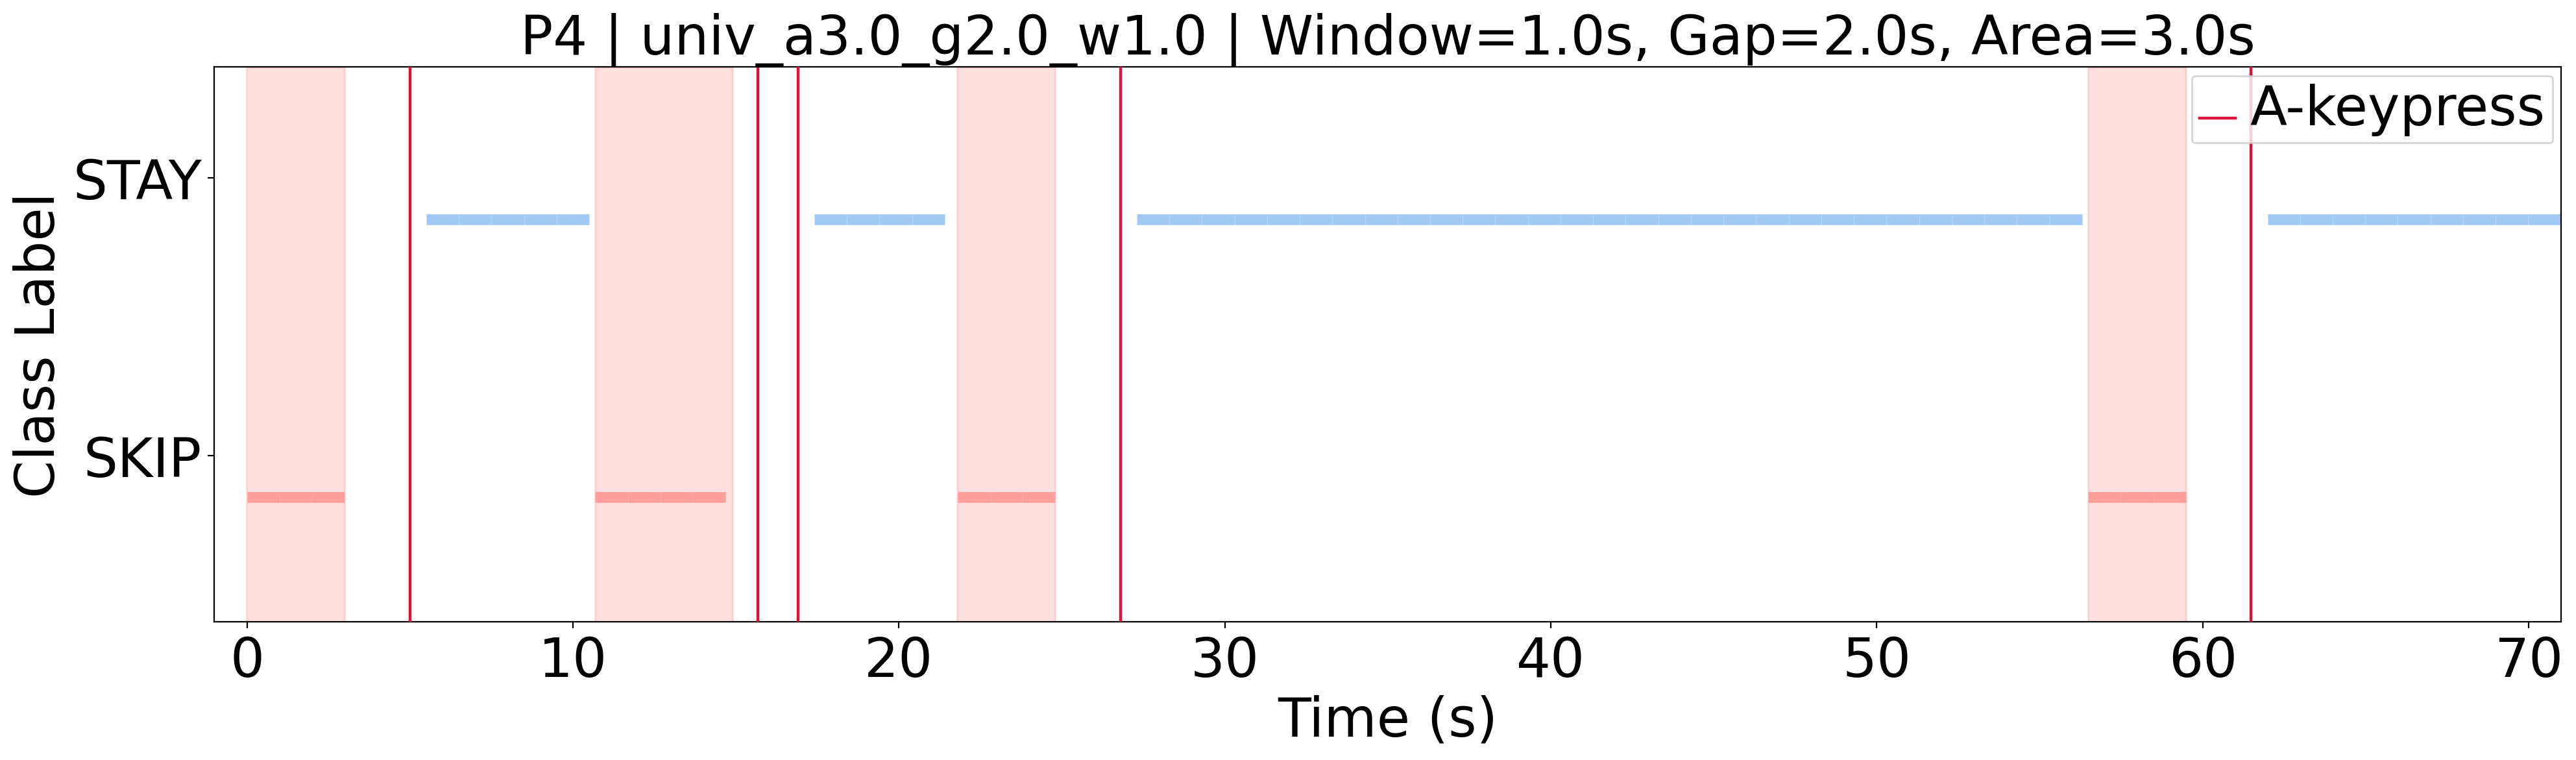
\includegraphics[width=\textwidth]{../05-12_data_analysis_and_results/runs/run_20260611_220844/viz/viz03_exploration/viz03_exploration_9.png}
    \caption{Schematic overview of the labeling strategy under the default parameterization. The figure illustrates the placement of the \texttt{STAY} and \texttt{SKIP} labels relative to the registered press markers, including the default gap length, window length, and imminent-skip period.}
    \label{fig:labeling_strategy}
\end{figure}

\subsection{Baseline Exclusion}
The manually categorized pre-task resting baseline phases were excluded from the \texttt{STAY}/\texttt{SKIP} classification dataset and used only for per-participant signal normalization. Consequently, the algorithms were trained to discriminate between active engagement (\texttt{STAY}) and approaching disengagement (\texttt{SKIP}) during browsing, rather than between resting and viewing. Figure~\ref{fig:labeling_strategy} illustrates the default labeling logic, including the press markers and the temporal placement of the labeling windows.

In addition to baseline exclusion, the labeling procedure omitted segments affected by boundary overlap between \texttt{STAY} and \texttt{SKIP} definitions. This was necessary to preserve clear class assignment and avoid ambiguous temporal regions near each swipe event. The final label construction therefore prioritized temporal purity of the target classes over maximal sample count.

\subsection{Parameter Sensitivity Analysis}

To assess how label definition affects class separability, a controlled sensitivity analysis over three temporal parameters was conducted. In each experiment, two parameters were held constant while the third was varied, isolating its effect. This setup allows us to distinguish whether separability is primarily driven by temporal distance to the swipe event, window size, or their interaction.

The influence of window size (ws), gap size (gs), and imminent-skip period (isp) on data preprocessing and segmentation is illustrated in three example-configurations: (i) default parameters (ws = 1s, gs = 2s, isp = 3s; Figure \ref{fig:labeling_strategy_default}), (ii) reduced window size (ws = 0.3s, gs = 2s, isp = 3s; Figure \ref{fig:labeling_strategy_small_window}), and (iii) reduced gap with extended imminent-skip period (ws = 1s, gs = 0.5s, isp = 4s; Figure \ref{fig:labeling_strategy_small_gap_big_isp}). The swipe event is indicated by vertical red lines. All figures show the same randomly selected 70-second segment from a single participant. Time (seconds) is plotted on the x-axis, and class labels—STAY (blue) and SKIP (red) on the y-axis.

\begin{figure}[H]
    \centering
    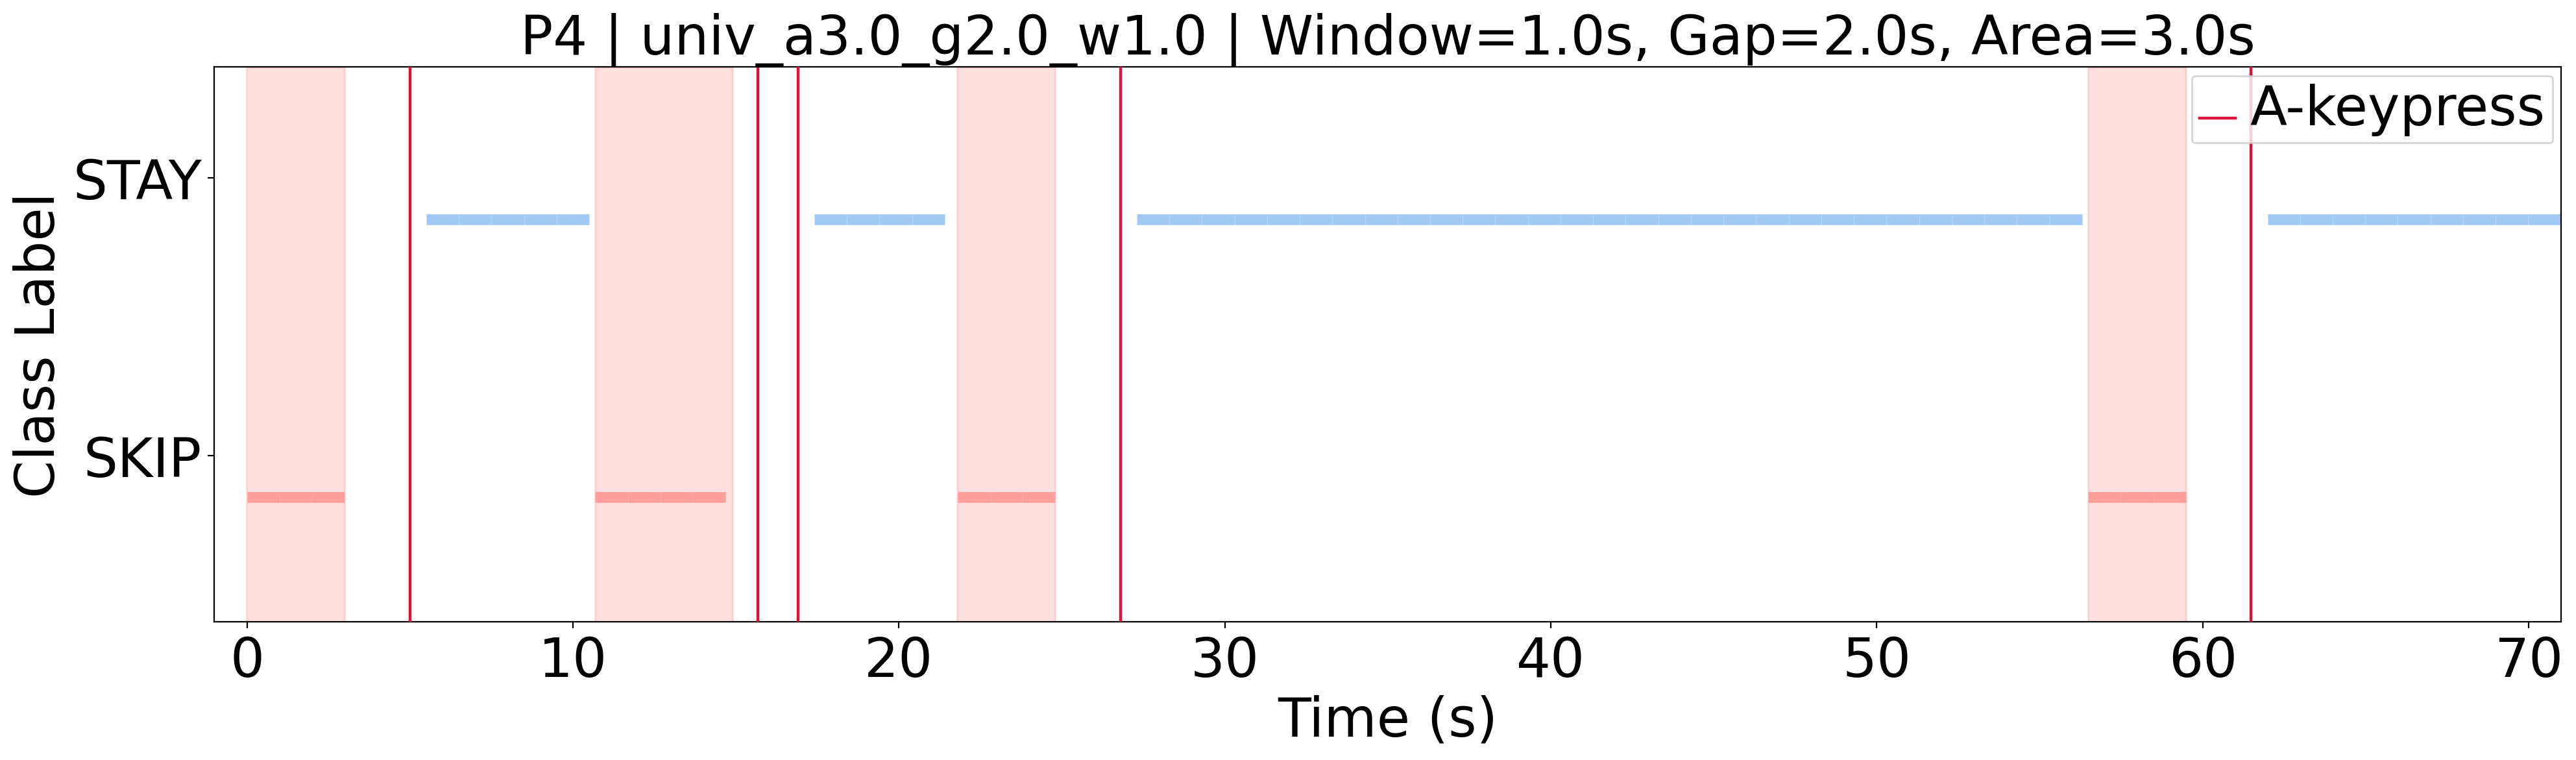
\includegraphics[width=\textwidth]{../05-12_data_analysis_and_results/runs/run_20260611_220844/viz/viz03_exploration/viz03_exploration_9.png}
    \caption{Window parameter exploration (default parameters, same as Figure \ref{fig:labeling_strategy}).}
    \label{fig:labeling_strategy_default}
\end{figure}

\begin{figure}[H]
    \centering
    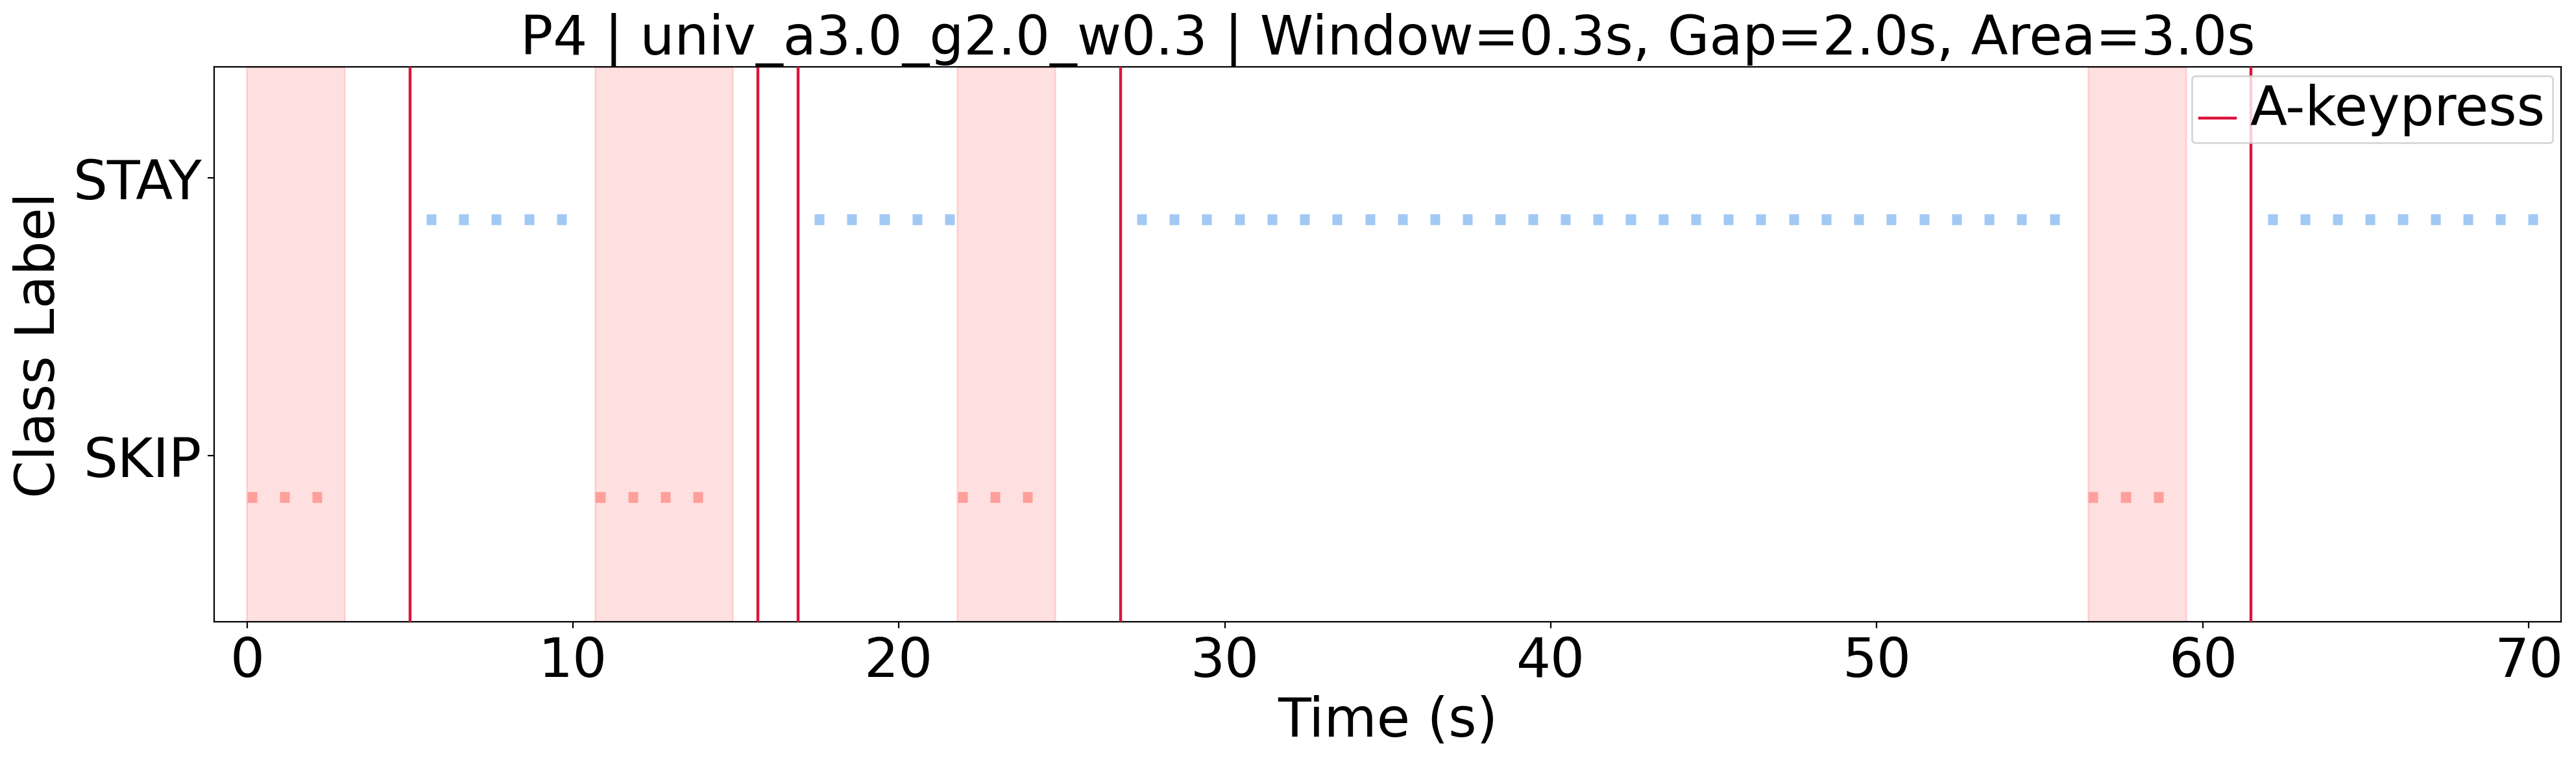
\includegraphics[width=\textwidth]{../05-12_data_analysis_and_results/runs/run_20260611_220844/viz/viz03_exploration/viz03_exploration_7.png}
    \caption{Window parameter exploration (default parameters, except a smaller window size).}
    \label{fig:labeling_strategy_small_window}
\end{figure}

\begin{figure}[H]
    \centering
    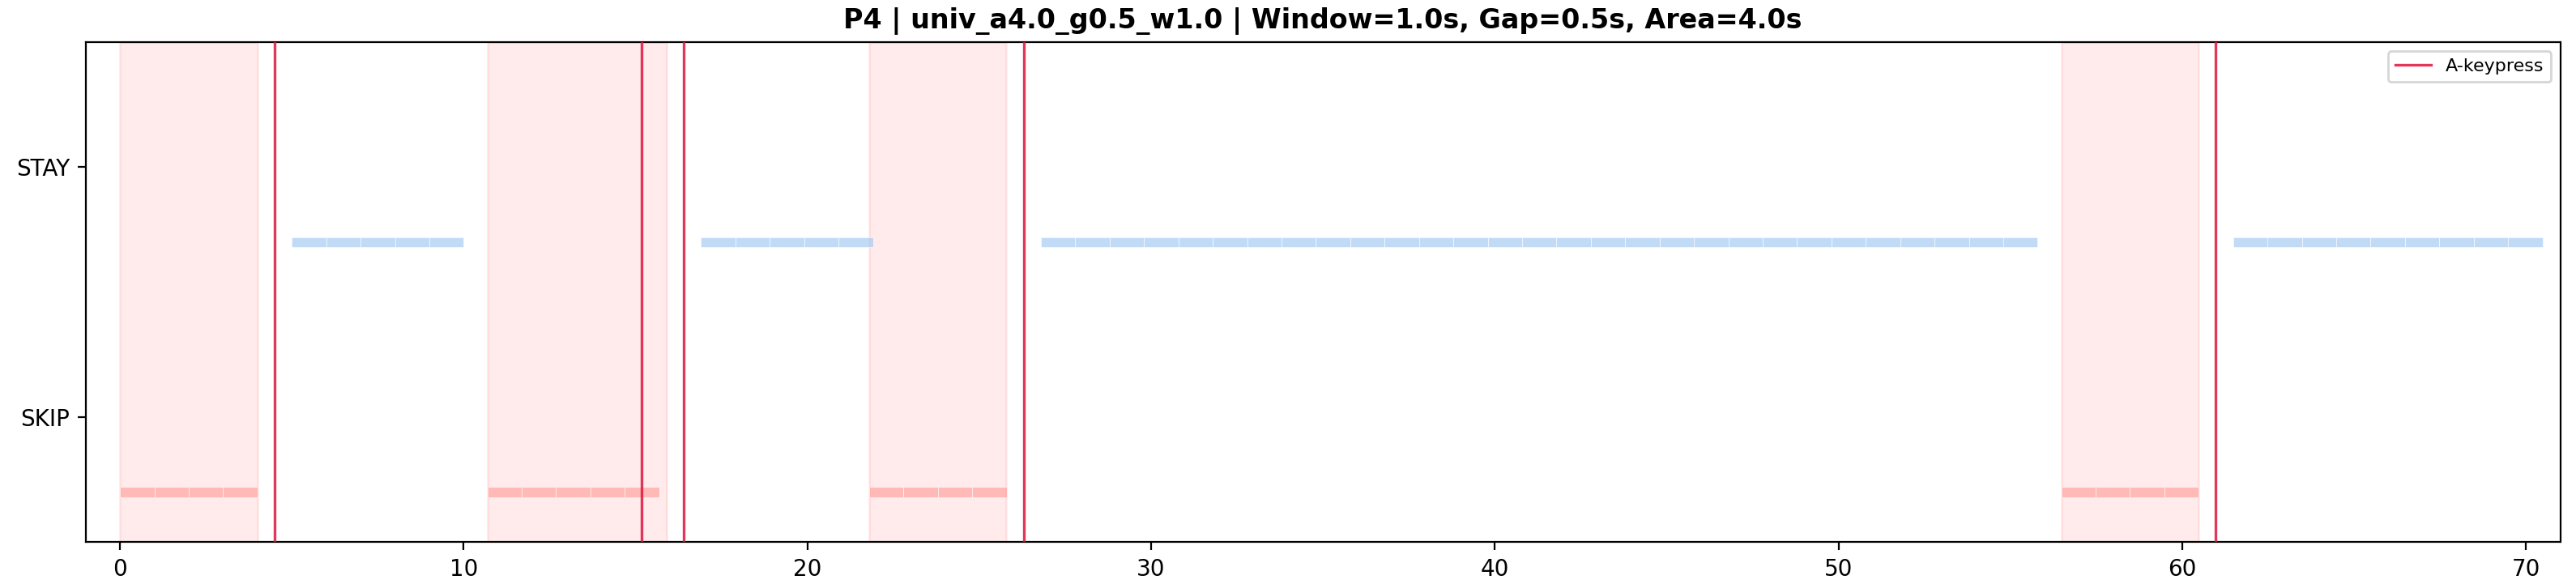
\includegraphics[width=\textwidth]{../05-12_data_analysis_and_results/runs/run_20260611_220844/viz/viz03_exploration/viz03_exploration_12.png}
    \caption{Window parameter exploration (default parameters, except a smaller gap size \& a longer imminent-skip period (Skip-Area)).}
    \label{fig:labeling_strategy_small_gap_big_isp}
\end{figure}

\begin{figure}[H]
    \centering
    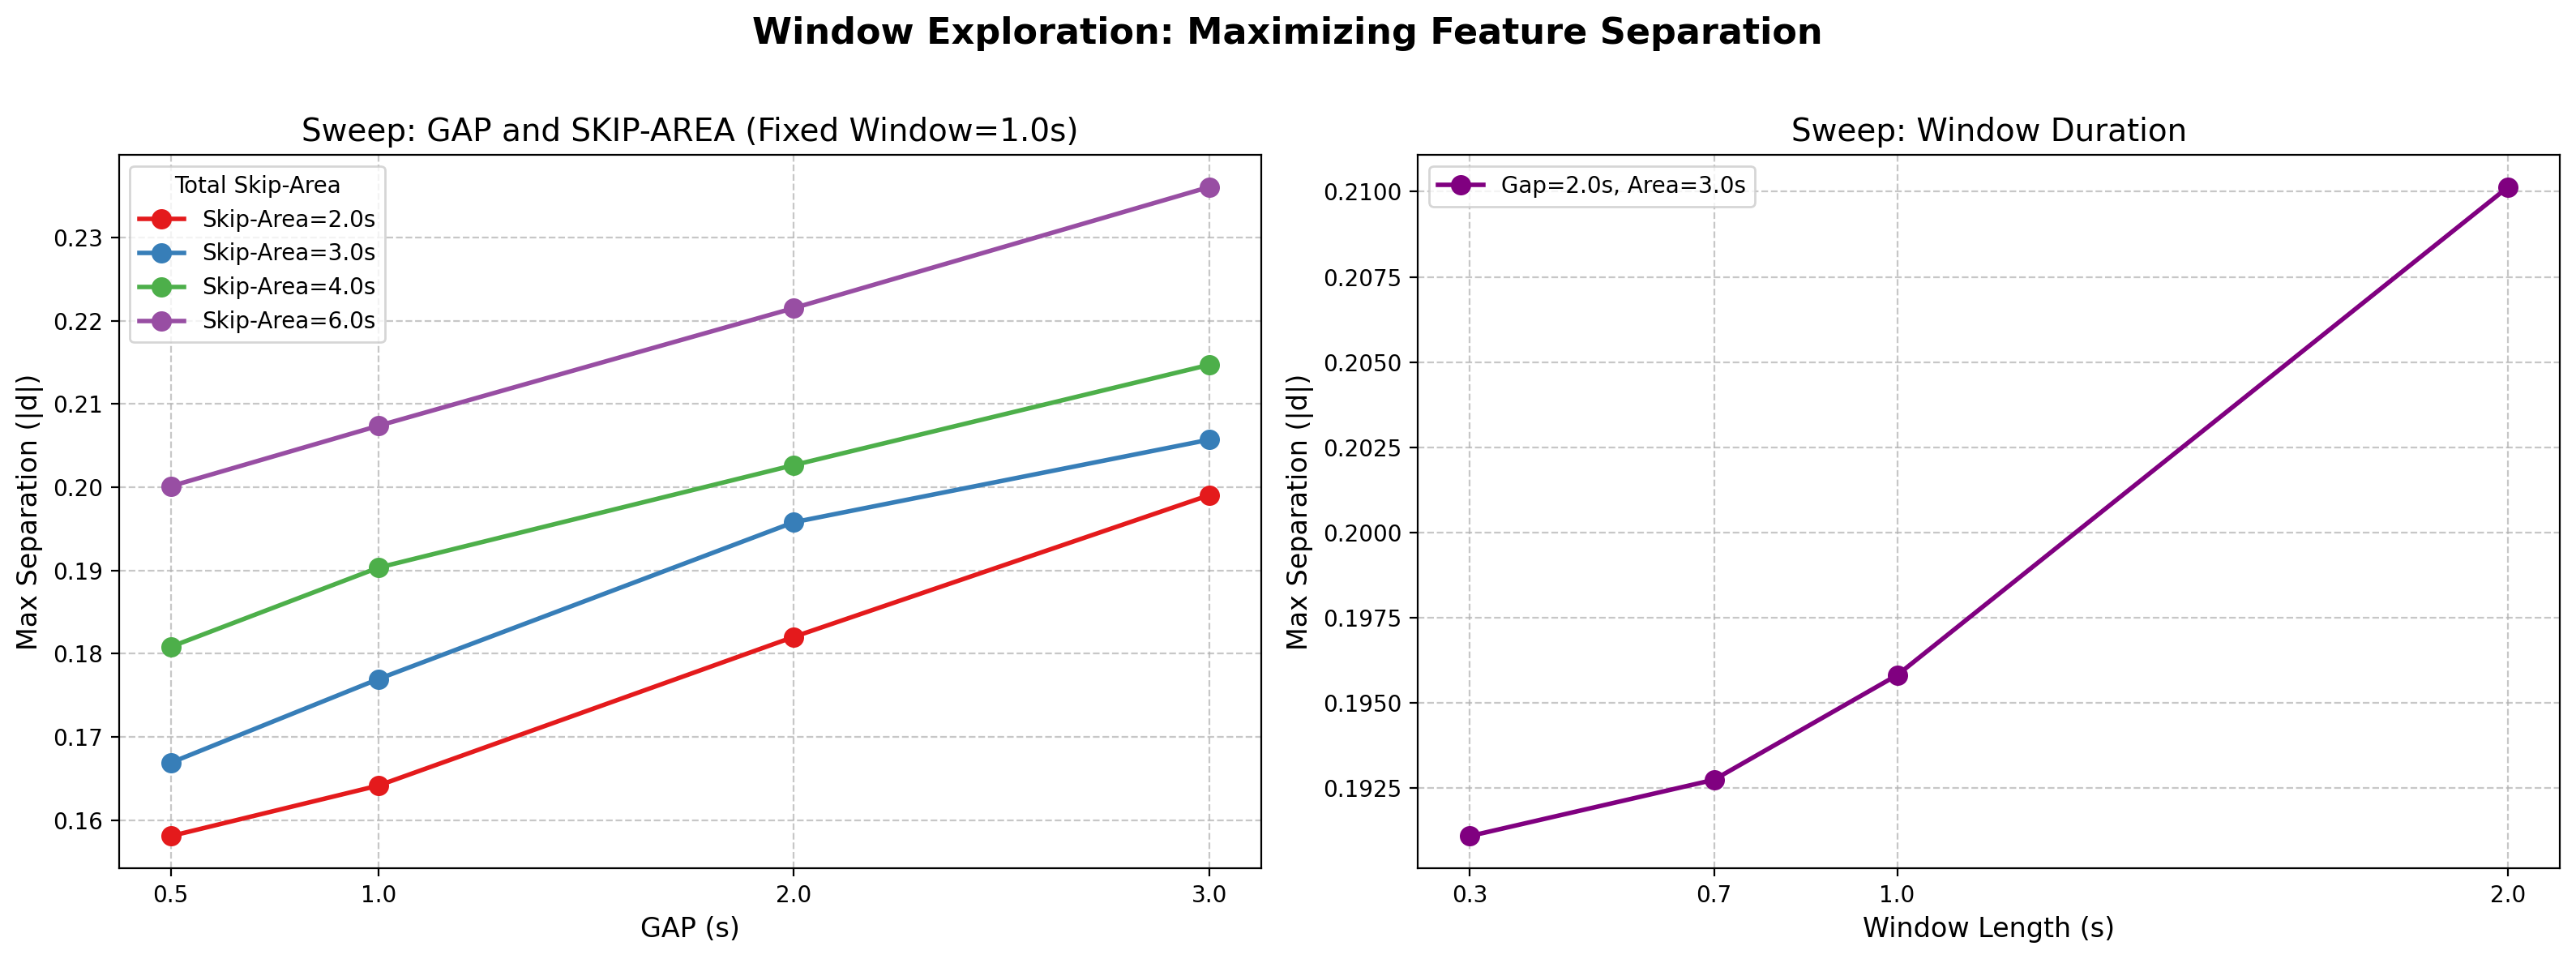
\includegraphics[width=\textwidth]{../05-12_data_analysis_and_results/runs/run_20260611_220844/viz/run_before_ei_fix/viz17_window_exploration_line.png}
    \caption{Parameter sweep of the window exploration analysis.}
    \label{fig:window_exploration}
\end{figure}

The key result is that, with fixed imminent-skip period and window size, increasing the gap length consistently increases Cohen’s d (Figure \ref{fig:window_exploration}, left), indicating greater separability as the SKIP interval moves further from the swipe event. A similar effect is observed for longer imminent-skip periods, where larger SKIP intervals also improve separability. For fixed gap and imminent-skip period, increasing window size shows a roughly linear or potentially cubic relationship with Cohen’s d (Figure \ref{fig:window_exploration}, right), again corresponding to increased class separation. While all these results strongly suggest better separability with increased overall data-availability (bigger windows, and areas) and simultaneously better separability the further we move away from the swipe, interpreting these relationships and their implications for optimal parameter selection remains beyond the scope of this thesis as it requires separate analysis, and is therefore a promising direction for future work. To maintain focus and scope, this analysis proceeds with the locked, default parameters:

\begin{itemize}
    \item Window size (ws) = 1 second
    \item Gap size (gs) = 2 seconds
    \item Imminent-skip period (isp) = 3 seconds
\end{itemize}

\subsection{Class Separation Metric}
\label{sec:method_class_separation_metric}
Cohen’s \(d\) was used as the primary descriptive measure of class separation. It expresses the standardized difference between the STAY and SKIP distributions, making it suitable for comparing separability across parameter settings even when the underlying distributions differ in scale. In this context, larger absolute values of Cohen’s \(d\) indicate stronger separation between the two classes.

\begin{equation}
    d = \frac{\bar{x}_{\text{STAY}} - \bar{x}_{\text{SKIP}}}{\sqrt{\frac{(n_{\text{STAY}} - 1)s_{\text{STAY}}^2 + (n_{\text{SKIP}} - 1)s_{\text{SKIP}}^2}{n_{\text{STAY}} + n_{\text{SKIP}} - 2}}}
    \label{eq:cohens_d}
\end{equation}
where \(\bar{x}_{\text{STAY}}\) and \(\bar{x}_{\text{SKIP}}\) denote the sample means of the feature values for the STAY and SKIP windows respectively, \(s_{\text{STAY}}^2\) and \(s_{\text{SKIP}}^2\) are the corresponding sample variances, and \(n_{\text{STAY}}\) and \(n_{\text{SKIP}}\) represent the number of samples in each class.

For each parameter configuration, Cohen’s \(d\) was computed between the STAY and SKIP feature distributions derived from the corresponding labeling scheme. This provided a direct quantitative index of how strongly the chosen temporal definitions emphasized the contrast between sustained engagement and imminent disengagement.

\section{Universal Recording Pipeline}
\label{sec:method_universal_recording_pipeline}
To facilitate rigorous and reproducible data collection, a robust Python-based recording architecture (\url{https://github.com/coffeeandcoffee/eeg_tiktok_pipeline/data_collection/recording_script.py}) was developed. This script orchestrates the simultaneous capture of raw EEG telemetry from the Muse S headband and has the capability of recording synchronized behavioral video from a webcam which was not used in this experiment, yet may be of value to future investigations. Its autonomous capabilities ensure that the experimental protocol can be executed reliably without extensive technical oversight.

For this study's recordings the command \verb|python recording_script_v4.py --nocamera --duration 1800| was used to call the script. The two flags simply mean (i) bypassing camera recording, as it is not in the scope of this study yet kept for future investigations and (ii) the recording duration is 1800s = 30 minutes.
The pipeline's core features include:
\begin{itemize}
    \item \textbf{Automated Hardware Discovery:} Upon launch, the script automatically scans the local Bluetooth environment for active Muse devices and enumerates all connected camera peripherals, allowing the researcher to select the optimal hardware interactively without requiring hardcoded MAC addresses or device indices.
    \item \textbf{Precision Synchronization and Event Logging:} A dedicated, threaded keypress listener (\texttt{pynput}) monitors the \texttt{A} and \texttt{B} keys used by participants to mark swipe events and baseline respectively. Crucially, the script computes a dynamic time offset between the system clock and the LSL stream clock. Keypresses are retroactively aligned to this LSL timeline within a defined tolerance window and embedded directly into the EEG data rows as binary flags, ensuring absolute temporal synchrony between cognitive events and physical interactions.
    \item \textbf{Simultaneous Multimodal Capture:} The script utilizes the \texttt{pylsl} library to interface with the Lab Streaming Layer (LSL), pulling raw EEG data from the Muse headband at 256 Hz. Unless deactivated with the flag, it concurrently employs OpenCV to capture and encode synchronized webcam video using the H.264 (avc1) codec, providing visual ground truth of participant behavior.
    \item \textbf{Resilient Auto-Reconnection:} To combat the inherently unstable nature of Bluetooth Low Energy (BLE) connections, the script features an active connection-loss detection loop. If the LSL stream halts (no samples received within a timeout period), the script automatically terminates the hanging subprocess, rescans the Bluetooth environment, restarts the stream, and initiates a sequential data fragment (e.g., \verb|_2.csv|, \verb|_3.csv|). This guarantees that transient connection drops do not corrupt the entire recording session.
    \item \textbf{Concurrent Multi-Threading:} To ensure that blocking operations (such as writing high-resolution video frames to disk) do not disrupt the high-frequency polling required for EEG telemetry, the script isolates the LSL pulling loop, the OpenCV capture loop, and the keypress listener into independent Python daemon threads.
\end{itemize}

This open-source compatible architecture ensures that any independent researcher equipped with a standard webcam and a consumer-grade Muse S headband can fully replicate the data collection methodology utilized in this thesis.

\section{Universal Pre-Processing Pipeline}
\label{sec:method_universal_preprocessing_pipeline}

The following subsections describe step-by-step exactly what the Python code in the \url{https://github.com/coffeeandcoffee/eeg_tiktok_pipeline} directory executes to process the raw EEG signals into a uniform shape suitable for analysis.

\subsection{Data Synchronization and Interpolation}
The preprocessing pipeline began with the chronological alignment and concatenation of all recorded CSV files for each participant, ensuring a continuous temporal sequence (executed via \url{https://github.com/coffeeandcoffee/eeg_tiktok_pipeline/data_analysis/step01_preprocess.py}). The raw data streams collected from the LSL (Lab Streaming Layer) exhibited slight variations in intrinsic sampling rates. To establish a uniform temporal grid suitable for across-session and across-participant analysis, the true sampling rate was derived by calculating the median time difference (\(\Delta t\)) between consecutive timestamps. Subsequently, a linear interpolation algorithm was applied to upsample and regularize the data to a constant sampling frequency of exactly \(f_s = 256\) Hz. This process guarantees that any subsequent spectral analysis relies on a strictly uniform time axis, avoiding mathematical artifacts stemming from temporal jitter.

% this is just to demonstrate that after interpolation all are 256Hz exactly, which is nessecary for the data to be used properly for processing and analysis
\begin{figure}[H]
    \centering
    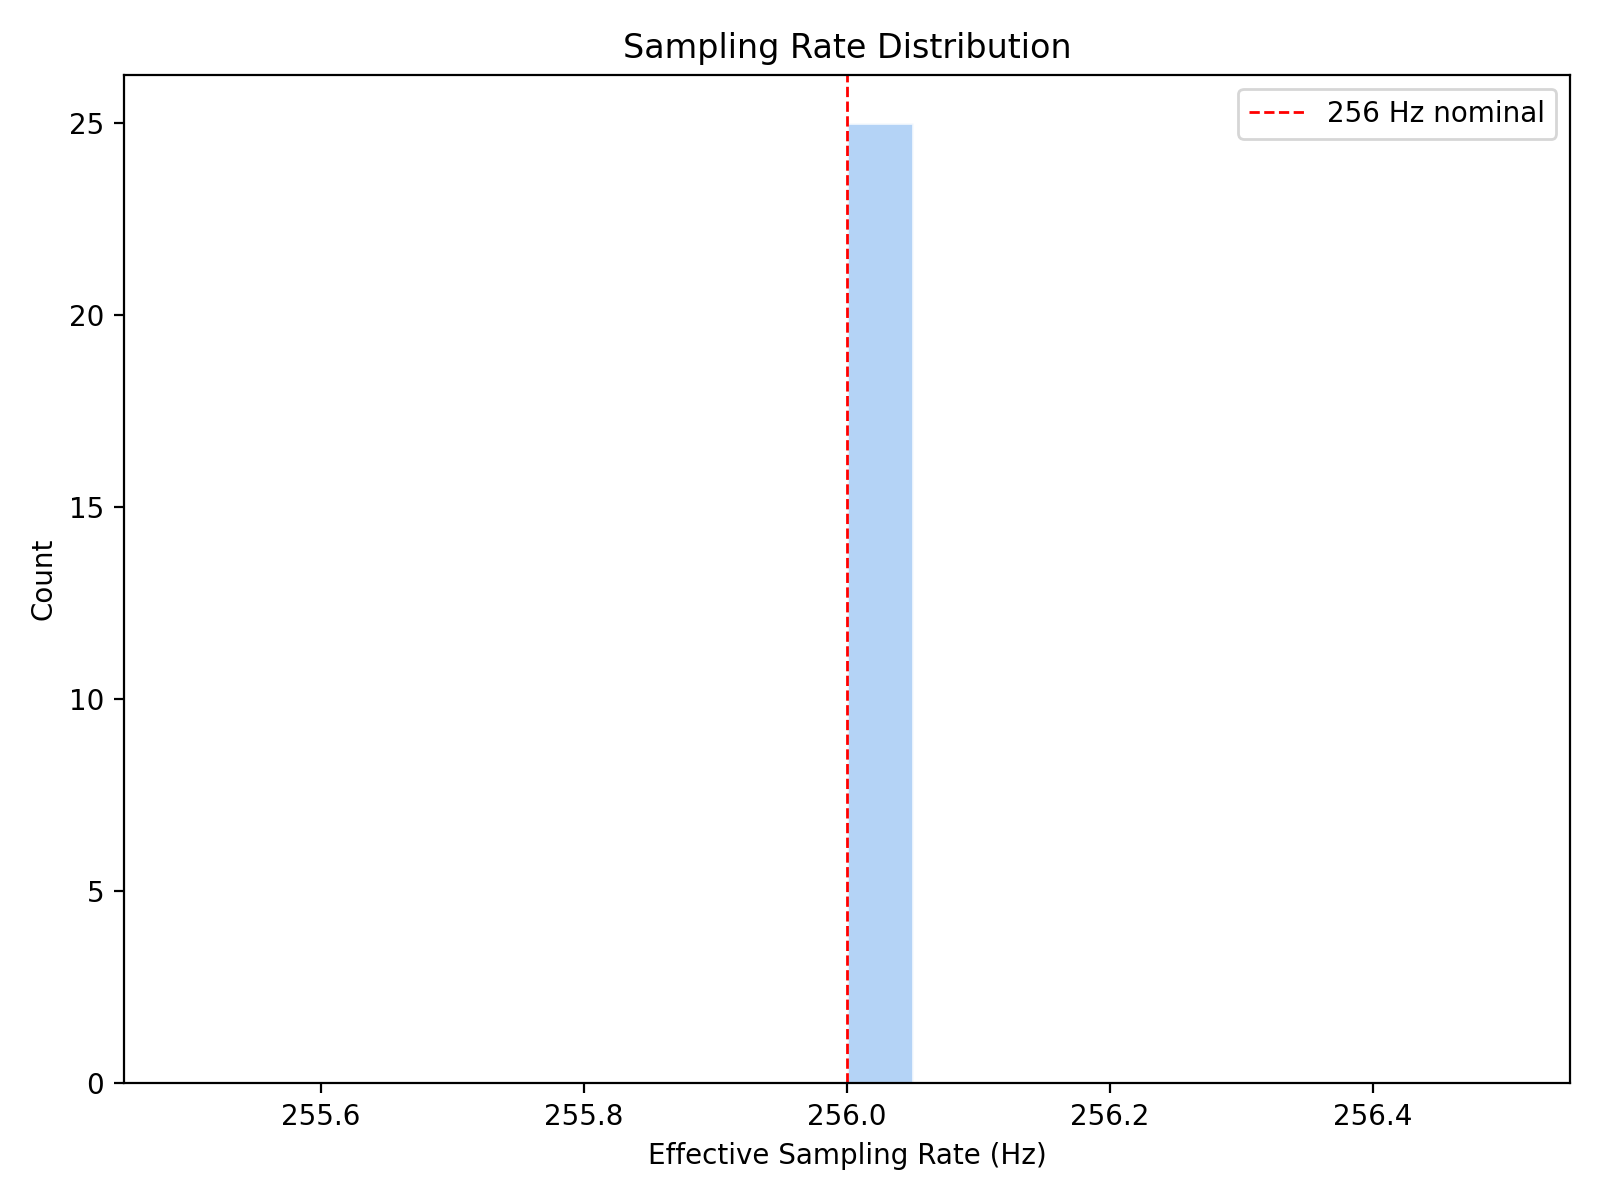
\includegraphics[width=\textwidth]{../05-12_data_analysis_and_results/runs/run_20260611_220844/viz/viz01.1.png}
    \caption{Sampling Rate Distribution across participants, demonstrating that after interpolation all signals operate precisely at 256 Hz, which is a mathematical prerequisite for the correct extraction of spectral band power.}
\end{figure}

During this temporal alignment process, Bluetooth transmission dropouts were identified by locating unnatural temporal gaps between consecutive CSV boundaries. To ensure data integrity, the duration of these dropouts was logged, and any potential data windows traversing such boundaries were strictly excluded in later extraction phases.

% this just shows that bluetooth dropouts happened but are not very many, and we handle them appropriately by eliminating any STAY or SKIP area that is touched by such an event.
\begin{figure}[H]
    \centering
    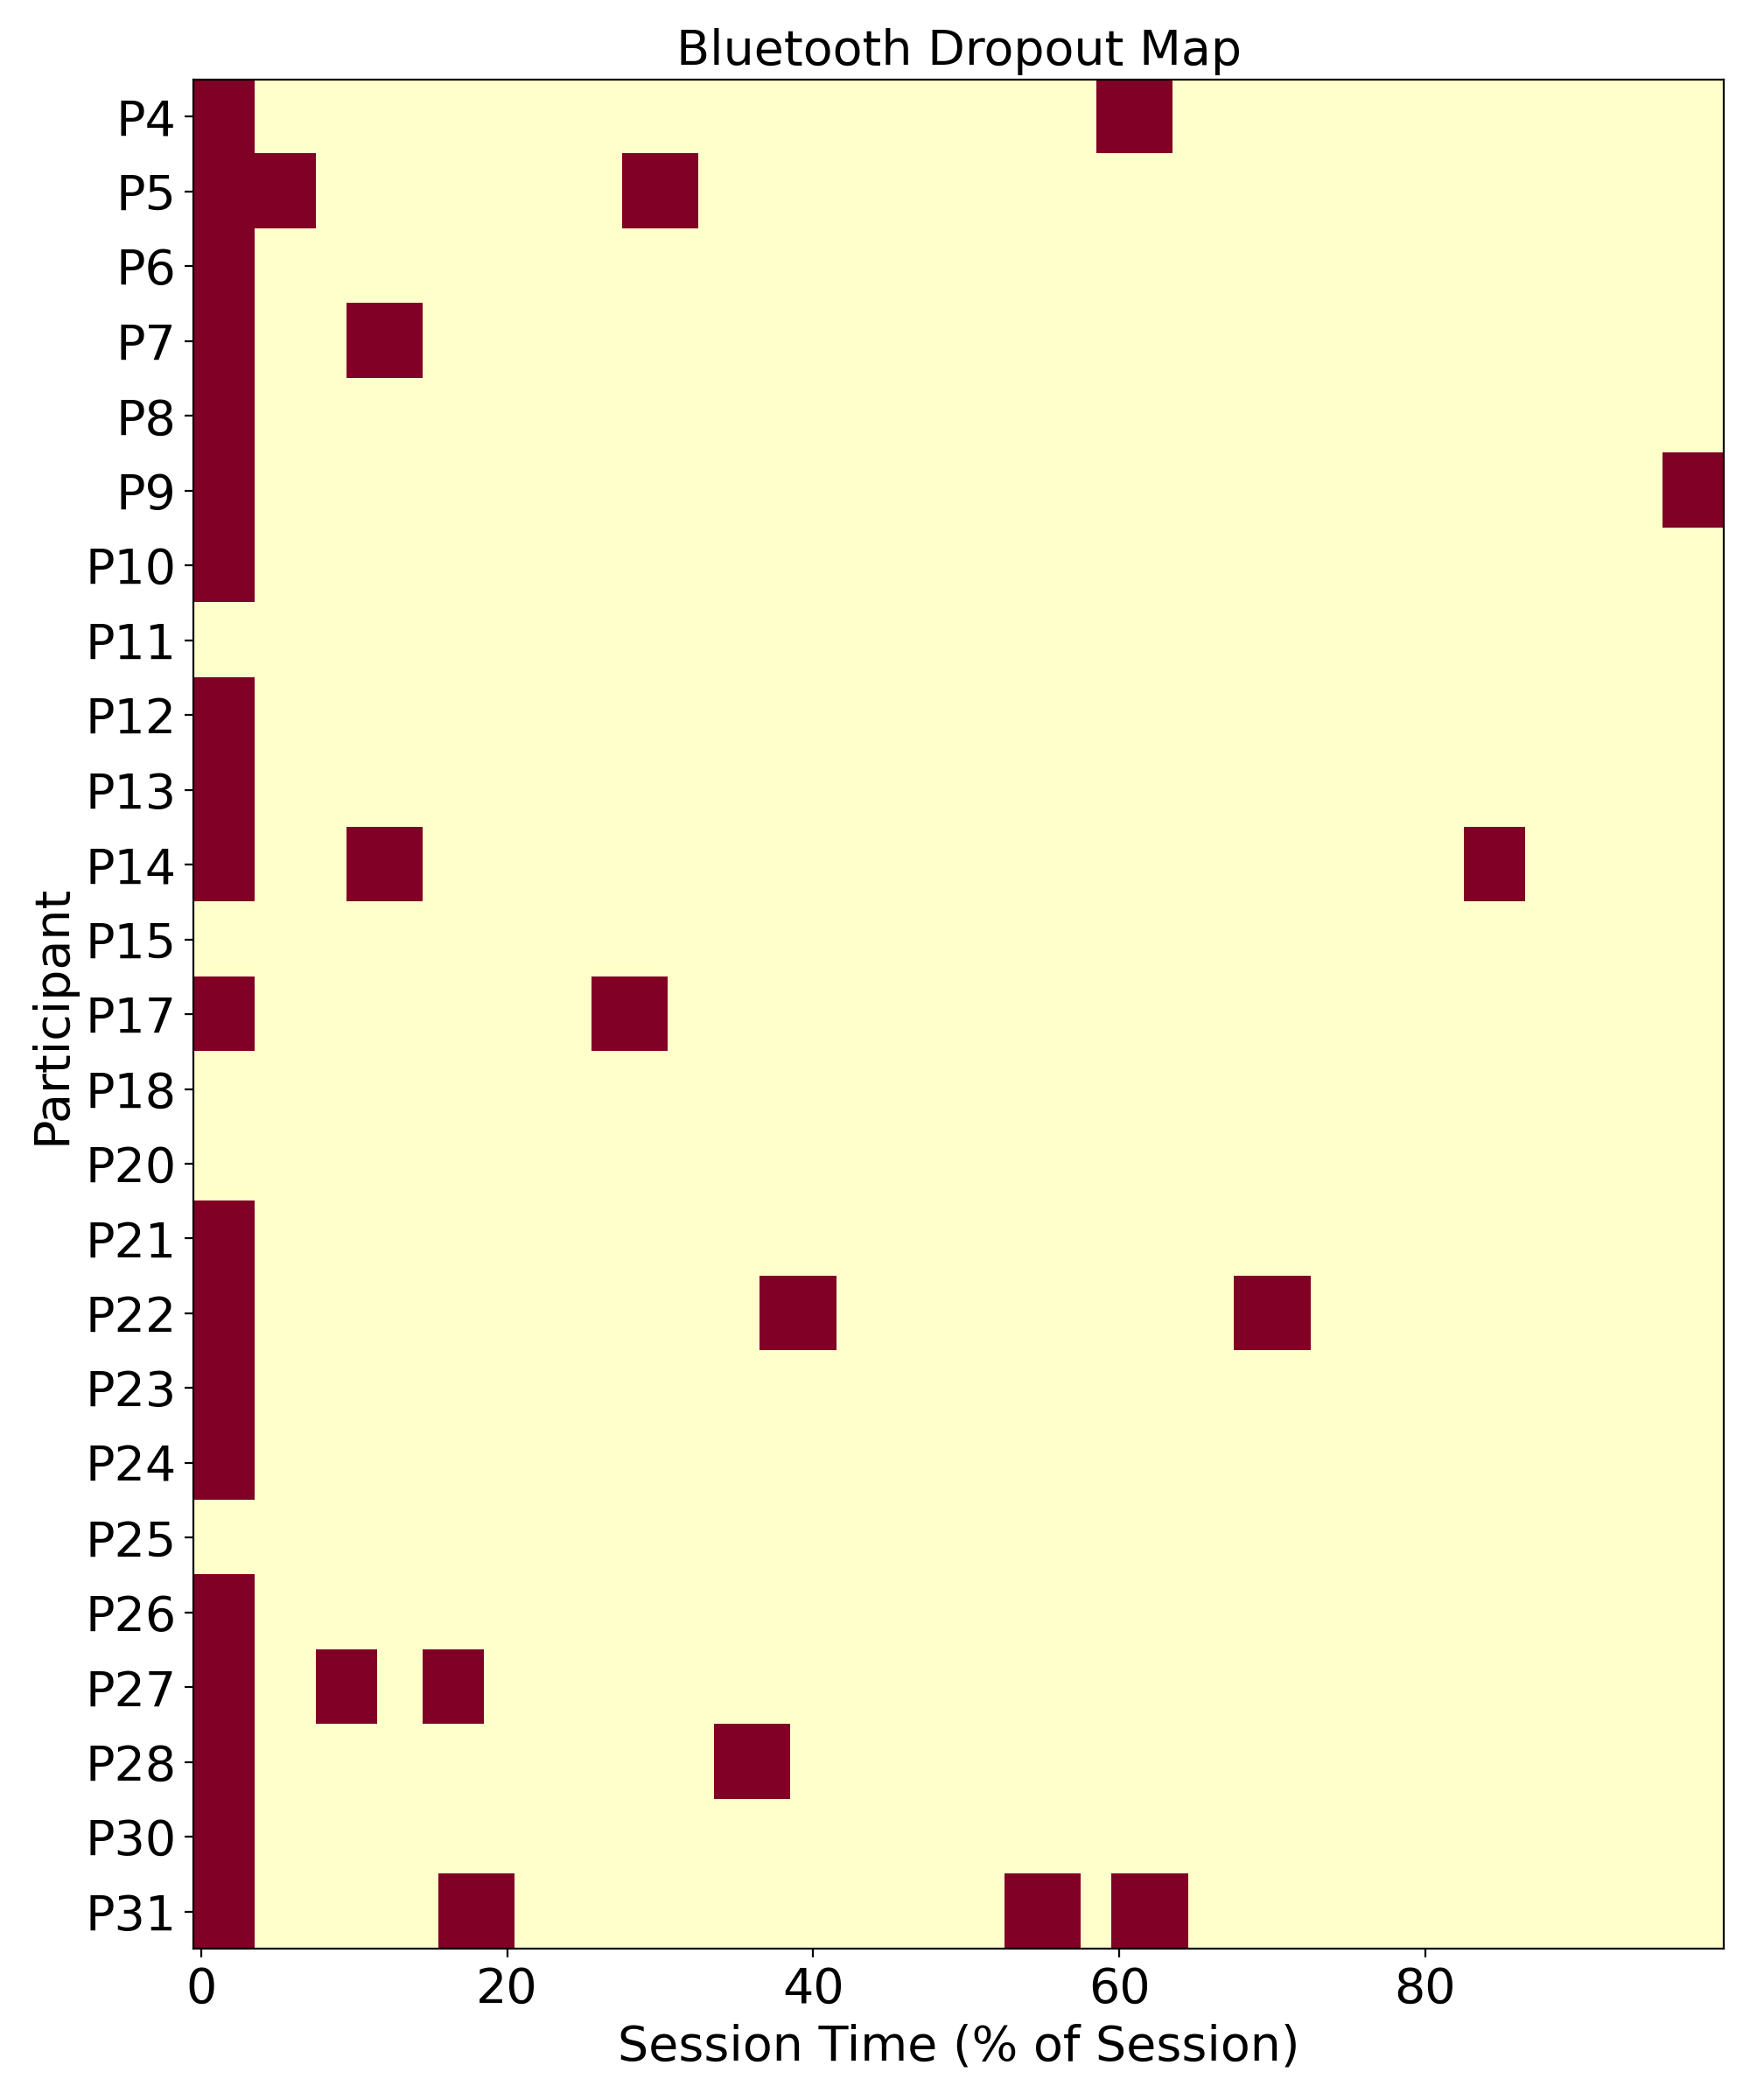
\includegraphics[width=\textwidth]{../05-12_data_analysis_and_results/runs/run_20260611_220844/viz/viz01.3.png}
    \caption{Bluetooth Dropout Heatmap indicating signal loss events across the experimental timeline. Data windows overlapping with these dropouts were removed from the analysis pipeline.}
\end{figure}

\subsection{Baseline Extraction and Normalization}
Following temporal synchronization, a baseline resting state was extracted for each participant to account for individual physiological differences, such as varying skull thickness or inherent resting cortical activity. The baseline period was rigidly defined as a 90-second continuous window commencing 10 seconds after the participant's initial \texttt{B} keypress (executed via \url{https://github.com/coffeeandcoffee/eeg_tiktok_pipeline/data_analysis/step01_preprocess.py}). 

The interpolated signal was then separated into seven standard EEG frequency bands (Delta, Theta, Alpha, Beta, Low Gamma, High Gamma, and Very High Gamma) utilizing a 4th-order Butterworth bandpass filter. The instantaneous amplitude envelope for each band was extracted and squared to compute the instantaneous spectral power \(P\). 

To normalize the extracted features across participants, a z-score relative power normalization was applied against the participant-specific baseline. For every temporal sample, the normalized spectral power \(z\) was computed as:
\begin{equation}
    z = \frac{P - \mu_{base}}{\sigma_{base}}
\end{equation}
where \(\mu_{base}\) and \(\sigma_{base}\) denote the mean and standard deviation of the spectral power derived exclusively from the aforementioned 90-second baseline period. This relative power transformation ensures that all subsequent statistical evaluations and machine learning models operate on normalized deviations from a participant's own resting state, effectively mitigating absolute inter-subject voltage variance.

\subsection{Windowing and Class Labeling}
Following normalization, the continuous data streams were segmented and labeled into discrete \texttt{STAY} and \texttt{SKIP} classes based on the participant's interaction events (\texttt{A} keypresses) as previously established in Sections~\ref{sec:op_labeling_params} and \ref{sec:op_stay_skip}. To strictly prevent motor artifact contamination arising from the physical swipe action, a \textbf{2.0-second gap} was enforced immediately preceding the \texttt{A} keypress, and a \textbf{0.5-second gap} was enforced immediately following it. No data was extracted from these gap periods.

The \texttt{SKIP} class was rigorously defined as the \textbf{3.0-second window} immediately preceding the aforementioned 2.0-second pre-swipe gap (executed via \url{https://github.com/coffeeandcoffee/eeg_tiktok_pipeline/data_analysis/step03_label_windows.py}). This temporal framing specifically isolates the critical cognitive decision-making phase leading up to the swipe, entirely uncontaminated by the physical execution of the swipe itself. The \texttt{STAY} class was defined as all remaining valid temporal periods outside of the \texttt{SKIP} windows and safety gaps.

Finally, discrete 1.0-second analysis windows were extracted using a sliding window with no overlap (stride = window length). This ensures that windows do not cross class boundaries, enter safety gaps, or overlap with adjacent samples, thereby preventing data leakage and artificially inflated model performance.

\subsection{Artifact Analysis}
To ensure the integrity of the analyzed EEG signals, an automated outlier detection approach was implemented to flag potential artifacts (executed via \url{https://github.com/coffeeandcoffee/eeg_tiktok_pipeline/data_analysis/step02_artifact_flag.py}). Specifically, the 95th percentile of the peak-to-peak amplitude computed on the notch-filtered signal was utilized as a dynamic, participant-specific threshold. Frontal channels (AF7, AF8) were evaluated for ocular artifacts (e.g., blinks), while temporal channels (TP9, TP10) were evaluated for electromyogenic (EMG) artifacts. Absolute voltage thresholds (e.g., \(150\mu V\)) were initially investigated but were ultimately discarded as they did not yield generalizable or useful results across the dataset.

No data points were excluded from the final machine learning pipeline based on these artifact flags. Incorporating such filtering would introduce additional experimental conditions and substantially expand the analysis beyond the scope of this proof-of-concept study. Instead, the approach is documented to highlight awareness of artifact-related confounds and to provide a foundation for more advanced rejection strategies in future work.

% this is not used in results, and is more informaive, that this is more to show that we thought about this: that this is how artifact rejection could be done defining a percentile of outliers, but may require more sophisticated algorithm - but this is not part of the scope of this thesis as it is only proof of concept for distinguidhing the classes from EEG, thats why it will continute without artifact rejection and this is a great further direction of investigation.
\begin{figure}[H]
    \centering
    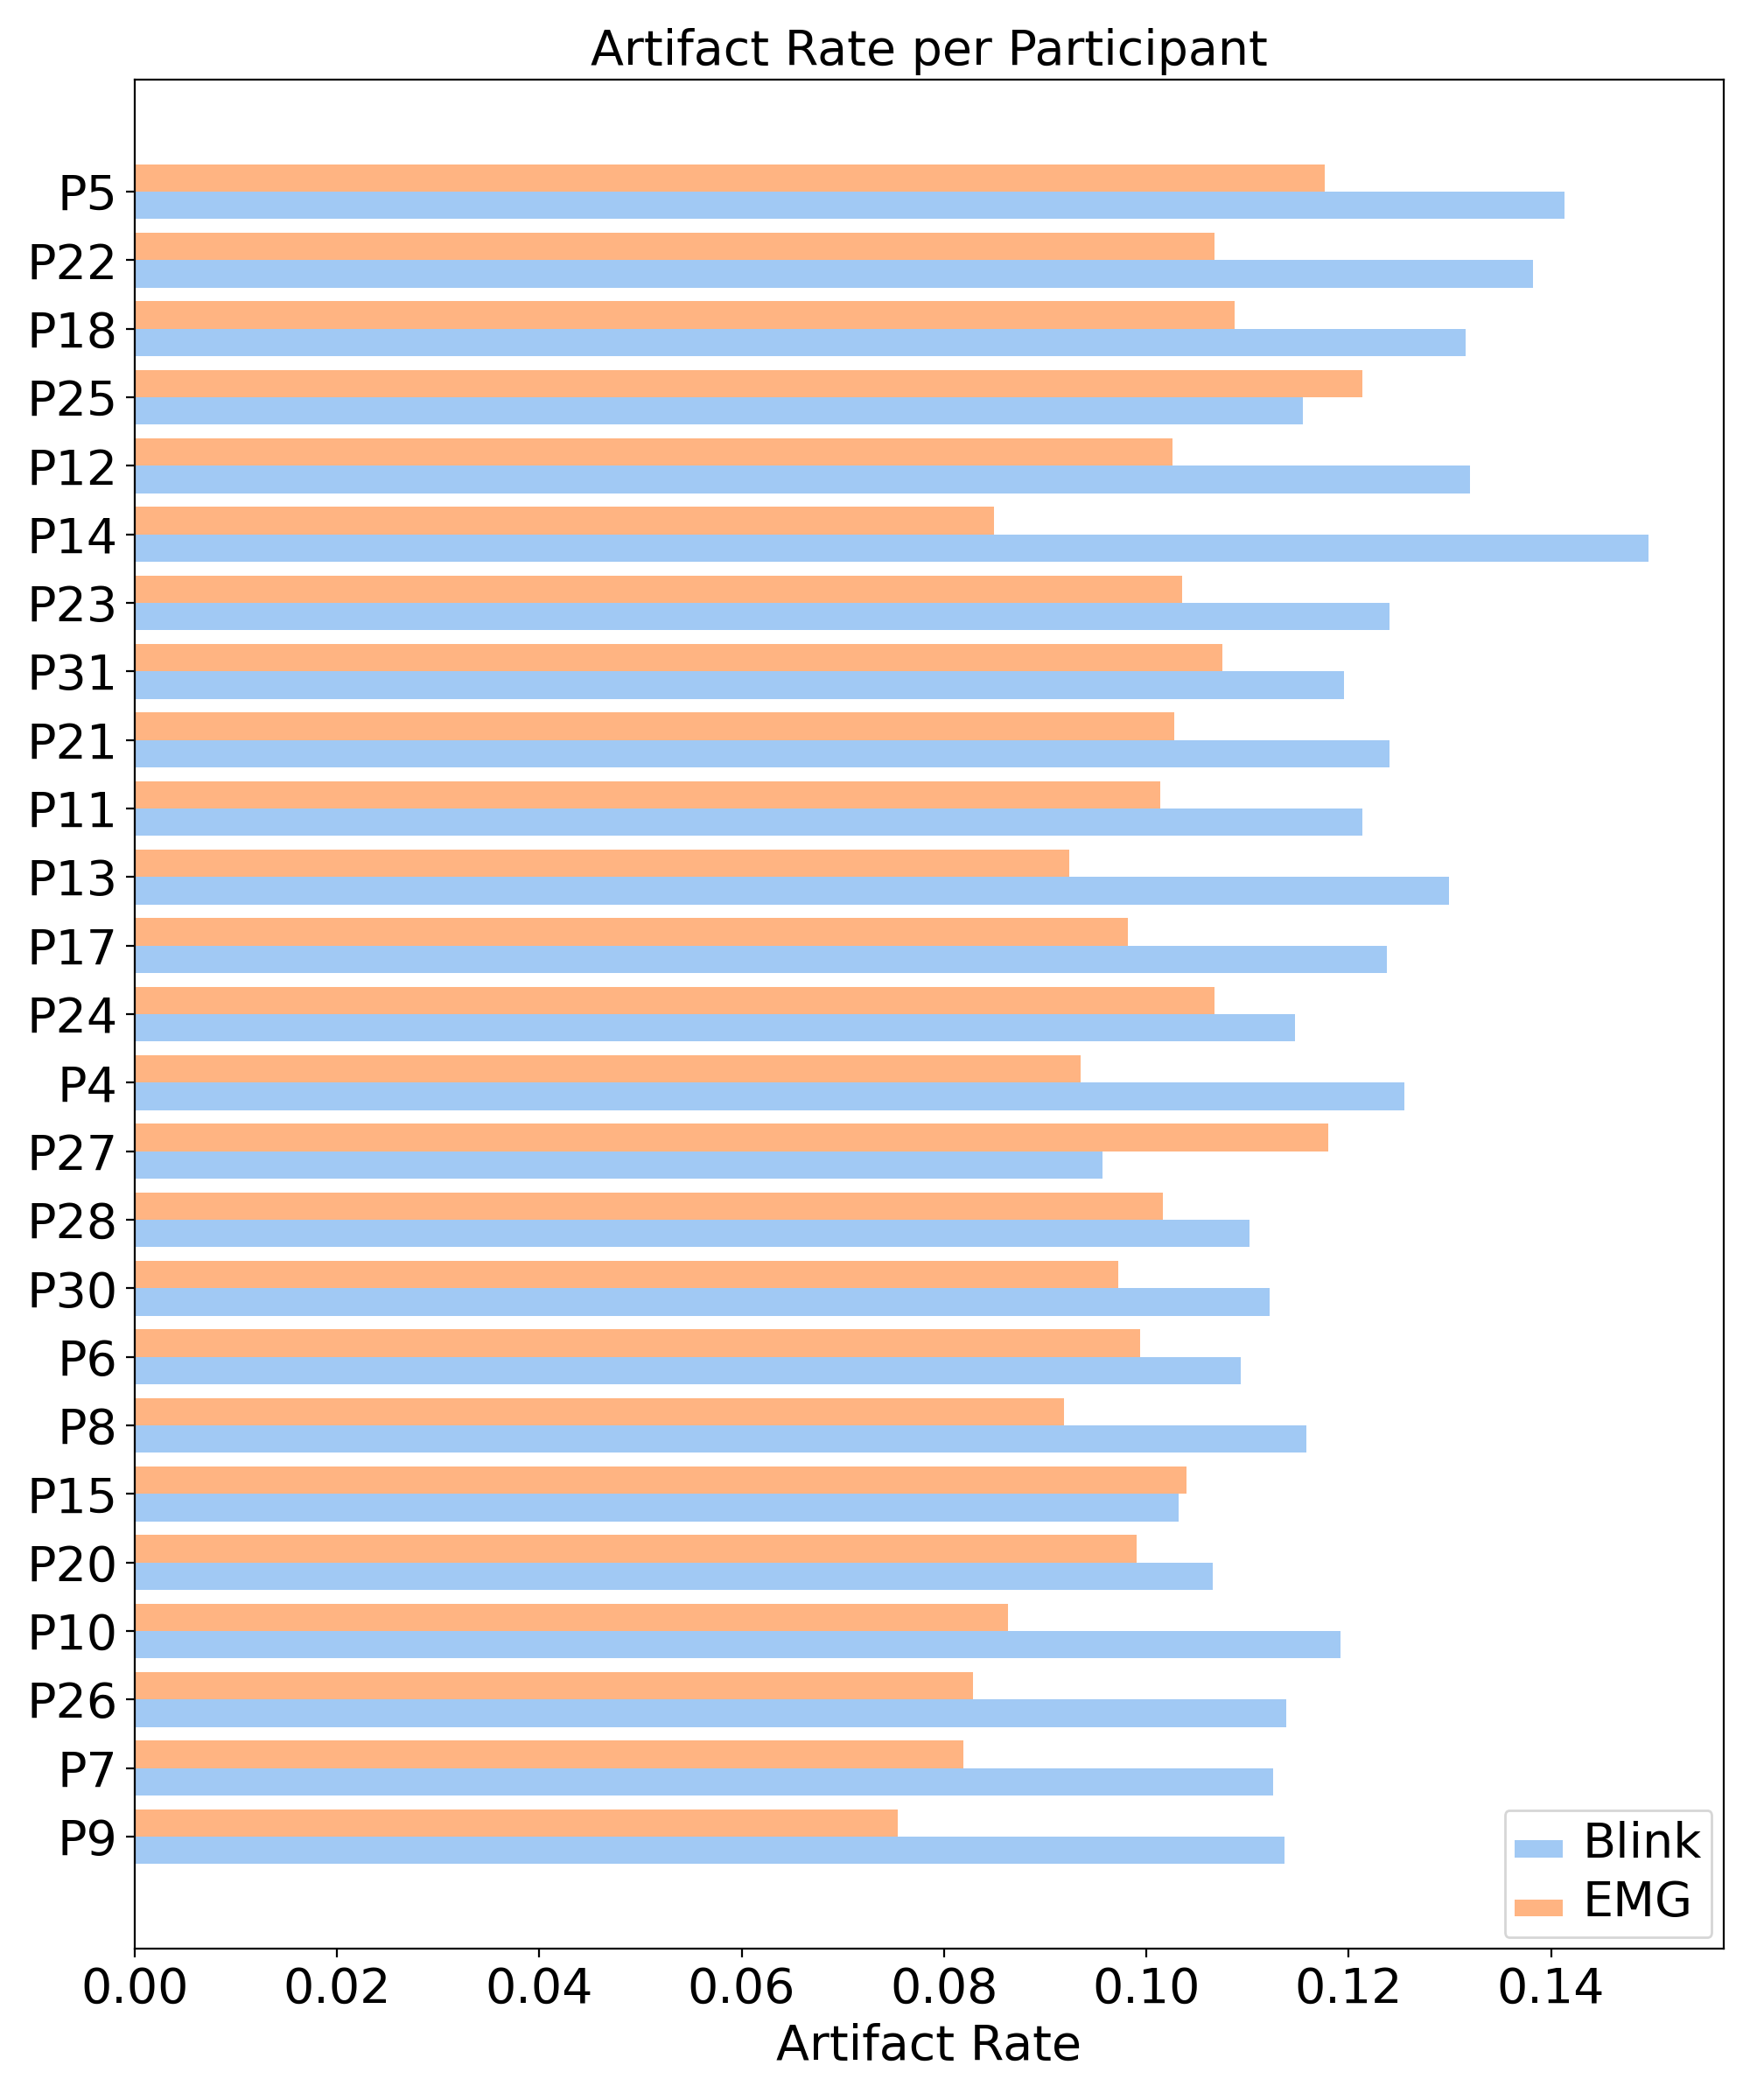
\includegraphics[width=\textwidth]{../05-12_data_analysis_and_results/runs/run_20260611_220844/viz/viz02.1.png}
    \caption{Artifact rate distribution and signal quality flagging based on the 95th percentile peak-to-peak outlier approach.}
\end{figure}

\subsection{Behavioral Burst Analysis}
\label{sec:method_behavioral_burst_analysis}

In addition to physiological artifacts, behavioral anomalies termed “bursts” were identified. A burst is defined as a sequence of rapidly successive skip events (e.g., multiple \texttt{A} keypresses merging into a single contiguous temporal block), reflecting frantic swiping rather than deliberate evaluation. Flagging these events aims to ensure that the \texttt{SKIP} class captures genuine cognitive disengagement rather than high-momentum, low-engagement scrolling behavior.

Although bursts were successfully detected, they were not excluded from the final analysis. Figure~\ref{fig:bursts} visualizes the detection mechanism via the distribution of inter-swipe intervals (i.e., dwell time) across all participants. The vertical threshold marks the 6.0-second merge boundary (2×the 3.0-second \texttt{SKIP} window). Consecutive swipes below this threshold cause their respective \texttt{SKIP} windows to overlap and merge into a single contiguous block, thereby defining a burst. The shaded region highlights the frequency of such rapid, consecutive events.

It is important to note that the \texttt{SKIP} window size is defined independently of the dwell time distribution; the 3.0-second value is an intuitive choice. As such, its influence on the resulting burst structure warrants further investigation. Incorporating burst rejection would introduce additional analytical complexity and is therefore beyond the scope of this proof-of-concept study. Instead, its inclusion highlights a relevant behavioral confound and motivates future work.

% this is not used in results, and is more informaive, that this is more to show that we thought about this: that is how many times people swipe in a row - which we call in this thesis 'Bursts' - and it is another viable parameter and direction of investigation that is interesting for future work beyond this thesis, as again the focus is another.
\begin{figure}[H]
    \centering
    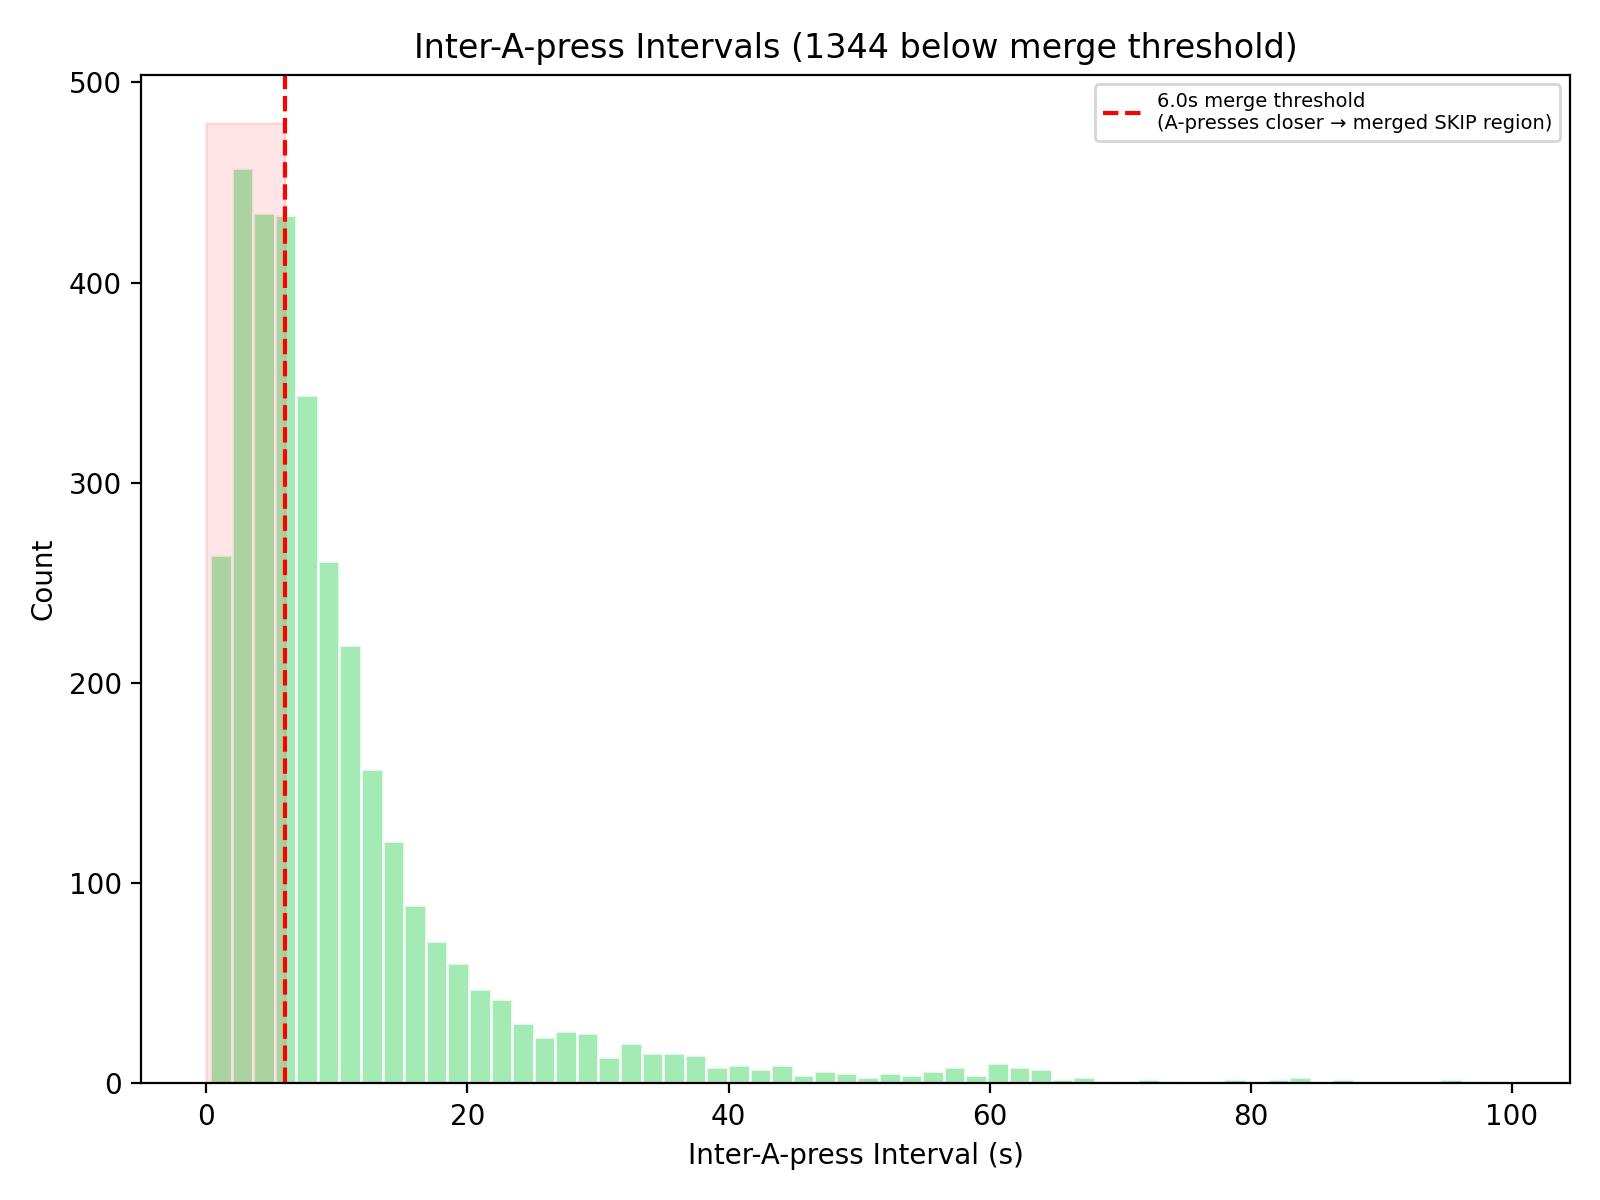
\includegraphics[width=\textwidth]{../05-12_data_analysis_and_results/runs/run_20260611_220844/viz/viz03/viz03.3.png}
    \caption{Distribution of inter-swipe intervals (view times of each video across all participants, or dwell time). The shaded region highlights intervals below the 6.0-second merge threshold, where consecutive \texttt{SKIP} windows overlap to form behavioral burst blocks.}
    \label{fig:bursts}
\end{figure}

\section{Feature Engineering}
\label{sec:method_feature_engineering}

\subsection{Band Power and Statistical Moments}
Following window extraction, a comprehensive feature set was computed for each valid temporal window (executed via \url{https://github.com/coffeeandcoffee/eeg_tiktok_pipeline/data_analysis/step05_feature_engineering.py}). For each of the 4 electrodes across the 7 previously defined frequency bands, four primary statistical moments were extracted: Mean, Standard Deviation, Minimum, and Maximum. An example of these extracted statistical moments belonging to one temporal 1-second window of one frequency band (alpha) of one electrode of one participant, is depicted in Figure~\ref{fig:stat_moments}.

% for explanation of each statistical moment definition and exact calculation, and dimension, and how it differs from EI
\begin{figure}[H]
    \centering
    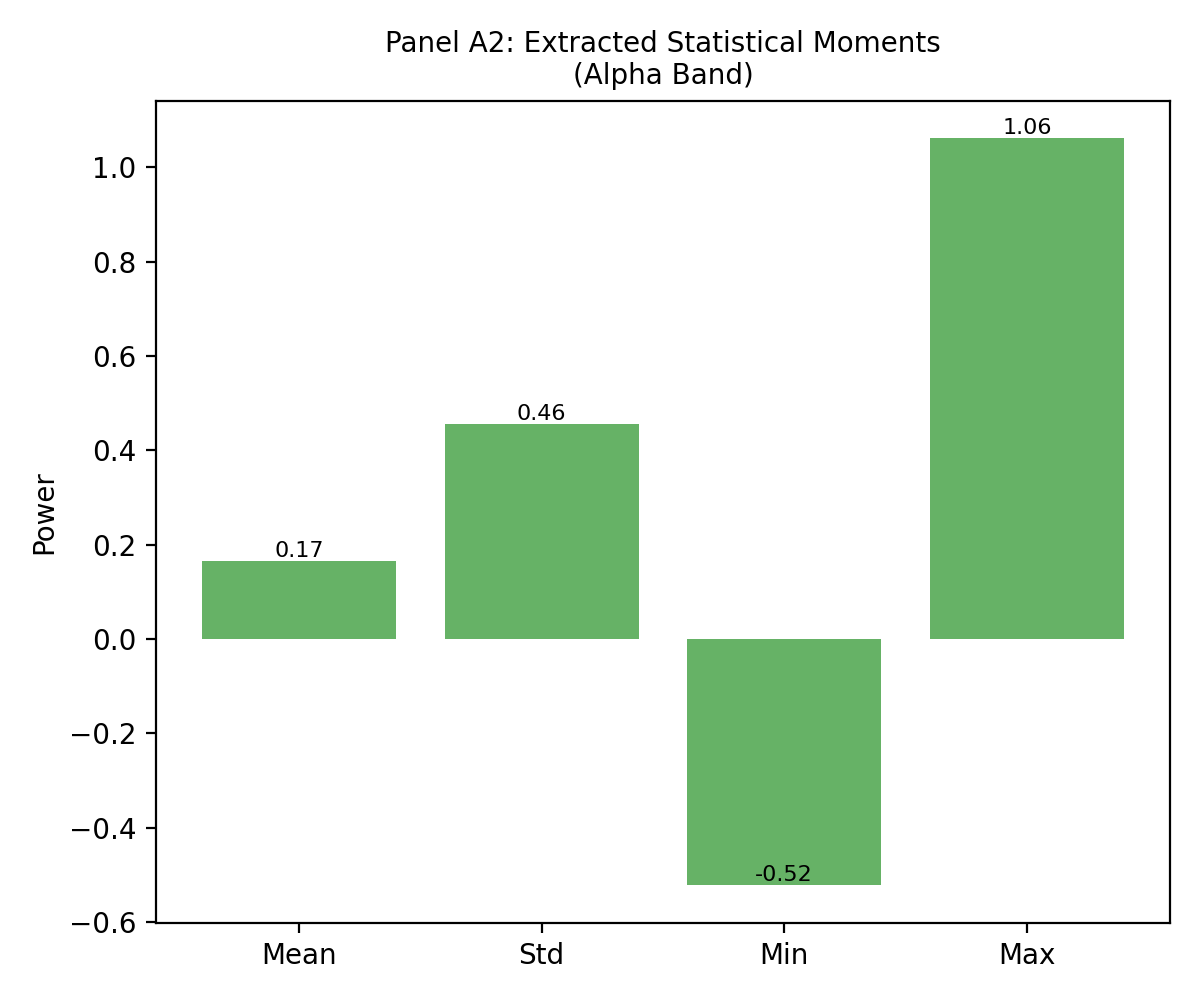
\includegraphics[width=\textwidth]{../05-12_data_analysis_and_results/runs/run_20260611_220844/viz/viz05a.A2.png}
    \caption{Extraction of standard statistical moments from the normalized EEG frequency bands.}
    \label{fig:stat_moments}
\end{figure}

\subsection{Engagement Index Calculation}
To provide a recognized clinical baseline for cognitive evaluation, the Engagement Index (EI) was calculated for each analysis window. The EI is theoretically grounded in established neurophysiological research correlating task engagement with frontal and parietal band power ratios. It is mathematically defined as:
\begin{equation}
    EI = \frac{\beta}{\alpha + \theta}
    \label{fig:formula_EI}
\end{equation}
In this pipeline, exactly one scalar Engagement Index (EI) is computed per \(1.0\)-second analysis window per participant. To calculate this single value, the signal variance (representing total band power) is first extracted for the Beta (\(\beta\)), Alpha (\(\alpha\)), and Theta (\(\theta\)) bands across each of the four individual electrodes. These four spatial variances are then averaged together to produce a single, whole-head \(\beta\), \(\alpha\), and \(\theta\) scalar for that specific window, which are finally fed into the EI ratio formula. This single composite scalar serves as the primary clinical benchmark against which the predictive power of individual statistical features is evaluated in the machine learning phase. An example calculation of the EI for a single sample window of one participant can be observed in Figure~\ref{fig:calculation_visual_EI}, visually showing the three spatially-averaged scalars that are utilized in the Index calculation in Formula~\ref{fig:formula_EI}.

% for explanation of EI definition and calculation
\begin{figure}[H]
    \centering
    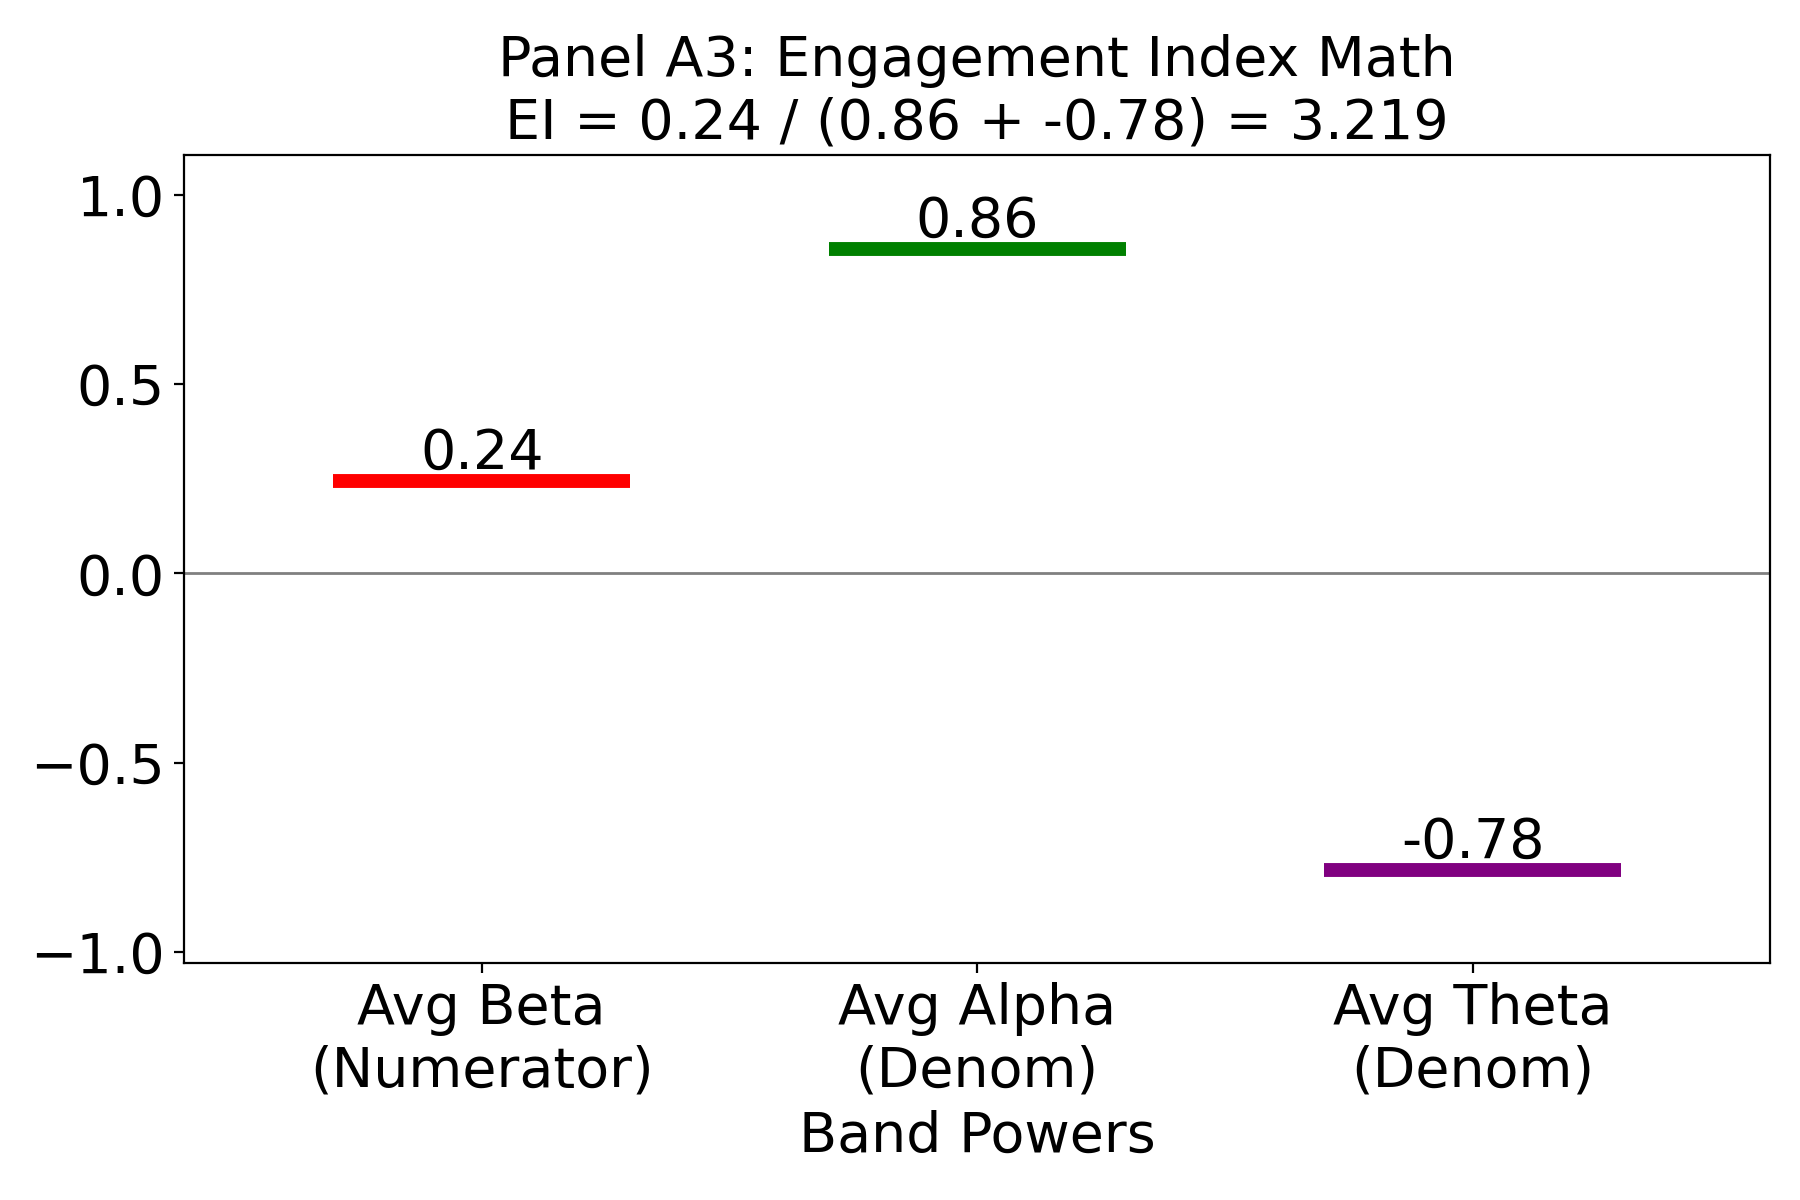
\includegraphics[width=\textwidth]{../05-12_data_analysis_and_results/runs/run_20260611_220844/viz/viz05a.A3.png}
    \caption{Engagement Index (EI) calculation deriving a single scalar engagement metric from the Beta, Alpha, and Theta band powers.}
    \label{fig:calculation_visual_EI}
\end{figure}

\subsection{Hjorth Parameters}
In addition to basic descriptive statistics, Hjorth Parameters (Activity, Mobility, and Complexity) were computed to capture the sequence-dependent temporal dynamics of the signal within the \(1.0\)-second window. While standard statistical moments characterize the amplitude distribution independently of their temporal order (i.e., they are time-invariant), Hjorth parameters depend explicitly on the time-domain derivatives, thus capturing spectral properties—such as mean frequency and bandwidth—directly from the time-domain signal.

For a discrete EEG signal vector \(y(t)\) of length \(N = 256\) representing a specific channel and frequency band within a window, the three parameters are mathematically defined as follows:

\subsubsection{Activity}
Activity measures the total signal power and is defined simply as the variance of the signal amplitude:
\begin{equation}
    \text{Activity} = \sigma_{y}^2 = \frac{1}{N} \sum_{t=1}^{N} (y(t) - \mu_y)^2
\end{equation}
where \(\mu_y\) is the mean of \(y(t)\). The input dimension is the normalized amplitude and the output dimension represents the squared amplitude.

\subsubsection{Mobility}
Mobility serves as a time-domain proxy for the mean frequency of the power spectrum. It is defined as the square root of the ratio of the variance of the first derivative \(y'(t)\) to the variance of the primary signal \(y(t)\):
\begin{equation}
    \text{Mobility} = \frac{\sigma_{y'}}{\sigma_{y}} = \sqrt{\frac{\text{var}(y'(t))}{\text{var}(y(t))}}
\end{equation}
Since the differentiation of a signal with respect to time yields a rate of change, the resulting output dimension of Mobility is expressed in Hertz (Hz).

\subsubsection{Complexity}
Complexity measures the bandwidth of the signal and indicates how closely the signal's shape resembles a pure sine wave (where a pure sine wave converges to a complexity of 1). It is defined as the ratio of the Mobility of the first derivative \(y'(t)\) to the Mobility of the primary signal \(y(t)\):
\begin{equation}
    \text{Complexity} = \frac{\text{Mobility}(y')}{\text{Mobility}(y)} = \frac{\sigma_{y''} / \sigma_{y'}}{\sigma_{y'} / \sigma_{y}}
\end{equation}
where \(\sigma_{y''}\) is the standard deviation of the second derivative of the signal. Because it is a ratio of two frequency-domain (Hz) equivalents, Complexity is a dimensionless scalar.

Together, these three parameters output exactly three scalar features per frequency band per channel, expanding the univariate feature space by explicitly encoding the temporal structural variations that basic amplitude statistics fundamentally miss.

\subsection{Peak and Macro Frequency Extraction}
Beyond traditional amplitude statistics, two specialized time-domain features were engineered to capture the dominant oscillatory and structural patterns within each specific frequency band of the \(1.0\)-second analysis window. For a discrete band-pass filtered EEG signal vector \(y(t)\) of length \(N=256\) and total duration \(T = 1.0\text{ s}\), the features are calculated as follows:

\subsubsection{Peak Frequency}
Rather than extracting the maximum bin from a Fourier transform, Peak Frequency is calculated directly in the time domain by identifying the total number of local maxima (peaks) within the signal. A point \(y(t)\) is considered a peak if it is strictly greater than its immediate neighbors. Let \(P\) be the set of all peak indices. The Peak Frequency \(f_{peak}\) is defined as the absolute peak count normalized by the window duration:
\begin{equation}
    f_{peak} = \frac{|P|}{T}
\end{equation}
The input dimension is the time-series amplitude vector, and the output is a scalar frequency representing the raw, jagged oscillatory rate of the frequency band in Hertz (Hz).

\subsubsection{Macro Frequency}
While Peak Frequency captures every local maximum, it is highly sensitive to noise and high-frequency jitter. To isolate the true, underlying macroscopic oscillatory bursts, a novel Macro Frequency algorithm was developed. 

First, a dynamic amplitude threshold \(\theta_{peak}\) is calculated as the mean amplitude of all previously identified peaks: 
\begin{equation}
    \theta_{peak} = \frac{1}{|P|} \sum_{p \in P} y(p)
\end{equation}
The signal is then converted into a binary sequence \(B(t)\) where \(B(t) = 1\) if \(y(t) \ge \theta_{peak}\) and \(0\) otherwise. 

Because a single macroscopic wave might contain slight amplitude dips that prematurely break a contiguous block of ones, the algorithm calculates the average length of all zero-sequences (gaps), denoted as \(\bar{G}\). Any gap in \(B(t)\) with a length \(g \le \bar{G}\) is mathematically bridged (converted to ones), producing a smoothed binary sequence \(B_{smooth}(t)\). 

Finally, the Macro Frequency \(f_{macro}\) is defined as the total number of distinct, contiguous blocks of ones in \(B_{smooth}(t)\), normalized by the window duration:
\begin{equation}
    f_{macro} = \frac{\text{BlockCount}(B_{smooth})}{T}
\end{equation}
The output is a stabilized, macroscopic frequency in Hertz (Hz) that robustly captures the count of dominant structural waves within the cognitive window, effectively ignoring micro-fluctuations.

\newpage
\section{Result Sythesis Pipeline}
\label{sec:method_result_synthesis_pipeline}

\subsection{Temporal Cross-Validation and Data Balancing}
Before proceeding to statistical evaluation and modeling, the inherent class imbalance depicted in Figure~\ref{fig:classes_imbalanced}, where the \texttt{STAY} class (blue) heavily dominates the \texttt{SKIP} class (red), had to be addressed (executed via \url{https://github.com/coffeeandcoffee/eeg_tiktok_pipeline/data_analysis/step04_balance_split.py}). To prevent the models from trivially predicting the majority class, the \texttt{STAY} class was randomly undersampled for each participant to achieve a strict 50/50 balance, per participant, as depicted in Figure~\ref{fig:classes_balanced}.

% this simply shows that the dominant class is STAY and for every participant different, and brings with it the demand for per participant balancing of the classes.
\begin{figure}[H]
    \centering
    \begin{minipage}{0.48\textwidth}
        \centering
        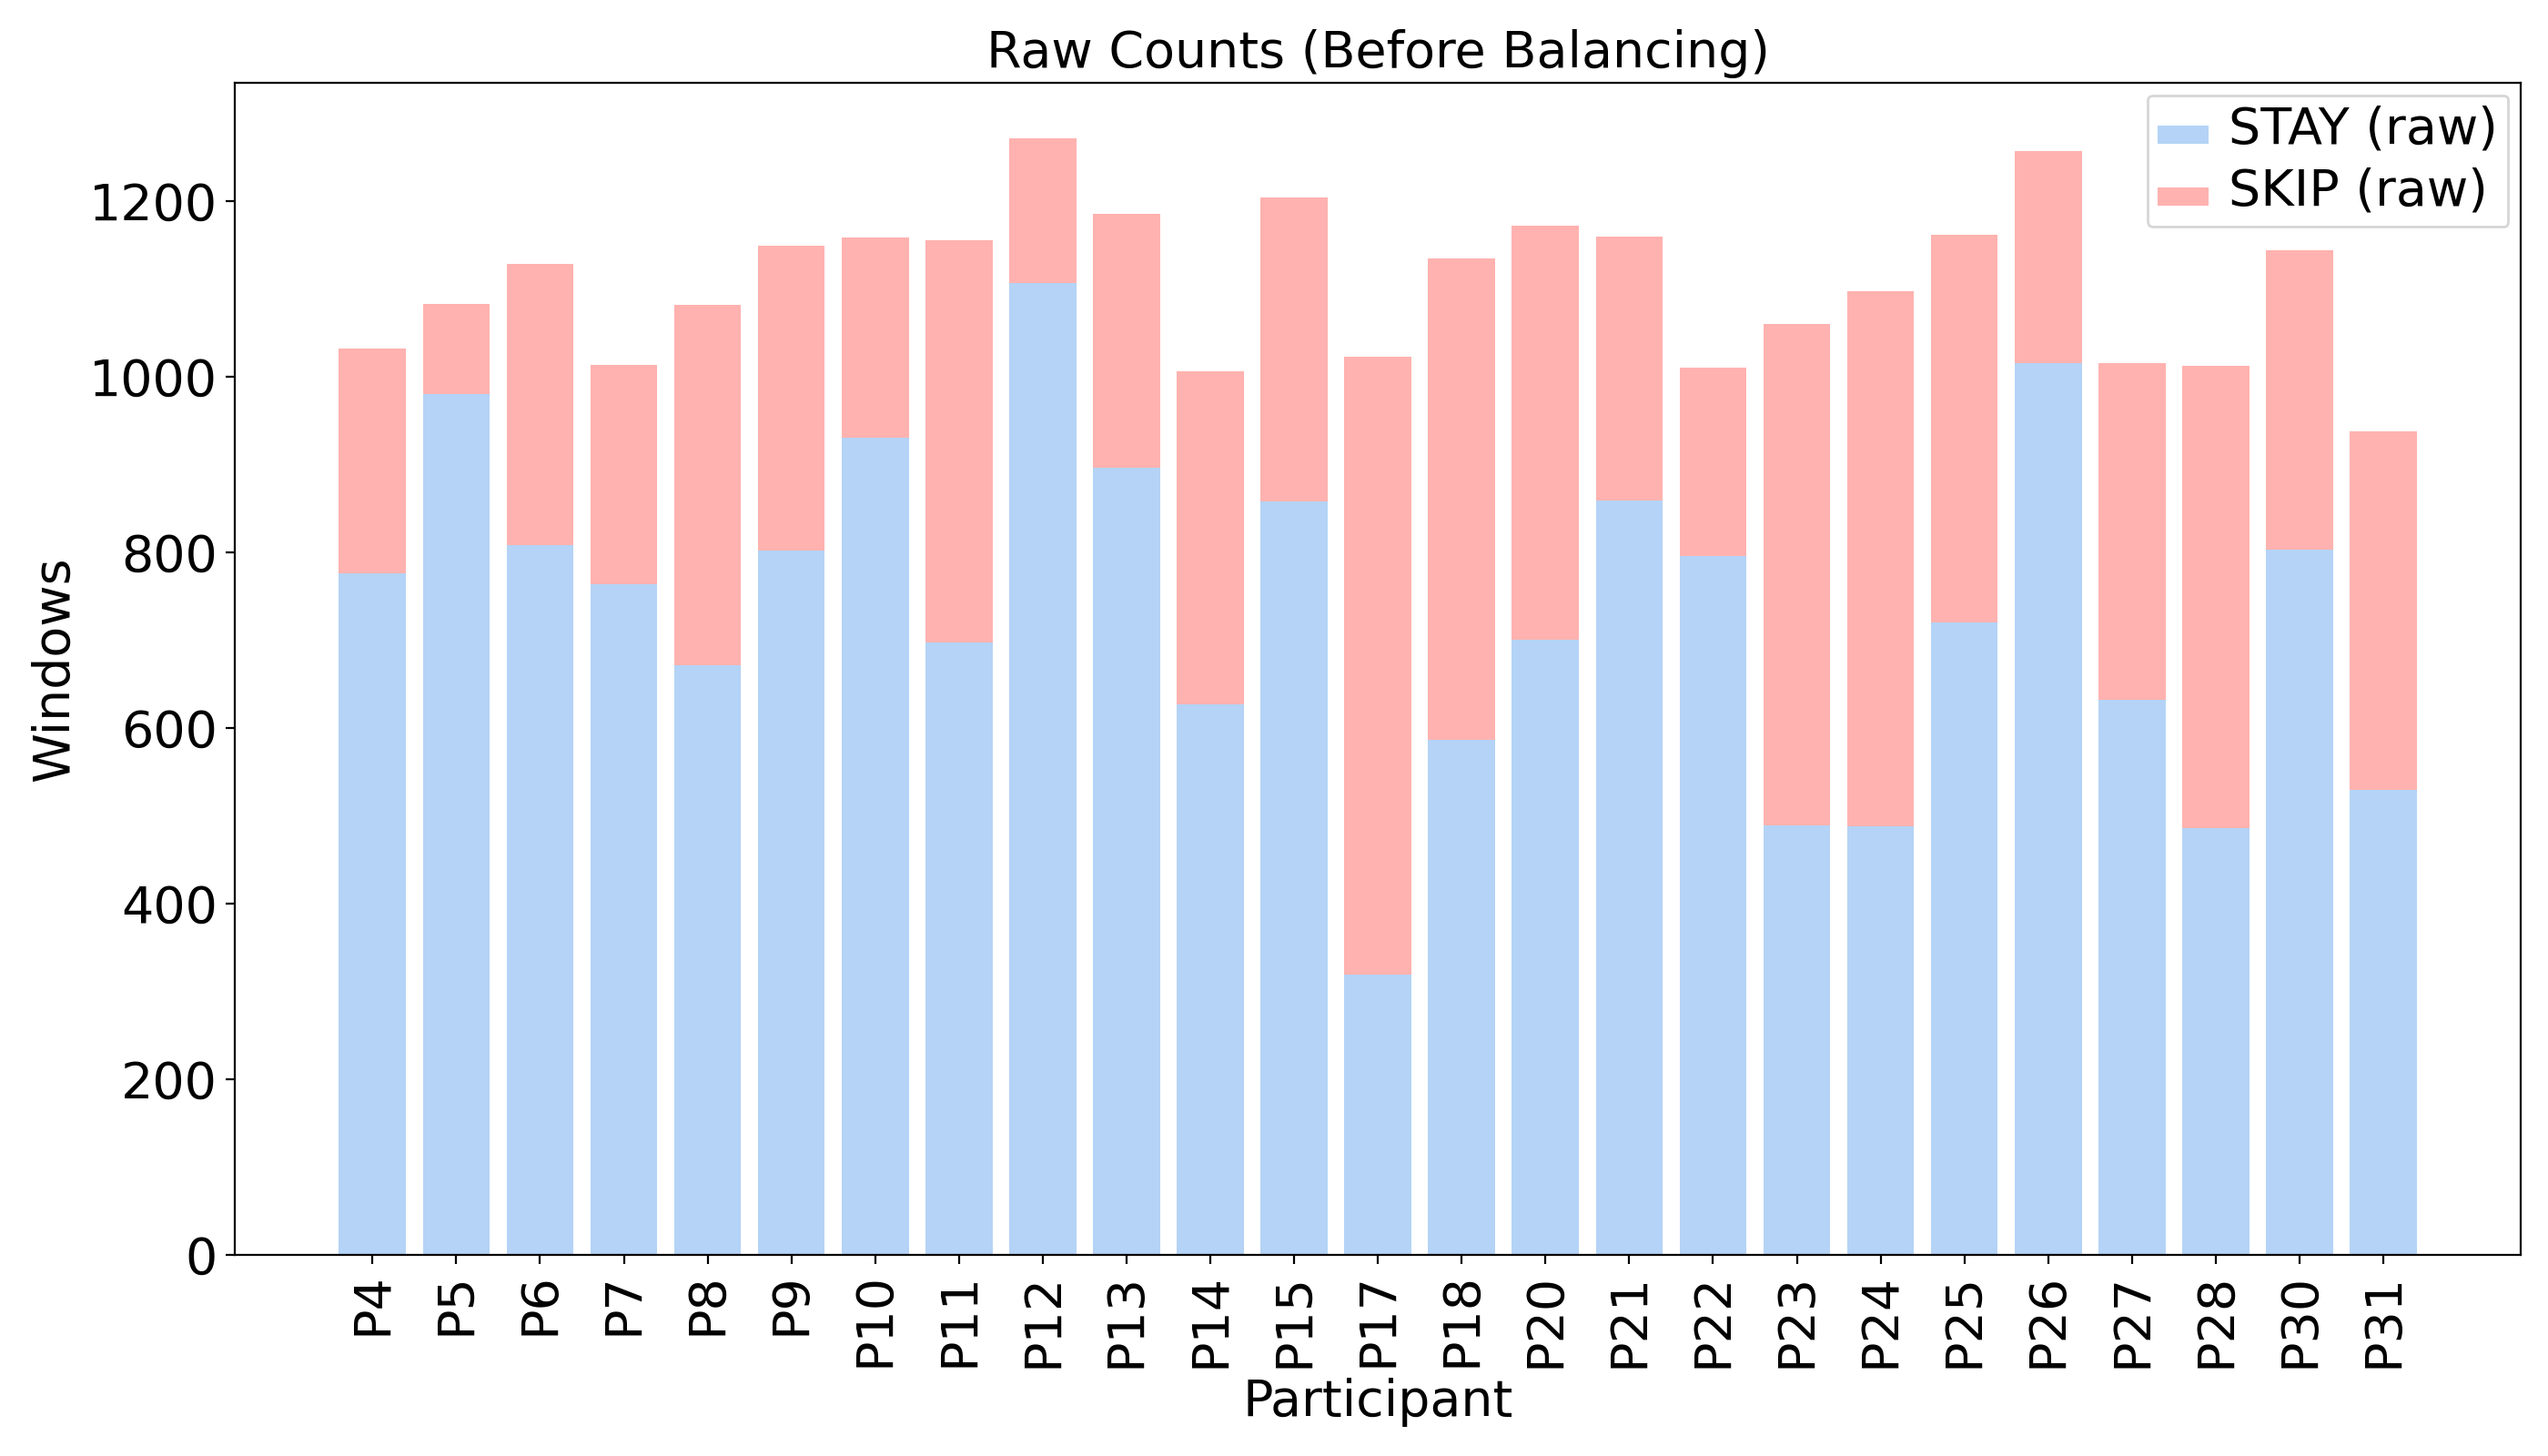
\includegraphics[width=\linewidth]{../05-12_data_analysis_and_results/runs/run_20260611_220844/viz/viz04/viz04.2_before_balancing.png}
        \caption{Raw window counts before balancing showing the extreme STAY dominance.}
        \label{fig:classes_imbalanced}
    \end{minipage}\hfill
    \begin{minipage}{0.48\textwidth}
        \centering
        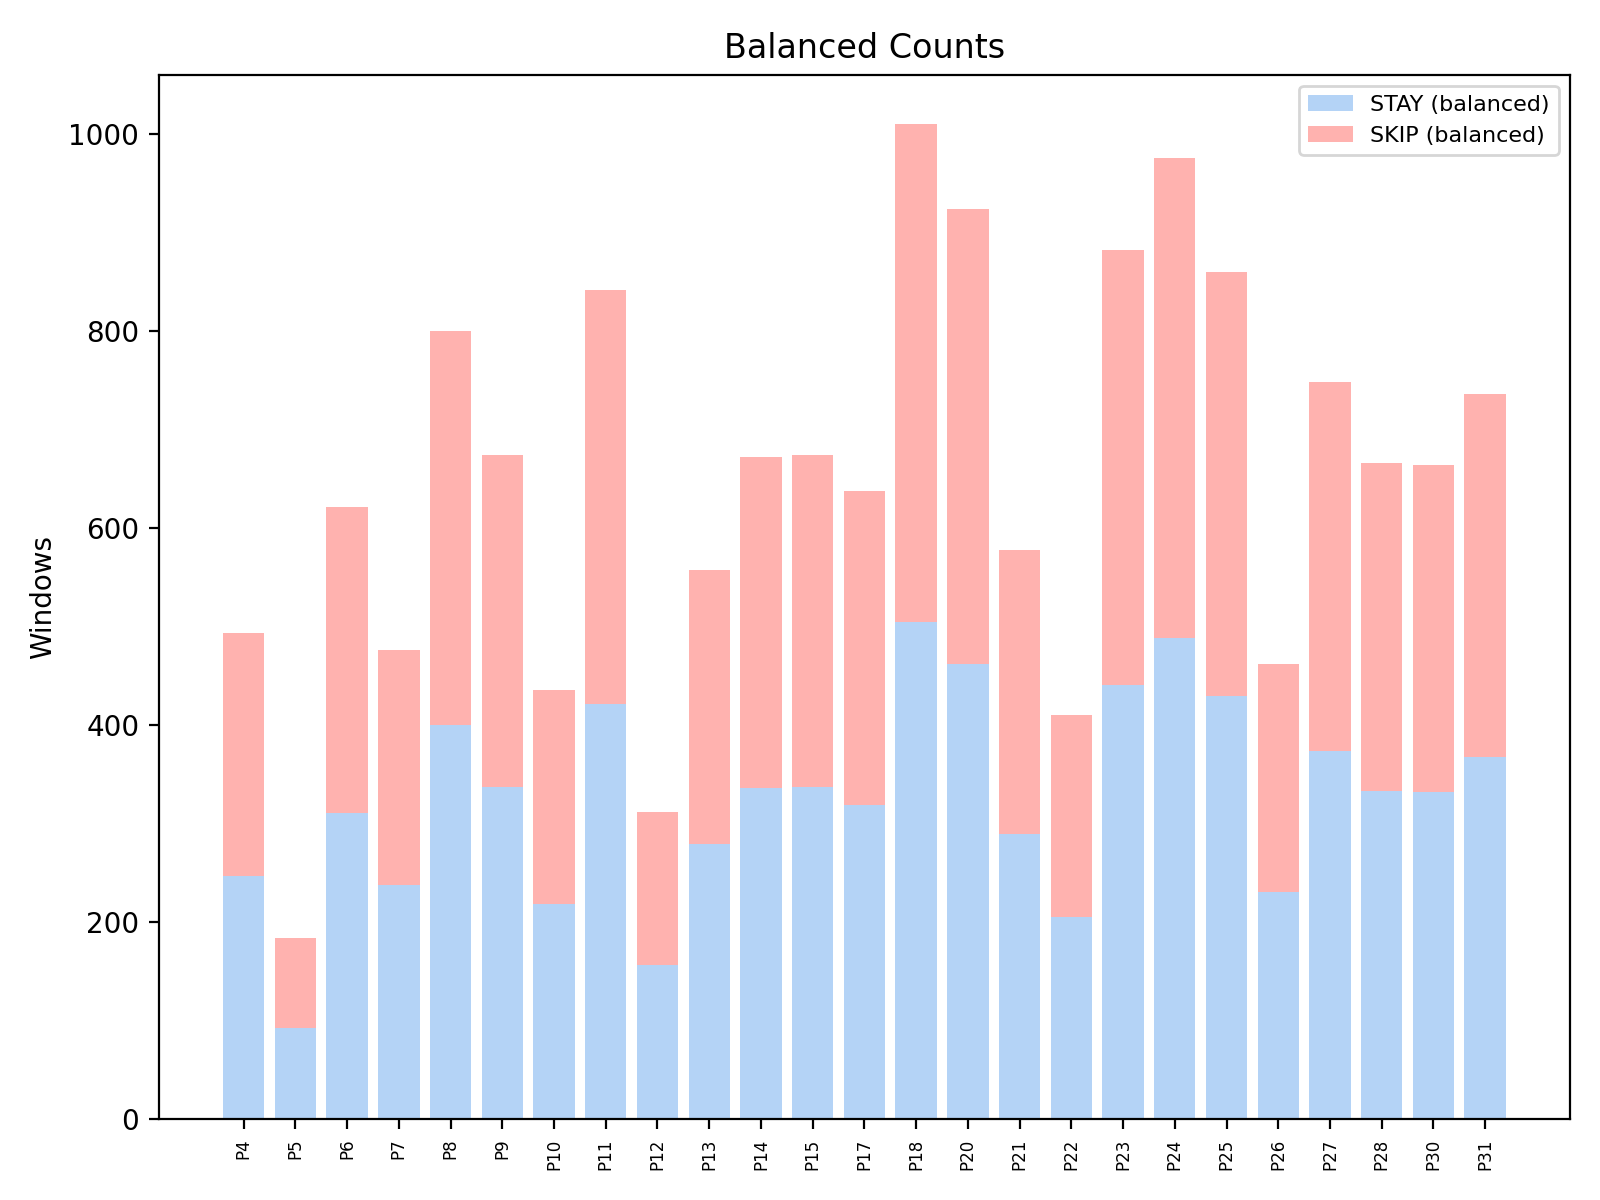
\includegraphics[width=\linewidth]{../05-12_data_analysis_and_results/runs/run_20260611_220844/viz/viz04/viz04.2_after_balancing.png}
        \caption{Window counts after undersampling, achieving a strict 50/50 ratio per participant.}
        \label{fig:classes_balanced}
    \end{minipage}
\end{figure}

To mitigate temporal leakage due to autocorrelation between adjacent EEG windows, blocked temporal 5-fold cross-validation was applied. Each participant’s data were partitioned chronologically into five folds with equal counts of minority-class (\texttt{SKIP}) instances. Figure~\ref{fig:5_fold_split_per_participant} shows minority-class occurrences (red) and fold boundaries (black), defined by equal splits of these events, per participant.

% for demonstration of how data is split into folds based on 5 equal parts of minority SKIP class per fold.
\begin{figure}[H]
    \centering
    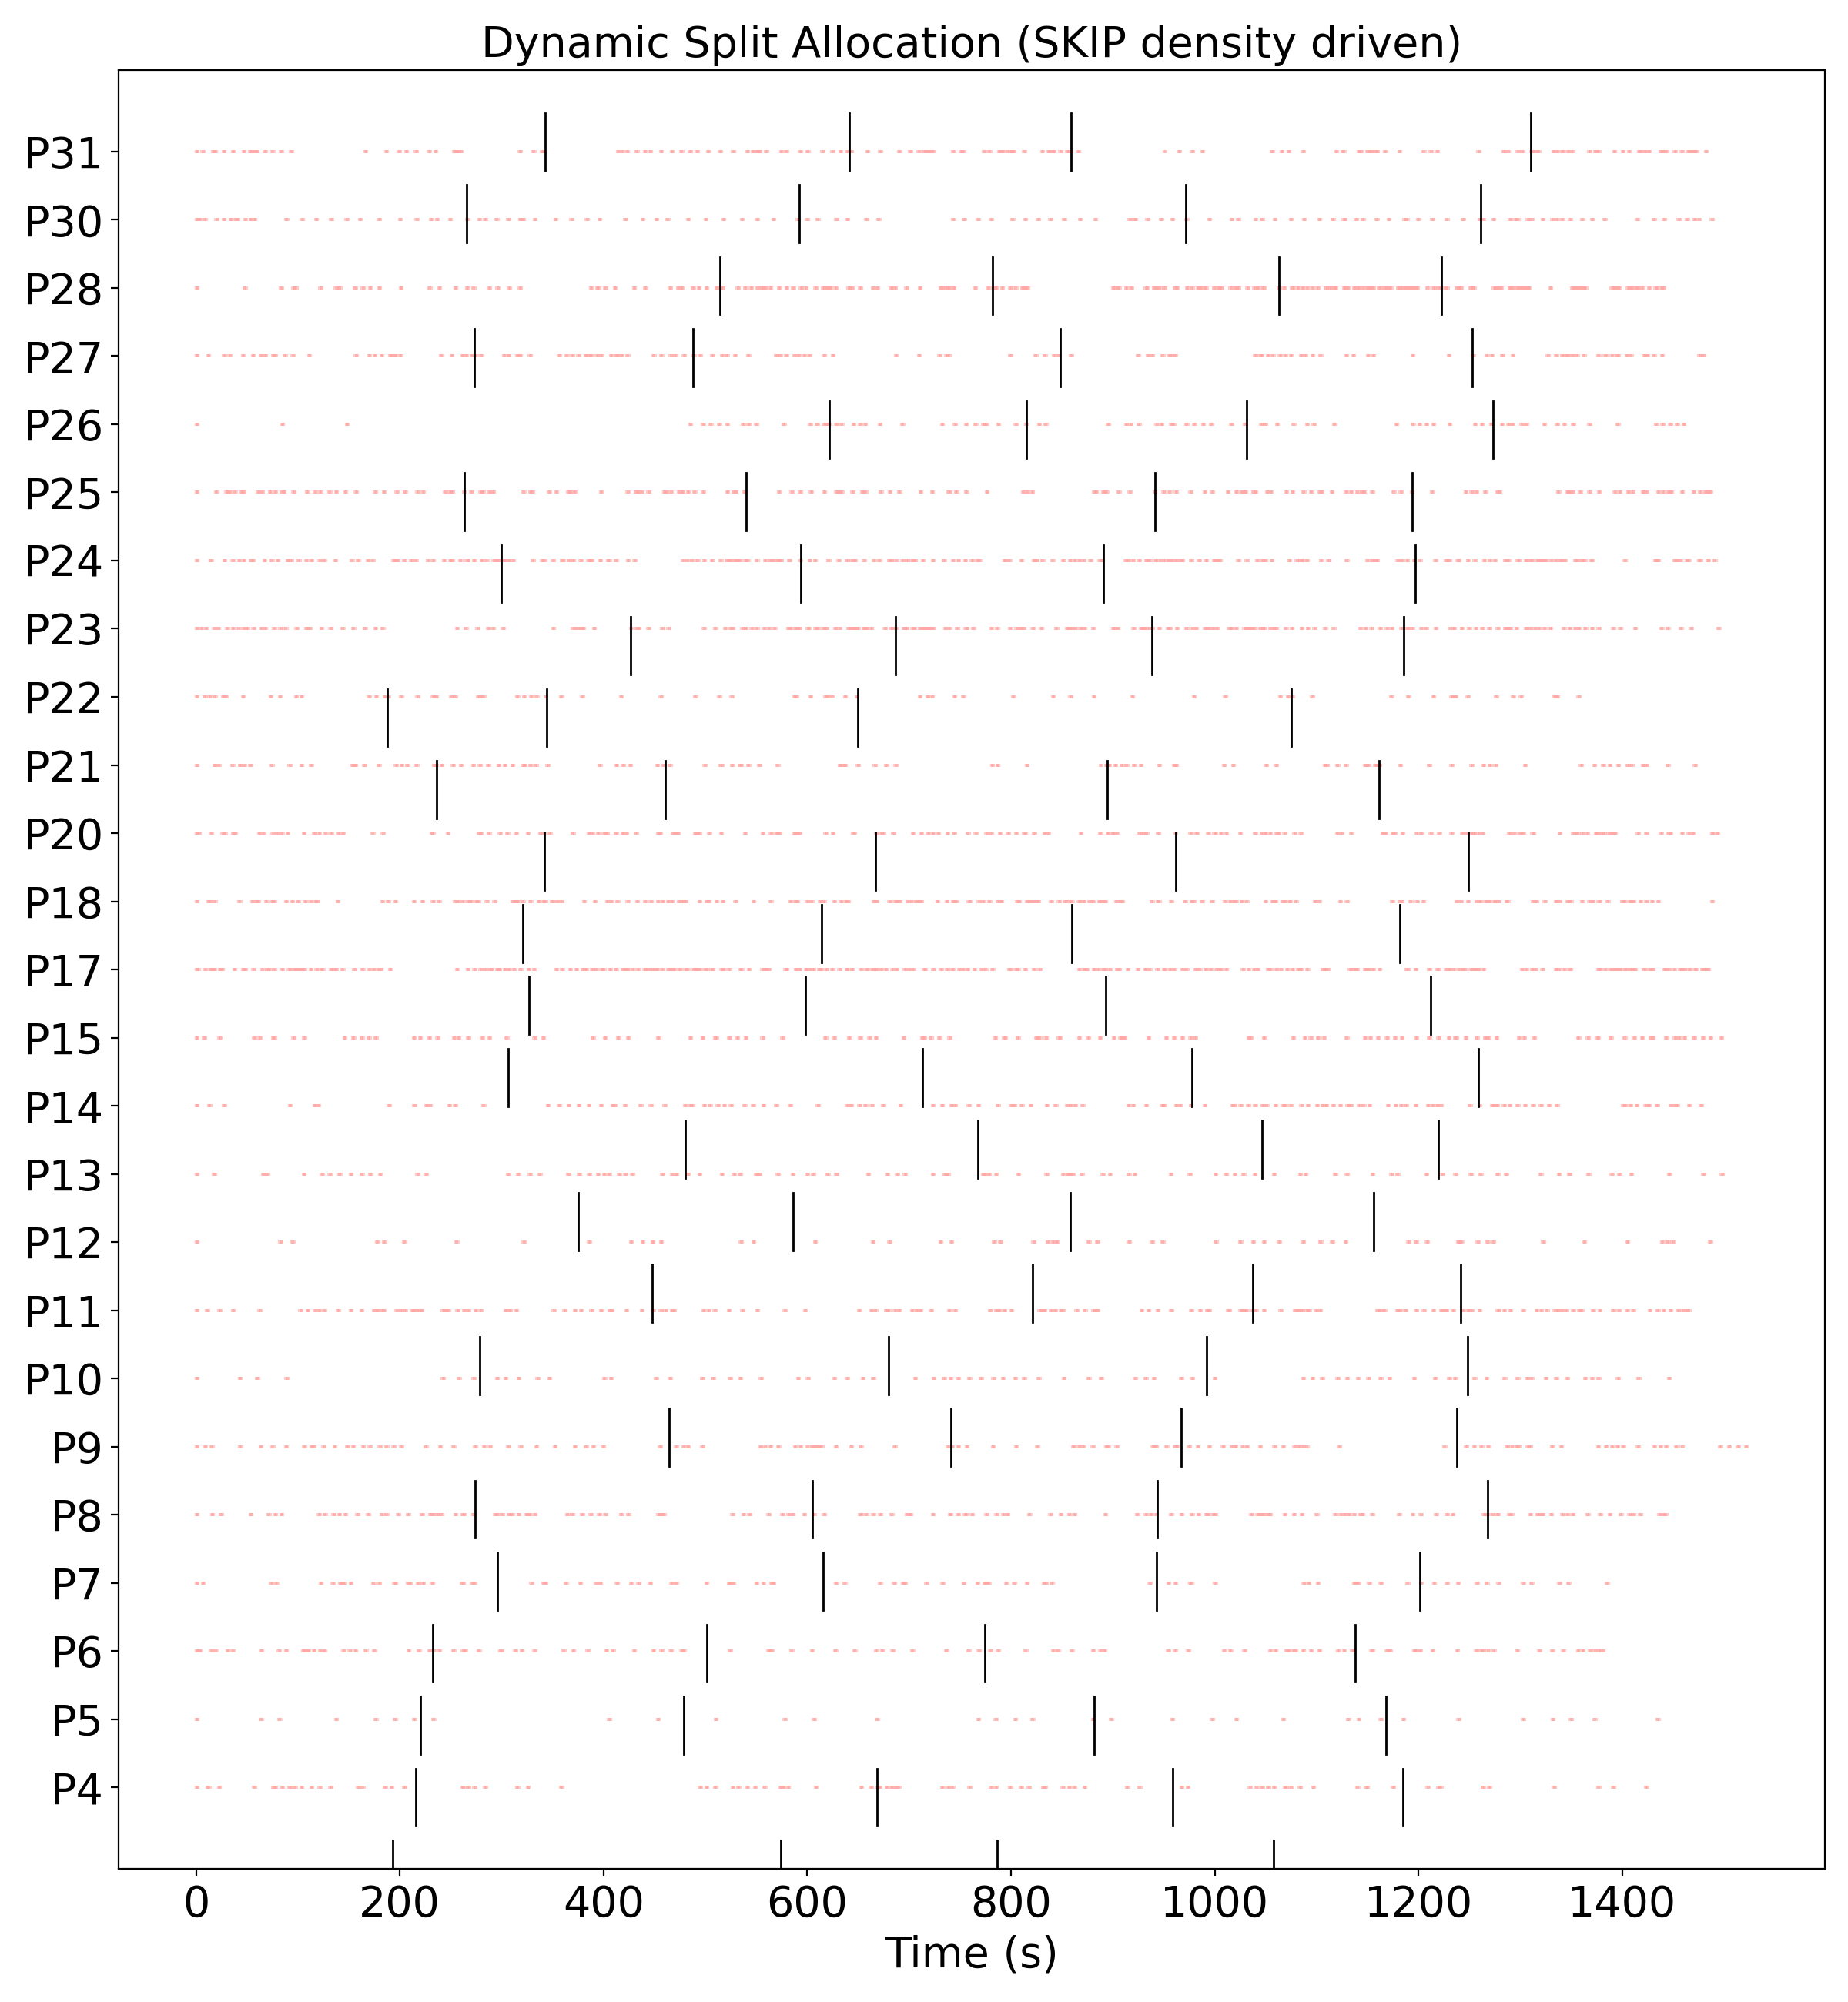
\includegraphics[width=\textwidth]{../05-12_data_analysis_and_results/runs/run_20260611_220844/viz/viz04/viz04.5.png}
    \caption{Each participant's data is temporally split into 5 folds containing equal amounts of the minority SKIP class.}
    \label{fig:5_fold_split_per_participant}
\end{figure}

To rigorously prevent temporal leakage, a minimum separation of 3 seconds between all training and testing windows was strictly enforced at every fold boundary. This constraint was implemented as a hard criterion: any violation automatically triggered pipeline termination, ensuring that no autocorrelated samples could enter the training or test sets. As verified in Figure~\ref{fig:3s_fold_boundary}, all fold boundary gaps (red points along the x-axis) exceed the predefined 3-second threshold (red dashed line), confirming compliance across the dataset. This procedure produces valid minority-balanced folds while preserving strict independence of the test data; an example for a single participant is shown in Figure~\ref{fig:fold_boundaries_for_one_participant}, where the separation gaps between folds (colored blocks) are clearly visible.

% for demonstration of the safety mechanism that ensures stricti no overlap of test and train splits, with an at least 3s minimum gap that must be obeyed as it is demonstrates to successfully be the case in this picture.
% for demonstration of how it looks with one participant, with all 5 folds in different colors.
\begin{figure}[H]
    \centering
    \begin{minipage}{0.48\textwidth}
        \centering
        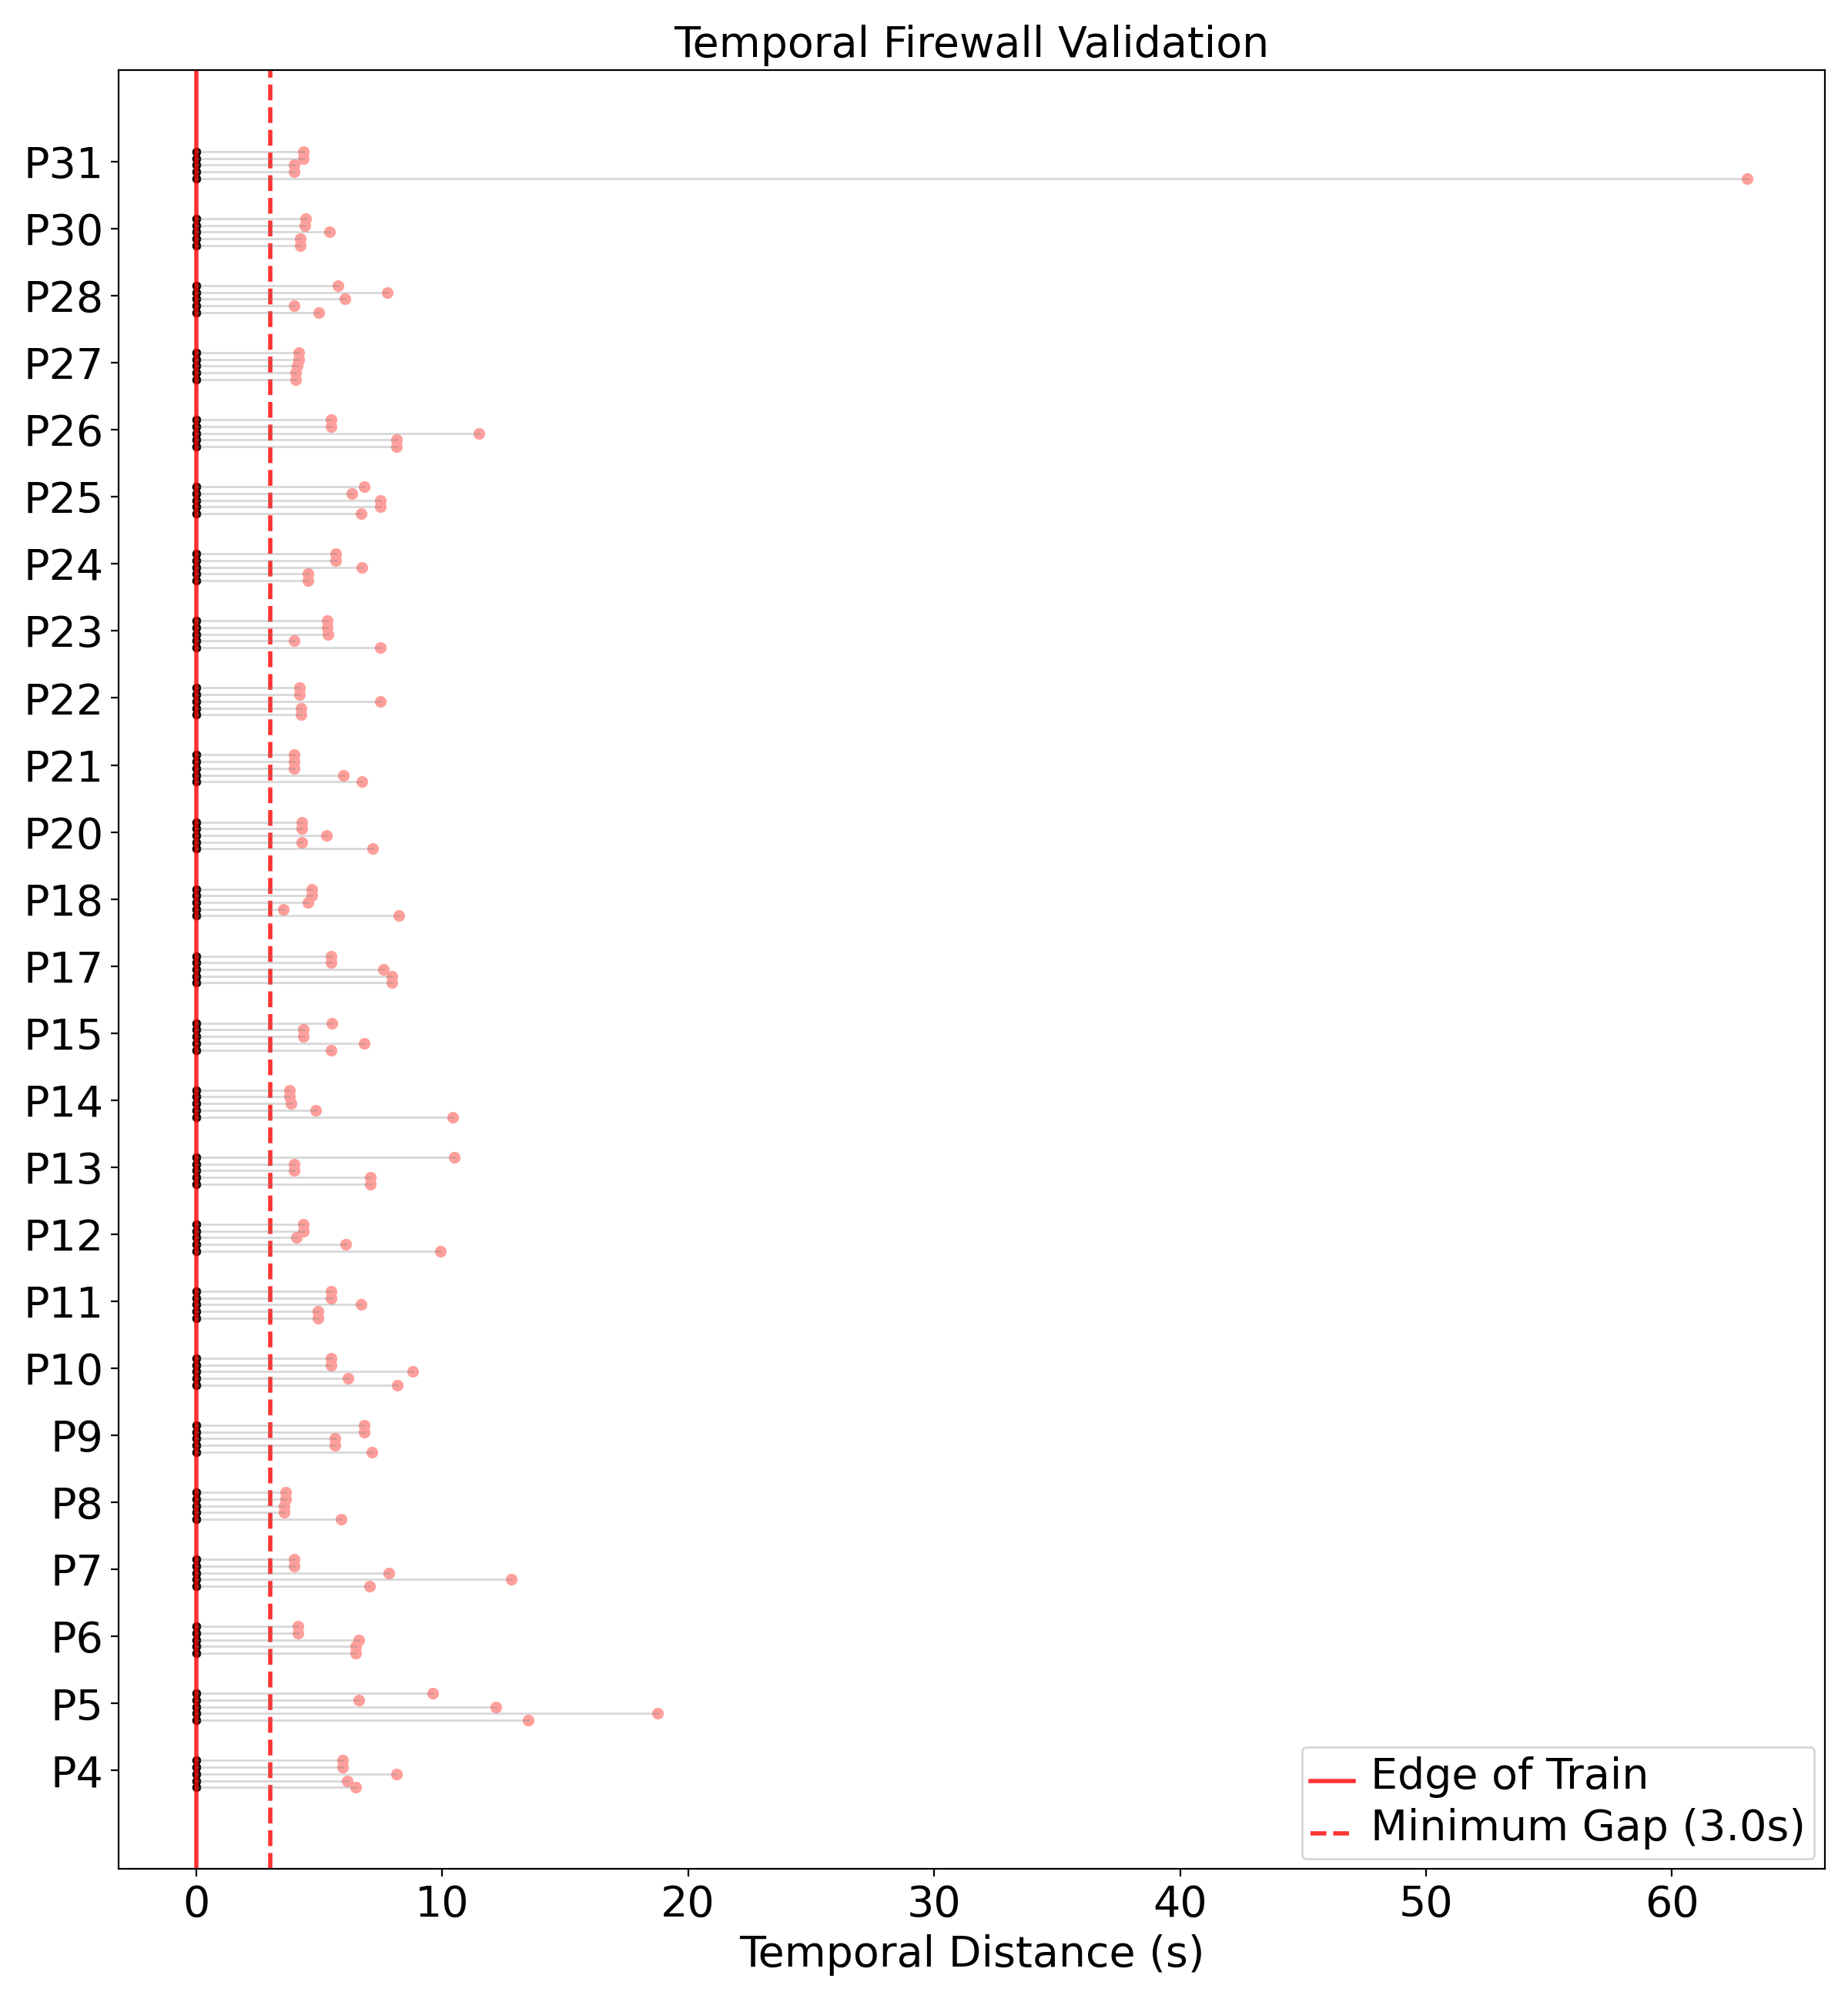
\includegraphics[width=\linewidth]{../05-12_data_analysis_and_results/runs/run_20260611_220844/viz/viz04/viz04.4.png}
        \caption{Temporal minimum required safety distance of 3 seconds between train and test windows is strictly fulfilled.}
        \label{fig:3s_fold_boundary}
    \end{minipage}\hfill
    \begin{minipage}{0.48\textwidth}
        \centering
        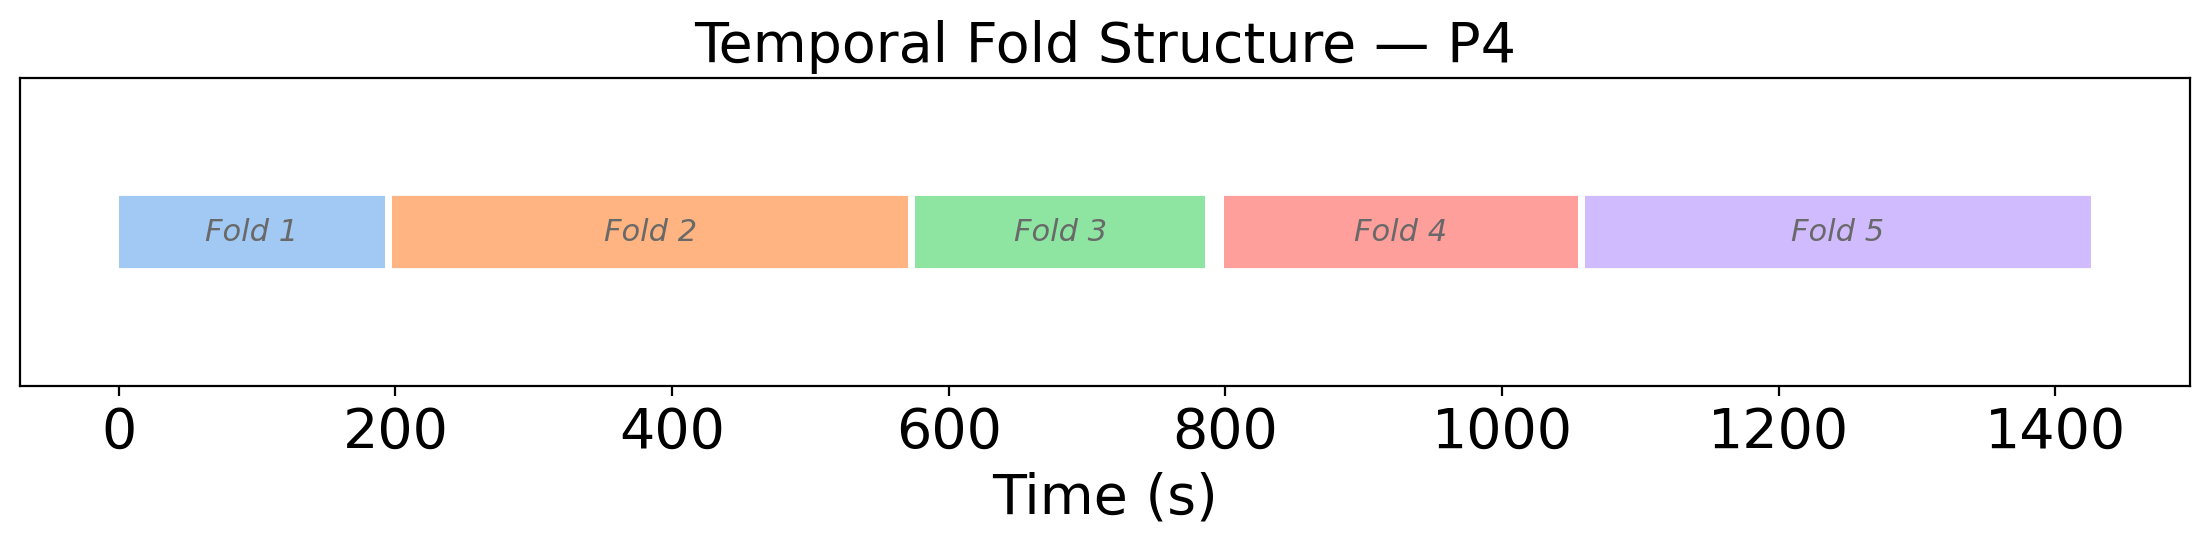
\includegraphics[width=\linewidth]{../05-12_data_analysis_and_results/runs/run_20260611_220844/viz/viz04/viz04.1.png}
        \caption{Temporal cross-validation split visualization, detailing the visible gaps between folds that successfully prevent data leakage.}
        \label{fig:fold_boundaries_for_one_participant}
    \end{minipage}
\end{figure}

\subsection{Feature Separation Analysis}
\label{sec:method_feature_separation_cohen_d}
To mathematically evaluate the discriminative power of individual features prior to modeling, Cohen’s \(d\) was computed to measure the standardized effect size between the \texttt{STAY} and \texttt{SKIP} distributions for each engineered feature (executed via \url{https://github.com/coffeeandcoffee/eeg_tiktok_pipeline/data_analysis/viz17_feature_ranking.py}). Cohen’s \(d\) is defined as
\[
d = \frac{\mu_{\text{STAY}} - \mu_{\text{SKIP}}}{s_{\text{pooled}}}
\]
where \(\mu_{\text{STAY}}\) and \(\mu_{\text{SKIP}}\) represent the class-specific sample means, and \(s_{\text{pooled}}\) denotes the pooled standard deviation. As a standardized effect size, Cohen’s \(d\) provides a scale-invariant measure of class separation that is independent of the absolute units of the feature (e.g., microvolts versus power spectral density). It quantifies how many standard deviations separate the centers of the two classes, thereby capturing theoretical separability prior to any model training.

By calculating the absolute effect size \(|d|\), the pipeline systematically ranked all extracted features (e.g., TP10\_raw\_std) according to their individual ability to separate sustained cognitive engagement from the decision to disengage. Features demonstrating the highest absolute \(|d|\) values were designated as Top Features and isolated for independent predictive baseline modeling.

\subsection{Logistic Regression Modeling and Baselines}
\label{sec:method_baselines_and_logistic_regression}
To benchmark the true predictive capability of the engineered EEG features against chance and clinical baselines, three distinct modeling approaches were evaluated on the temporally isolated test sets (executed via \url{https://github.com/coffeeandcoffee/eeg_tiktok_pipeline/data_analysis/step07_train_intra.py} and synthesized in \url{https://github.com/coffeeandcoffee/eeg_tiktok_pipeline/data_analysis/step16_parallel_universes.py}).

\vspace{1em}
\noindent\textbf{1. Coinflip Baseline:} A uniform dummy classifier (\texttt{DummyClassifier (strategy='uniform')}) was utilized to establish an empirical chance baseline. Given the rigorous 50/50 balancing of the datasets, this approach reliably generated predictions hovering around the 50\% chance level, verifying that no underlying structural bias existed within the cross-validation folds.

\vspace{1em}
\noindent\textbf{2. Engagement Index (EI) Baseline:} The pre-calculated EI scalar (derived from \(\beta/(\alpha+\theta)\)) was scaled utilizing a standard scaler (subtracting the mean and scaling to unit variance) and fed as a singular feature into a Logistic Regression model (\verb|LogisticRegression(class_weight='balanced')|). This established a clinical baseline, indicating how well classical engagement theory alone could predict the behavioral swipe decision in this specific short-form video context.

\vspace{1em}
\noindent\textbf{3. Top Feature Logistic Regression:} To test the predictive power of individual statistical features independently, the features ranked highest via Cohen's \(d\) (e.g., specific band powers or statistical moments) were similarly scaled and evaluated using isolated Logistic Regression models. This isolated approach allows for direct comparison of individual feature efficacy without the confounding complexities of high-dimensional multivariate models.

To ensure a strict one-to-one comparison with the one-dimensional Engagement Index baseline, each macro “Top Parameter” (band, electrode, statistic) was represented by its strongest single constituent feature.

\subsection{Metrics and Significance Testing}
\label{sec:method_metrics_and_significance}
To comprehensively evaluate model performance, standard classification metrics were computed for each cross-validation fold: Accuracy, Precision, Recall, and the F\(_1\)-score. In this context, correct prediction of the \texttt{STAY} class reflects successful detection of sustained cognitive engagement, whereas correct prediction of the \texttt{SKIP} class corresponds to identifying an impending disengagement decision within a 3–5 second pre-action window.

The F\(_1\)-score was used as the primary performance metric, as it balances Precision and Recall and is robust to class imbalance. Metrics were computed separately for each class by treating the respective class as the positive label (i.e., one-vs-rest evaluation for \texttt{SKIP} and \texttt{STAY}).

\textbf{Metric definitions:} Let TP, FP, TN, and FN denote true positives, false positives, true negatives, and false negatives, respectively. To achieve optimal classification performance, the correct predictions (TP and TN) must be maximized while the incorrect predictions (FP and FN) are minimized.


\[ \text{Accuracy} = \frac{TP + TN}{TP + TN + FP + FN} \]

\[ \text{Precision} = \frac{TP}{TP + FP} \]

\[ \text{Recall} = \frac{TP}{TP + FN} \]

\[ F_1 = 2 \cdot \frac{\text{Precision} \cdot \text{Recall}}{\text{Precision} + \text{Recall}} \]

\vspace{1em}
\textbf{Case 1: \texttt{SKIP} as the positive class}
\begin{itemize}
    \item \textbf{TP:} correctly predicted \texttt{SKIP} instances
    \item \textbf{TN:} correctly predicted \texttt{STAY} instances
    \item \textbf{FP:} \texttt{STAY} instances incorrectly predicted as \texttt{SKIP}
    \item \textbf{FN:} \texttt{SKIP} instances incorrectly predicted as \texttt{STAY}
\end{itemize}

\vspace{1em}
\textbf{Case 2: \texttt{STAY} as the positive class}
\begin{itemize}
    \item \textbf{TP:} correctly predicted \texttt{STAY} instances
    \item \textbf{TN:} correctly predicted \texttt{SKIP} instances
    \item \textbf{FP:} \texttt{SKIP} instances incorrectly predicted as \texttt{STAY}
    \item \textbf{FN:} \texttt{STAY} instances incorrectly predicted as \texttt{SKIP}
\end{itemize}
\vspace{1em}

A class-specific F\(_1\)-score substantially exceeding chance level indicates that the model captures discriminative structure beyond random guessing for that class. For reference, under balanced random predictions, the expected F\(_1\)-score is approximately 0.5, whereas under strong class imbalance, this baseline decreases and should be interpreted relative to the class distribution.

To rigorously evaluate whether the Logistic Regression models utilizing individual EEG features outperformed the established baselines across the participant cohort, non-parametric statistical testing was employed. Specifically, the Wilcoxon signed-rank test was used to compute the statistical significance (\(p\)-value) of the performance differences between paired model distributions (e.g., Top Feature model vs. EI Baseline model, or EI Baseline model vs. 50\% chance level) at the participant level. For each participant, the performance metric (e.g., F\(_1\)-score) of the evaluated model was contrasted with that of the baseline, yielding 25 paired differences across the Leave-One-Group-Out cross-validation folds.  

The algorithm employs a two-sided Wilcoxon test with a standard significance threshold (\(\alpha = 0.05\)). Because a two-sided test detects significant differences in either direction, a directional validation check is applied post hoc: a model is deemed statistically significantly superior only if two conditions are met simultaneously, namely (i) the test yields \(p < 0.05\), and (ii) the arithmetic mean of the model’s scores across all participants is strictly greater than the arithmetic mean of the corresponding baseline. The rank-biserial correlation (\(r\)) is also computed to quantify the effect size of the Wilcoxon test, indicating the strength of the model's superiority over the compared baseline. This structured chain of statistical proof robustly determines whether individual EEG features can provide a significant improvement over both pure chance and classical clinical engagement metrics when attempting to predict real-world short-form video interactions.



\iffalse
\section{Internal Structuring: Results Narrative and Gap Analysis}


\textit{Note: The following subsection synthesizes the data produced by the re-architected \texttt{STAY} pipeline (Case B). It provides a structured, logical story arc mapping what we set out to prove, what the data actually shows, and explicitly highlights what is missing or incomplete for the final academic narrative.}

\subsection*{INTERNAL NOTE: Scope, Claims, and Language Guardrails for Results and Conclusion Writing}
\textit{This note is for internal drafting purposes and must be removed before final submission.}

\bigskip

\textbf{The Research Question (exact formulation)}

Within a controlled proof-of-concept study, can consumer-grade EEG---using a 4-channel dry-electrode headband---reliably classify sustained cognitive engagement (\texttt{STAY}) versus imminent disengagement (\texttt{SKIP}) during naturalistic TikTok browsing at the intra-subject level? As a secondary question, and with explicit acknowledgement of the sample's demographic homogeneity, this thesis further examines whether any such intra-subject neural signature shows preliminary evidence of cross-individual consistency.

\bigskip

\textbf{What the sample actually is}

$n=25$ participants, age range 20--30, all students or affiliates of the Hasso Plattner Institute. This is a homogeneous convenience sample by definition. It is not representative of the general population, TikTok users as a demographic, or any age group outside young adults in an academic setting. This was acknowledged explicitly in the abstract and introduction. Every result sentence in this chapter must be written as if this constraint is active.

\bigskip

\textbf{The three claims you are allowed to make (UPDATED 2026-05-06 after rigorous audit)}

\begin{enumerate}
    \item \textbf{Intra-subject feasibility is established (with properly calibrated magnitude).} Using blocked temporal 5-fold CV (leakage-corrected), the RF-112 model achieves a mean accuracy of 53.8\% across 25 participants (Wilcoxon $p=0.0015$), with 20 of 25 individuals exceeding the 50\% chance baseline. The effect is small ($\sim$3.8pp above chance) but statistically significant. Three participants show strong individual performance (P12: 81.2\%, P7: 67.3\%, P22: 62.9\%). NOTE: The original 61.6\% was inflated by $\sim$8pp due to temporal data leakage from overlapping windows in a random train/test split. This leakage discovery is itself a methodological contribution.
    
    \item \textbf{Cross-subject generalization does not hold in this sample.} LOGO-CV collapses to 49.2\% accuracy. This is framed as a theoretically expected outcome given the idiosyncratic nature of higher-order prefrontal EEG, not as a methodological failure. It is also not surprising given the sample size.
    
    \item \textbf{Feature importance is broadly distributed across all frequency bands; no single band dominates.} The top 2 individual features are high\_gamma\_max at frontal sites, but at the band level, delta leads (17.5\%), followed by theta (14.8\%) and high-gamma (14.7\%). No pairwise comparison between high-gamma and other bands (except very\_high) reaches significance. The notch ablation difference is non-significant ($p=0.76$), meaning we cannot claim it ``proves'' high-gamma is genuine---only that removing the filter did not significantly degrade performance, which is \textit{consistent with} the hypothesis.
\end{enumerate}

\bigskip

\textbf{The claims you are not allowed to make}

\begin{itemize}
    \item Do not write ``these findings demonstrate that EEG can predict TikTok engagement.'' This implies generality. Write ``within this sample, these findings demonstrate...''
    \item Do not write ``users'' as a general category. Write ``participants'' or ``participants in this sample.''
    \item Do not use the word ``generalizable'' or ``representative'' anywhere in Results or Conclusion without an immediate qualifier. Your supervisor has explicitly flagged this. If you feel the urge to write either word, replace it with ``replicable in broader samples'' and add a limitation sentence.
    \item Do not frame the LOGO-CV collapse as a negative result or failure. Frame it as: the intra-subject signature is individually calibrated and does not transfer without per-user training data, which is consistent with the BCI literature and theoretically predicted by the idiosyncratic nature of higher-order cortical processing.
    \item Do not claim the 53.8\% result is clinically meaningful or practically deployable. It is a proof-of-concept accuracy in a controlled lab setting with a balanced 50/50 class prior that does not reflect real-world base rates.
    \item Do not claim the original 61.6\% accuracy. That number was inflated by data leakage. The corrected number (53.8\%, blocked temporal 5-fold CV, $p=0.0015$) is the only defensible result.
    \item Do not claim high-gamma ``dominates'' or is ``universally the dominant predictive signature.'' It ranks \#3 of 7 bands by aggregate Gini importance.
    \item Do not claim the notch ablation ``proves'' high-gamma is genuine signal. The difference is non-significant ($p=0.76$).
\end{itemize}

\bigskip

\textbf{The correct epistemic register for every result sentence}

Every quantitative result should be written in this structure:\\
\textit{``Within this sample, [finding], suggesting [limited mechanistic claim], though replication in demographically diverse samples is required before broader conclusions can be drawn.''}

You do not need to write this full sentence every time. But every result paragraph should contain at least one instance of this register before moving to interpretation.

\bigskip

\textbf{Why the proof-of-concept framing is the strongest possible position}

A reviewer or committee member cannot attack a proof-of-concept claim for lacking a large representative sample --- that is not what a proof of concept promises. The attack is pre-empted by the framing. The danger is only if you drift into generality language mid-results and contradict the scoping you established in the abstract and introduction. Consistency of register across abstract, introduction, results, and conclusion is the entire defense.
\fi

% -- results read until here -- continute reading, continute inserting INSERT: ...
% next step: continute detailled reading FEINSCHLIFF + in perplexity rephrasing.

\chapter{Results and Discussion}

This chapter presents the results of a multi-stage experimental investigation. This thesis delivers five core scientific contributions:

\begin{enumerate}
\item \textbf{Primary EEG Experiment under Naturalistic Conditions}

The foundation of this work is the primary experiment (Methods Section~\ref{sec:method_participants} - \ref{sec:method_experimental_protocol}, Results Section~\ref{sec:results_exp_learnings}), in which participants were recorded via EEG while engaging in naturalistic TikTok browsing. This data collection phase constituted a substantial portion of the overall effort, requiring careful experimental design, technical implementation, and data acquisition under ecologically valid conditions. Not only the resulting dataset, but also the easily reproducable nature of the developed experimental method forms the basis for all subsequent analyses and should be understood as a central contribution of this thesis.

\item \textbf{Reusable EEG Processing and Analysis Pipeline}

In addition to the experimental dataset and process, a further key contribution lies in the development of a comprehensive script library and analysis pipeline (Methods Section \ref{sec:method_skipstay_labeling_strategy} - \ref{sec:method_result_synthesis_pipeline}, Results Section~\ref{sec:results_pipeline}). This framework enables fully reproducible processing, from automated EEG recording on standard laptop hardware to feature extraction, class separation, and machine learning-based prediction. As such, it not only supports the present analysis but also provides a transferable methodological toolset that can be readily adapted to related experimental paradigms.

\item \textbf{Behavioral Swipe-Burst Phenomenon}

We continue by focusing on the behavioral burst analysis (Methods Section~\ref{sec:method_behavioral_burst_analysis}, Results Section~\ref{sec:results_burst_analysis}). As no burst rejection was implemented—due to scope constraints outlined in Section~\ref{sec:method_behavioral_burst_analysis}, this component is treated as a secondary result rather than the central analytical pathway.

\item \textbf{Evaluating the Engagement Index's Predictive Capacity}

The primary results emerge from a multi-layer analysis (Methods Section~\ref{sec:method_feature_engineering} - \ref{sec:method_result_synthesis_pipeline}, Results Section~\ref{sec:results_engagement_index}): Using the Cohen’s d method described in Section~\ref{sec:method_feature_separation_cohen_d}, first class separation capability of the conventional Engagement Index was evaluated, then specific features were identified that most effectively differentiate between the SKIP and STAY classes (Section~\ref{sec:results_feature_importance}) and which features outperform the Engagement Index's class-separation capability of \texttt{SKIP} and \texttt{STAY}. Building on this, a set of machine learning models as described in Section~\ref{sec:method_baselines_and_logistic_regression} is applied to predict scrolling behavior based on these class distinctions using the Engagement Index with a Logistic Regression and comparing it to a random-chance baseline, as well as challenging the conventional Engagement-Index by using previously identified superior features with the same Logistic Regression approach and comparing it to the Engagement Index. Best-performing models and features are reported (Section~\ref{sec:results_model_performance}).

As described in Section~\ref{sec:method_metrics_and_significance}, these results are carefully introduced along their statistical significance, a crucial measure considering the sample size of n=25 participants, in order to give result metrics such as the F1-score the appropriate context for meaningful interpretation for discussion and further use. While this prediction task serves as an initial proof of concept, it already indicates which features may provide sufficient discriminatory power.

\item \textbf{Neuroscientific and Behavioral Interpretation}

The results (Section~\ref{sec:results_feature_importance}) offer insights into the brain regions and frequency bands most predictive of this behavior, thereby informing both theoretical interpretation and potential practical applications. Therefore, in the final section (Section~\ref{sec:results_interpretation}), these findings are interpreted in the context of neuroscience, psychology, and behavioral research, highlighting their implications and real-world relevance.
\end{enumerate}

% ----- SECTIONS RESULTS -----

\section{Key Findings from the Experimental Paradigm}
\label{sec:results_exp_learnings}

The experimental paradigm proved feasible in a semi-controlled but still naturalistic setting, and several practical lessons emerged from its execution. Recruitment via email outreach and student mailing lists worked well, especially when paired with a clear and modest incentive. Participants were generally receptive to the study, and most were academically oriented, which appeared to increase interest in the research question and reduce concerns about signing the consent and data-protection forms.

A particularly useful element was the use of iOS Guided Access during both the baseline and TikTok phases. It provided a simple way to constrain the task environment, prevent app switching, and automatically track the duration spent in each app, which matched the temporal structure of the design well. This was especially helpful for the 2-minute baseline and the 25-minute scrolling phase, where reliable timing was essential.

At the same time, the study also highlighted several practical challenges. One recurring difficulty was maintaining a strict and consistent script during participant instruction, especially when explaining what participants should do when the task started, paused, or ended. Another challenge was ensuring that the instructions around synchronization, keypress behavior, and task boundaries were communicated clearly and uniformly across sessions. These issues did not invalidate the experiment, but they do suggest that the protocol would benefit from a more standardized briefing script and a more formalized session flow in future replications.

\section{The Reusable Methodological Pipeline}
\label{sec:results_pipeline}

A major practical contribution of this thesis is the reusable analysis and recording pipeline, which can be accessed through the associated GitHub repository, first mentioned in \ref{sec:method_data_acquisition} and further described in Section \ref{sec:method_universal_recording_pipeline}. In the present study, the pipeline ran mostly smoothly after multiple months of optimization, and finally enabled the full workflow from recording to preprocessing, feature extraction, and analysis. The main technical interruptions were occasional Bluetooth dropouts, which were handled by the recording architecture without causing major session failures, but which still underline the need for continued robustness improvements.

The development process also revealed an important software-engineering lesson: a substantial portion of the code base became obsolete during the iterative refinement across multiple months. Precisely 69.6\% (representing a reduction from 37,189 to 11,311 total lines of code) of the scripts were temporary, diagnostic, or superseded by improved versions during development. While this is normal in an exploratory research pipeline, it also shows that the project would benefit from a more systematic cleanup strategy in future iterations. A lightweight script-archiving or pruning mechanism should therefore be introduced next time to preserve clarity, reduce maintenance burden, and make the final codebase easier to reuse and extend.

More broadly, the pipeline demonstrates that a relatively compact and open methodological framework can support consumer-grade EEG recording, synchronized behavioral logging, preprocessing, and downstream feature analysis in a reproducible way. That makes it not only useful for this thesis, but also transferable to other studies with similar naturalistic EEG and behavior-synchronization requirements.

\section{Behavioral Swipe-Burst Phenomenon} \label{sec:results_burst_analysis}

As established in the methodology (Section~\ref{sec:method_behavioral_burst_analysis}), a burst is defined as a sequence of rapidly successive skip events reflecting frantic swiping. To quantify this burst severity, overlapping \texttt{SKIP} windows were grouped into “burst blocks.” The block size $n$ denotes the number of consecutive rapid swipes before a participant pauses to engage. A block of $n=1$ represents standard behavior, whereas larger values (e.g., $n=3$) indicate repeated rapid skipping, possibly without meaningful engagement due to high frequency and action state innertia.

Figure~\ref{fig:bursts_indiv_3s} shows this behavior at the participant level, revealing a clear dichotomy: some participants exhibit frequent large burst blocks (“fast scrollers”, eg P17), while others predominantly show $n=1$ behavior (“careful scrollers”, eg. P15). Figure~\ref{fig:bursts_all_3s} aggregates these patterns, confirming that while $n=1$ dominates, a long tail of burst behavior persists.

Finally, Figure~\ref{fig:bursts_all_5s} illustrates the sensitivity to the chosen window size by repeating the analysis with a ±5.0-second window (10.0-second merge threshold). The wider threshold captures a larger portion of the dwell time distribution and merges many isolated swipes into larger burst blocks, substantially reducing the proportion of $n=1$ events, simply by changing the definition of a "burst block". Specifically, under the \(\pm3.0\)s window paradigm, 67.4\% of all swipe events are isolated \(n=1\) sequences (participant-level average: 69.1\% \(\pm\) 16.2\%). In contrast, widening the window to \(\pm5.0\)s reduces the overall proportion of isolated swipes to 48.9\% (participant-level average: 46.9\% \(\pm\) 20.8\%).
 This underscores the strong dependence on parameter selection and the need for systematic optimization in future work.

\begin{figure}[H]
    \centering
    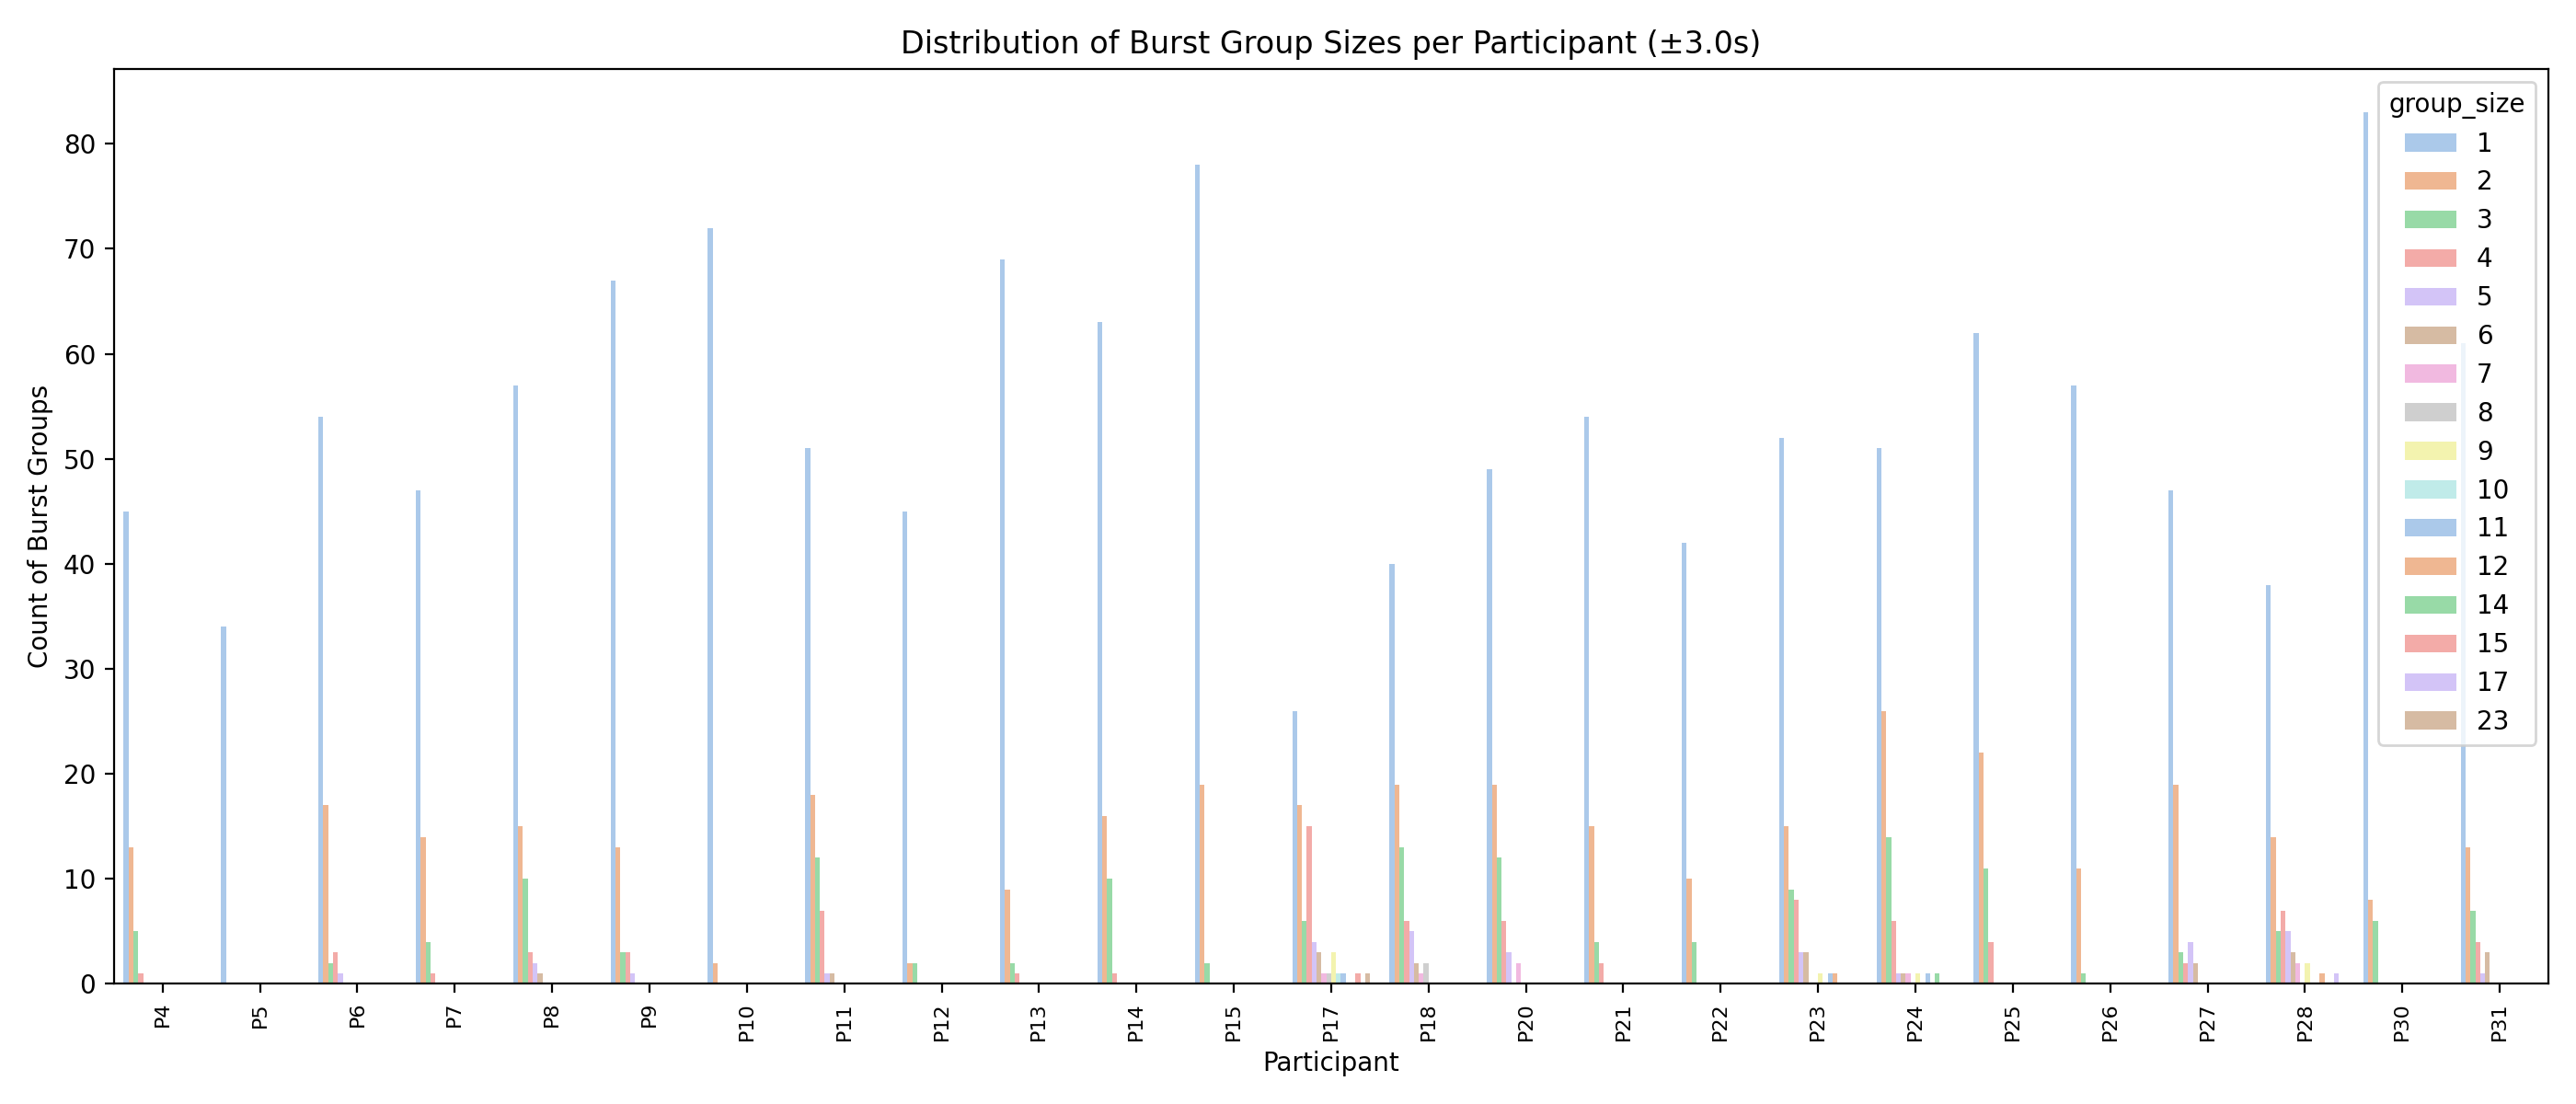
\includegraphics[width=\textwidth]{../05-12_data_analysis_and_results/runs/run_20260611_220844/viz/viz03/viz03.3.2_3s.png}
    \caption{Distribution of burst group sizes per participant (using the \(\pm3.0\)s window). This highlights the distinct behavioral difference between "frantic scrollers" (larger burst blocks) and "careful scrollers" (predominantly isolated \(n=1\) swipes).}
    \label{fig:bursts_indiv_3s}
\end{figure}

\begin{figure}[H]
    \centering
    \begin{minipage}{0.49\textwidth}
        \centering
        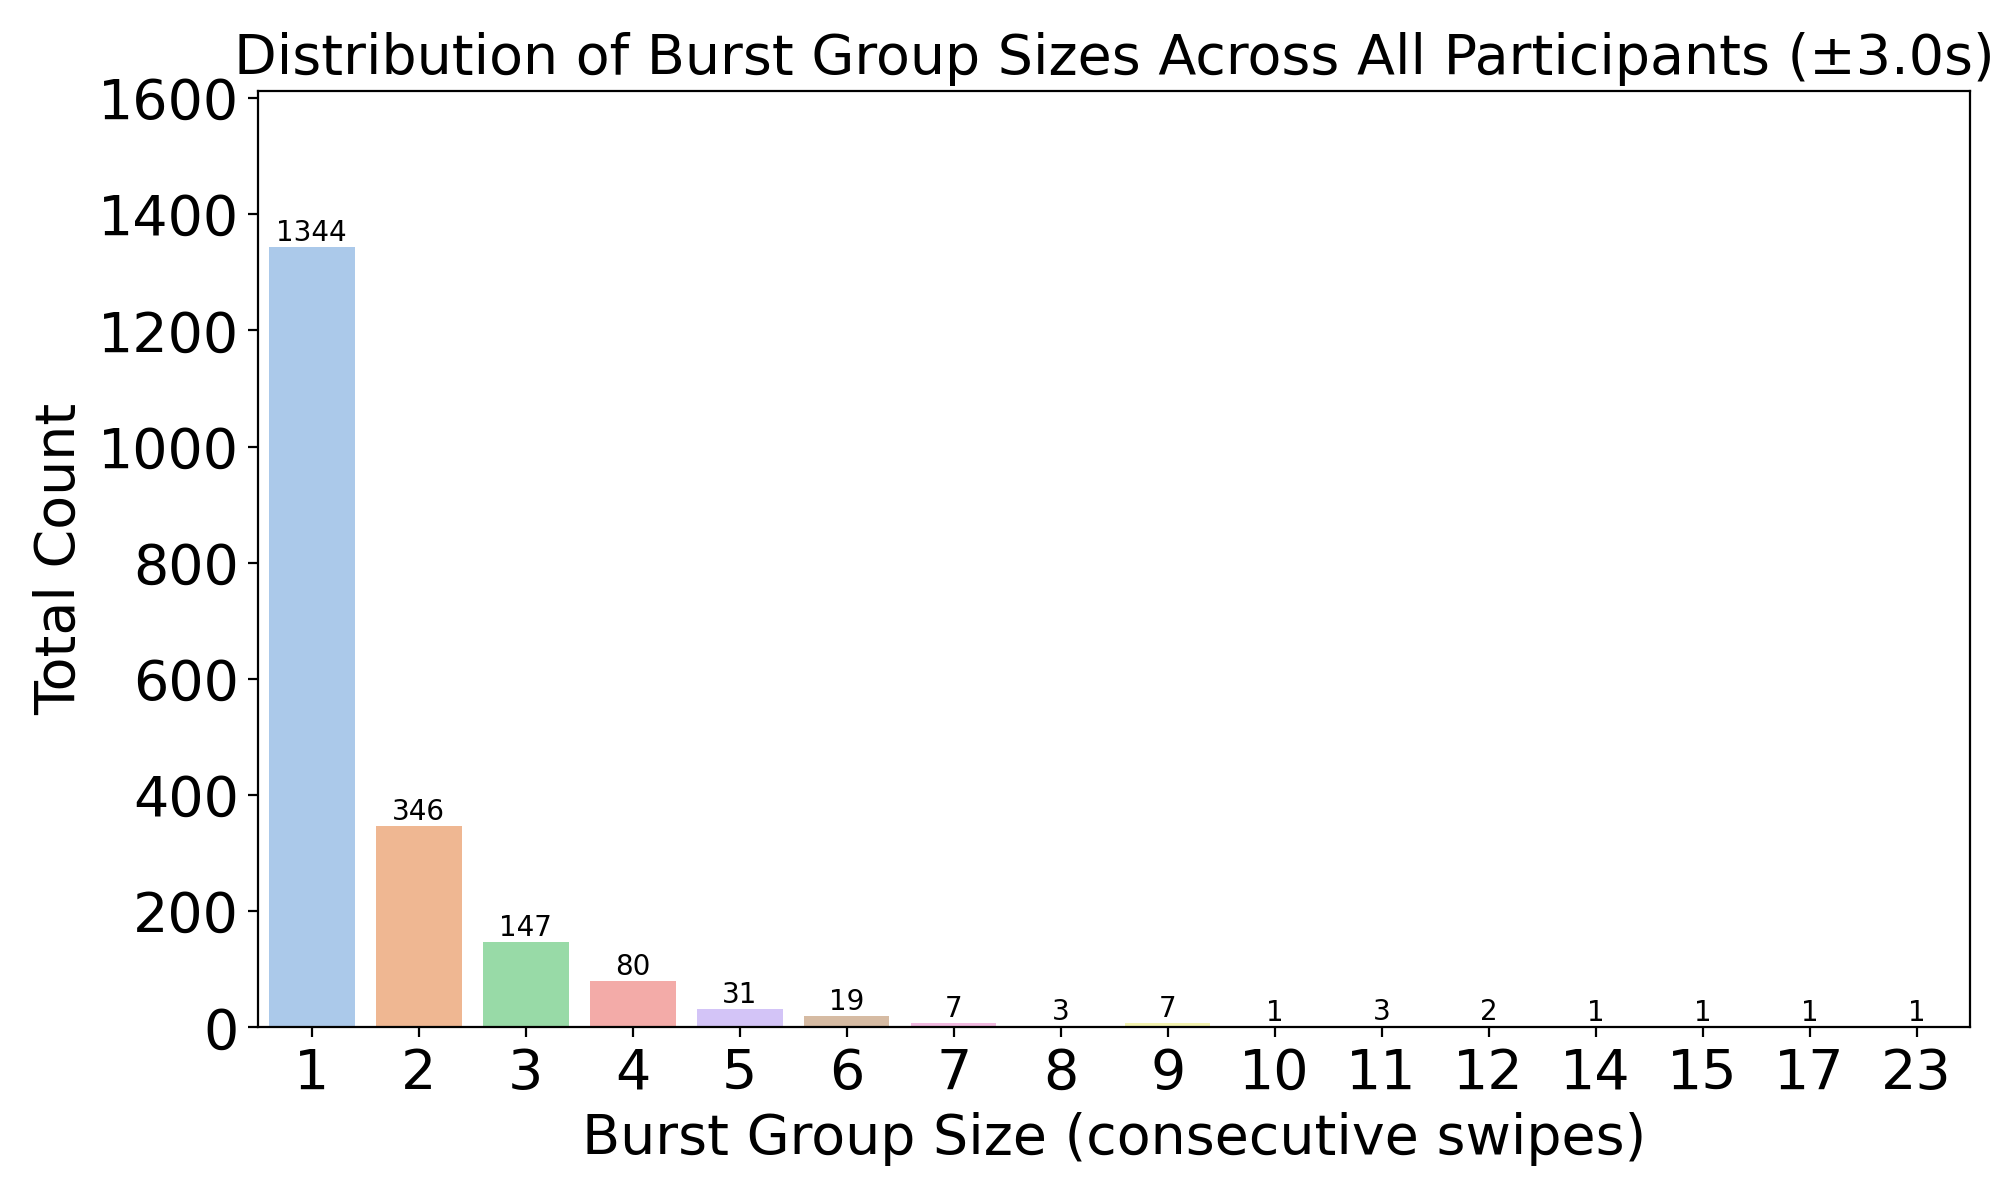
\includegraphics[width=\textwidth]{../05-12_data_analysis_and_results/runs/run_20260611_220844/viz/viz03/viz03.3.3_3s.png}
        \caption{Total burst group sizes across all participants (\(\pm3.0\)s window).}
        \label{fig:bursts_all_3s}
    \end{minipage}\hfill
    \begin{minipage}{0.49\textwidth}
        \centering
        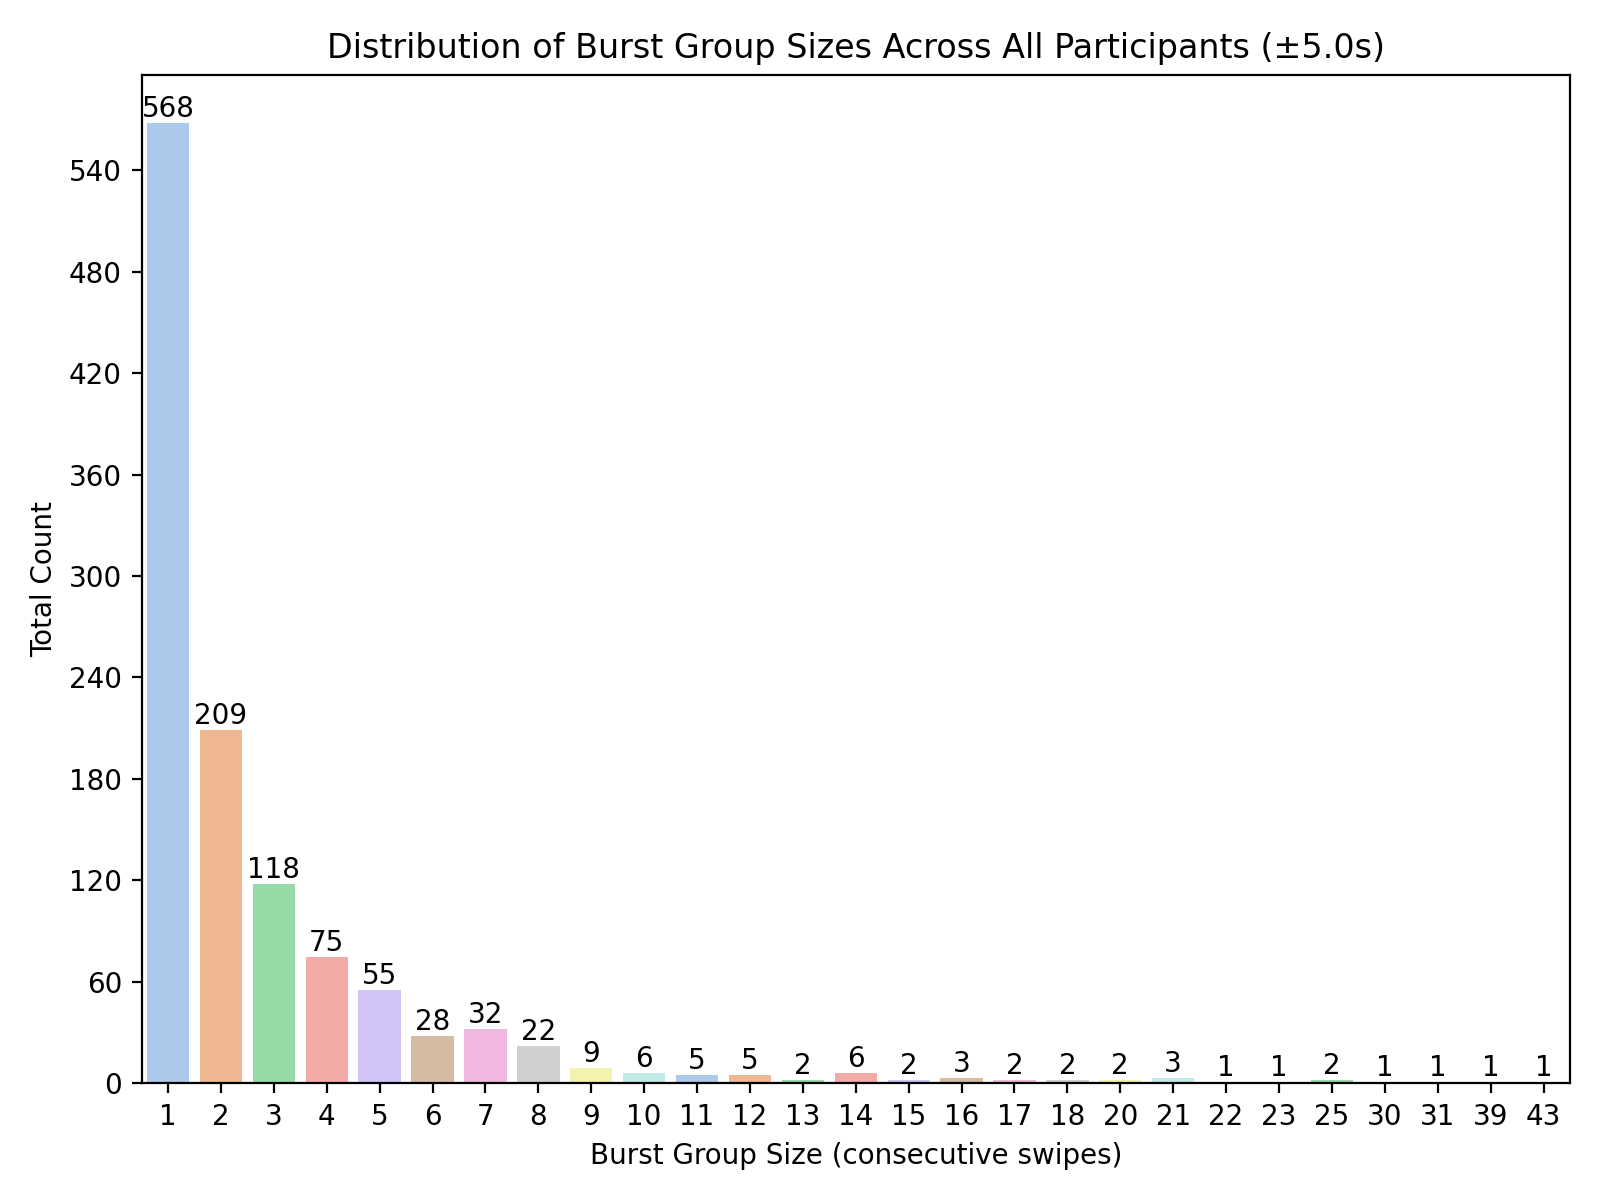
\includegraphics[width=\textwidth]{../05-12_data_analysis_and_results/runs/run_20260611_220844/viz/viz03/viz03.3.3_5s.png}
        \caption{Total burst group sizes across all participants (\(\pm5.0\)s window). The wider threshold computationally merges many normal swipes into larger burst blocks.}
        \label{fig:bursts_all_5s}
    \end{minipage}
\end{figure}


\section{The Engagement Index's Swipe-Prediction Performance}
\label{sec:results_engagement_index}

\subsection{Feature Importance and Neurophysiological Correlates}
\label{sec:results_feature_importance}

In Figure~\ref{fig:cohend_by_freq_band}, we observe that class separation, quantified via Cohen’s \(d\) as described in Section~\ref{sec:method_feature_separation_cohen_d}, is consistently stronger for several individual frequency bands (blue boxes) than for the conventional Engagement Index (red dotted line). In particular, the \(\alpha\)-band (8–13 Hz) achieves an effect size approximately 0.005 standard deviations higher than the Engagement Index, and the high-\(\gamma\) band (40–60 Hz), as the strongest candidate, exceeds it by more than 0.03 standard deviations. The Engagement Index — which combines three bands into a single scalar — itself reaches just above 0.02 and is therefore weaker in class separability than any of the individual frequency bands and the raw signal. This suggests that aggregating multiple bands into a single composite metric may dilute discriminative information that is more clearly expressed within specific, well-chosen frequency ranges.

Moreover, class separation reaches values above 0.04 only for a small subset of bands: the raw, broadband signal (without frequency decomposition), the \(\delta\) band (1–4 Hz), the low-\(\gamma\) band (30–40 Hz), and the high-\(\gamma\) band (40–60 Hz). These results indicate that both very low-frequency activity and specific \(\gamma\)-range oscillations carry comparatively strong discriminative structure for the SKIP versus STAY decision.

Taken together, these findings highlight three key points. First, individual frequency bands exhibit stronger class-separation capability than the conventional Engagement Index, suggesting that analyses based on raw or band-specific signals may be more informative than combined engagement metrics. Second, the raw broadband signal outperforms all separated bands except high \(\gamma\), which underscores the importance of preserving broadband information and motivates closer examination of high-\(\gamma\) activity in particular. Third, the pattern across bands follows a clear up–down–up trend: separability is high at low frequencies, drops to a minimum in the \(\alpha\) range (8–13 Hz), then rises to a global maximum in the high-\(\gamma\) range before decreasing again for very high \(\gamma\) frequencies (60–100 Hz). This systematic profile offers a frequency-resolved view of where discriminative information is concentrated in the EEG.
\begin{figure}[H]
    \centering
    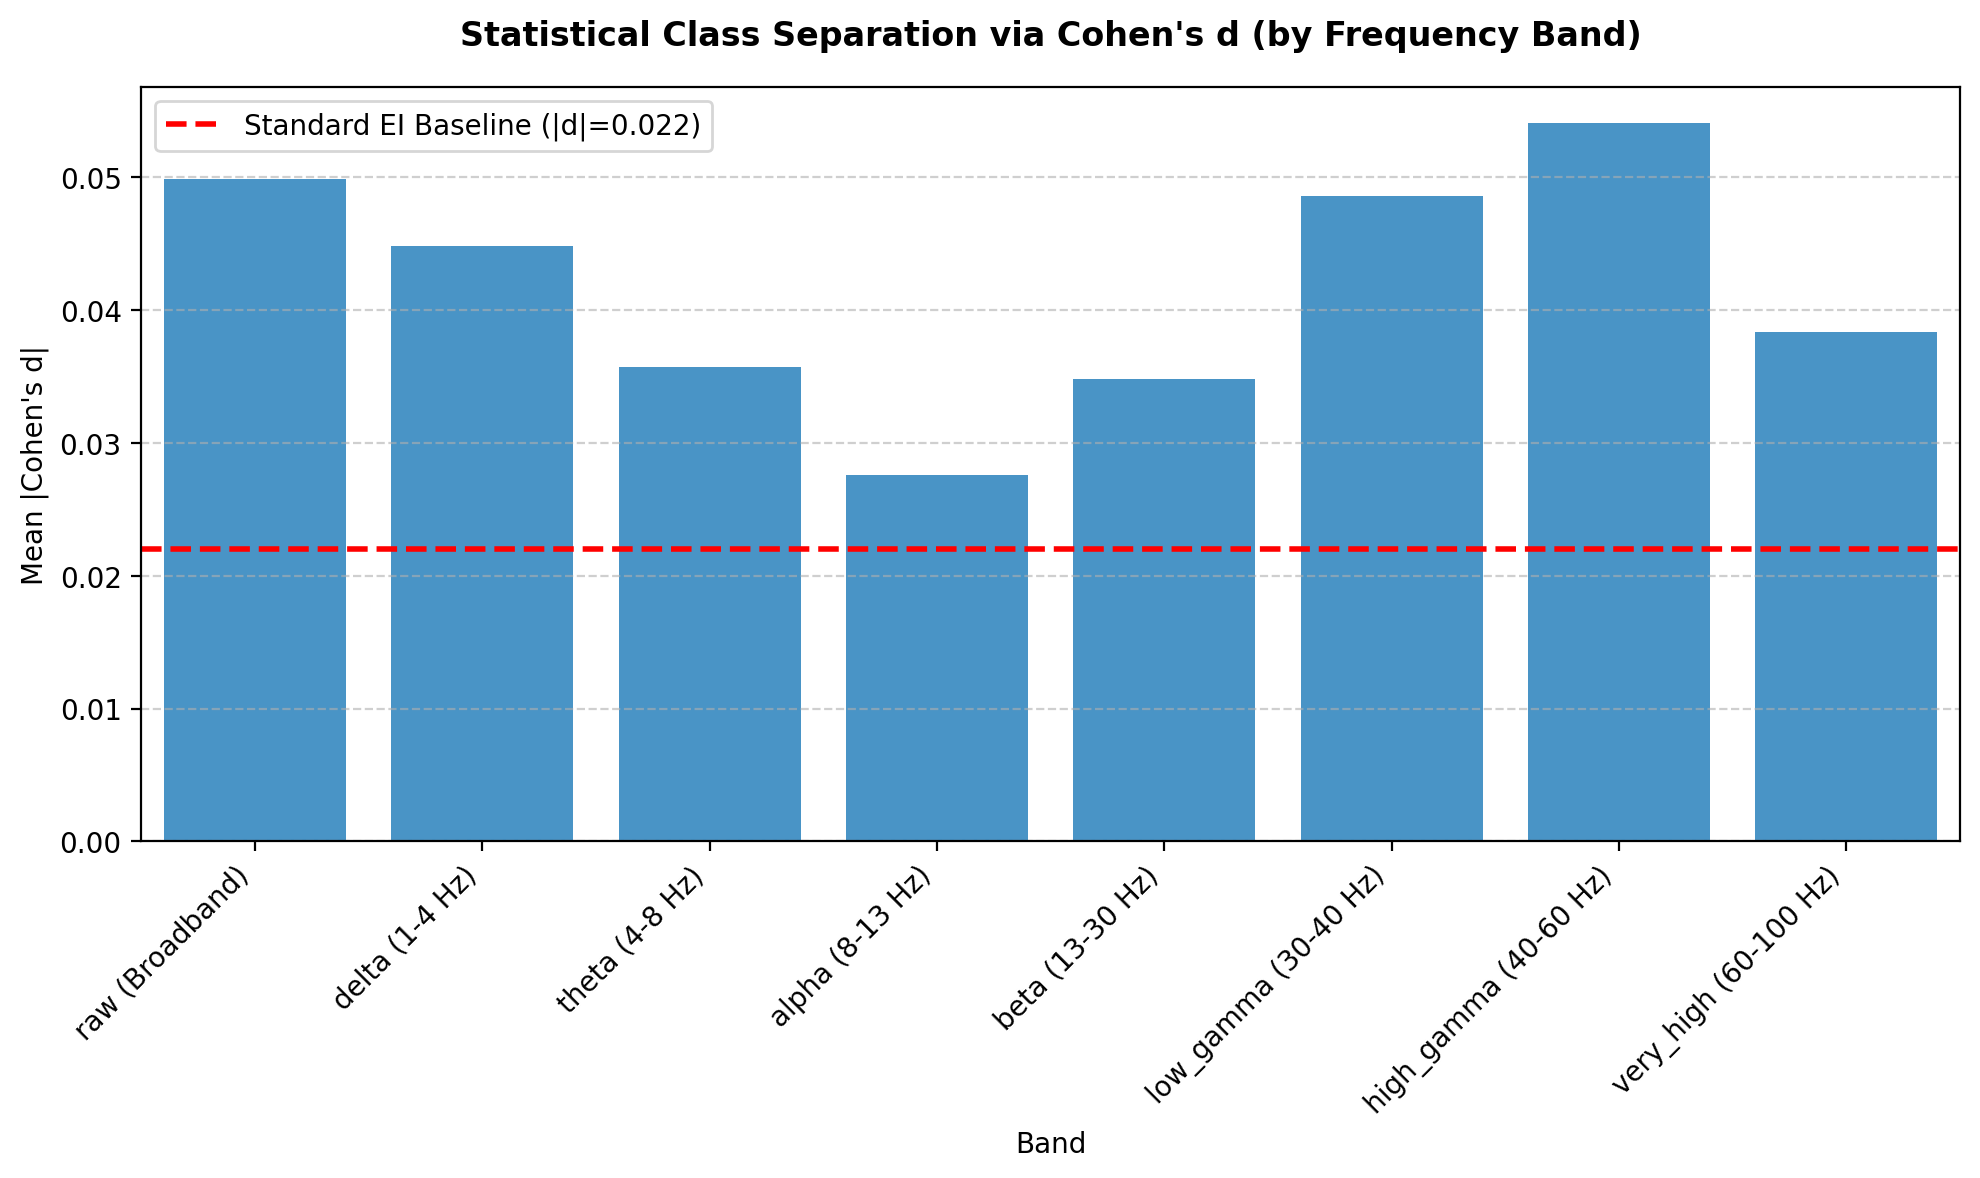
\includegraphics[width=\textwidth]{../05-12_data_analysis_and_results/runs/run_20260611_220844/viz/viz17_0.1.1_cohend_bands.png}
    \caption{Cohen's d effect size by frequency band.}
    \label{fig:cohend_by_freq_band}
\end{figure}

Similarly, Figure~\ref{fig:cohend_by_electrode} shows that separating the signal by electrode of origin — TP9, AF7, AF8, and TP10 — yields higher class separability than the conventional Engagement Index in all cases. The improvement ranges from just under 0.01 standard deviations for TP9 and AF8 to more than 0.03 standard deviations for AF7 and TP10. This suggests that distinguishing between individual brain regions provides more informative class separation than collapsing the signal into a single composite metric, and that the different electrodes contribute unequally to this discriminative task.

Moreover, the figure reveals a clear dominance of AF7 (left anterior frontal) and TP10 (right temporal pole) over TP9 (left temporal pole) and AF8 (right anterior frontal) in terms of Cohen’s \(d\). This pattern suggests that the frontal and right temporal regions contribute more strongly to the SKIP-versus-STAY separation than the left temporal pole and right anterior frontal regions, pointing to a potentially lateralized and region-specific neurophysiological signature of scrolling behavior.

AF7 (left anterior frontal) is the only electrode that outperforms the raw-data separation performance, and does so by just over 0.005 standard deviations, suggesting that this region may capture particularly salient discriminative information for the SKIP-versus-STAY distinction.

Potential systematic differences related to the recording electrodes cannot be excluded at this stage, as the data were collected using two different devices across the \(n = 25\) participants.

\begin{figure}[H]
    \centering
    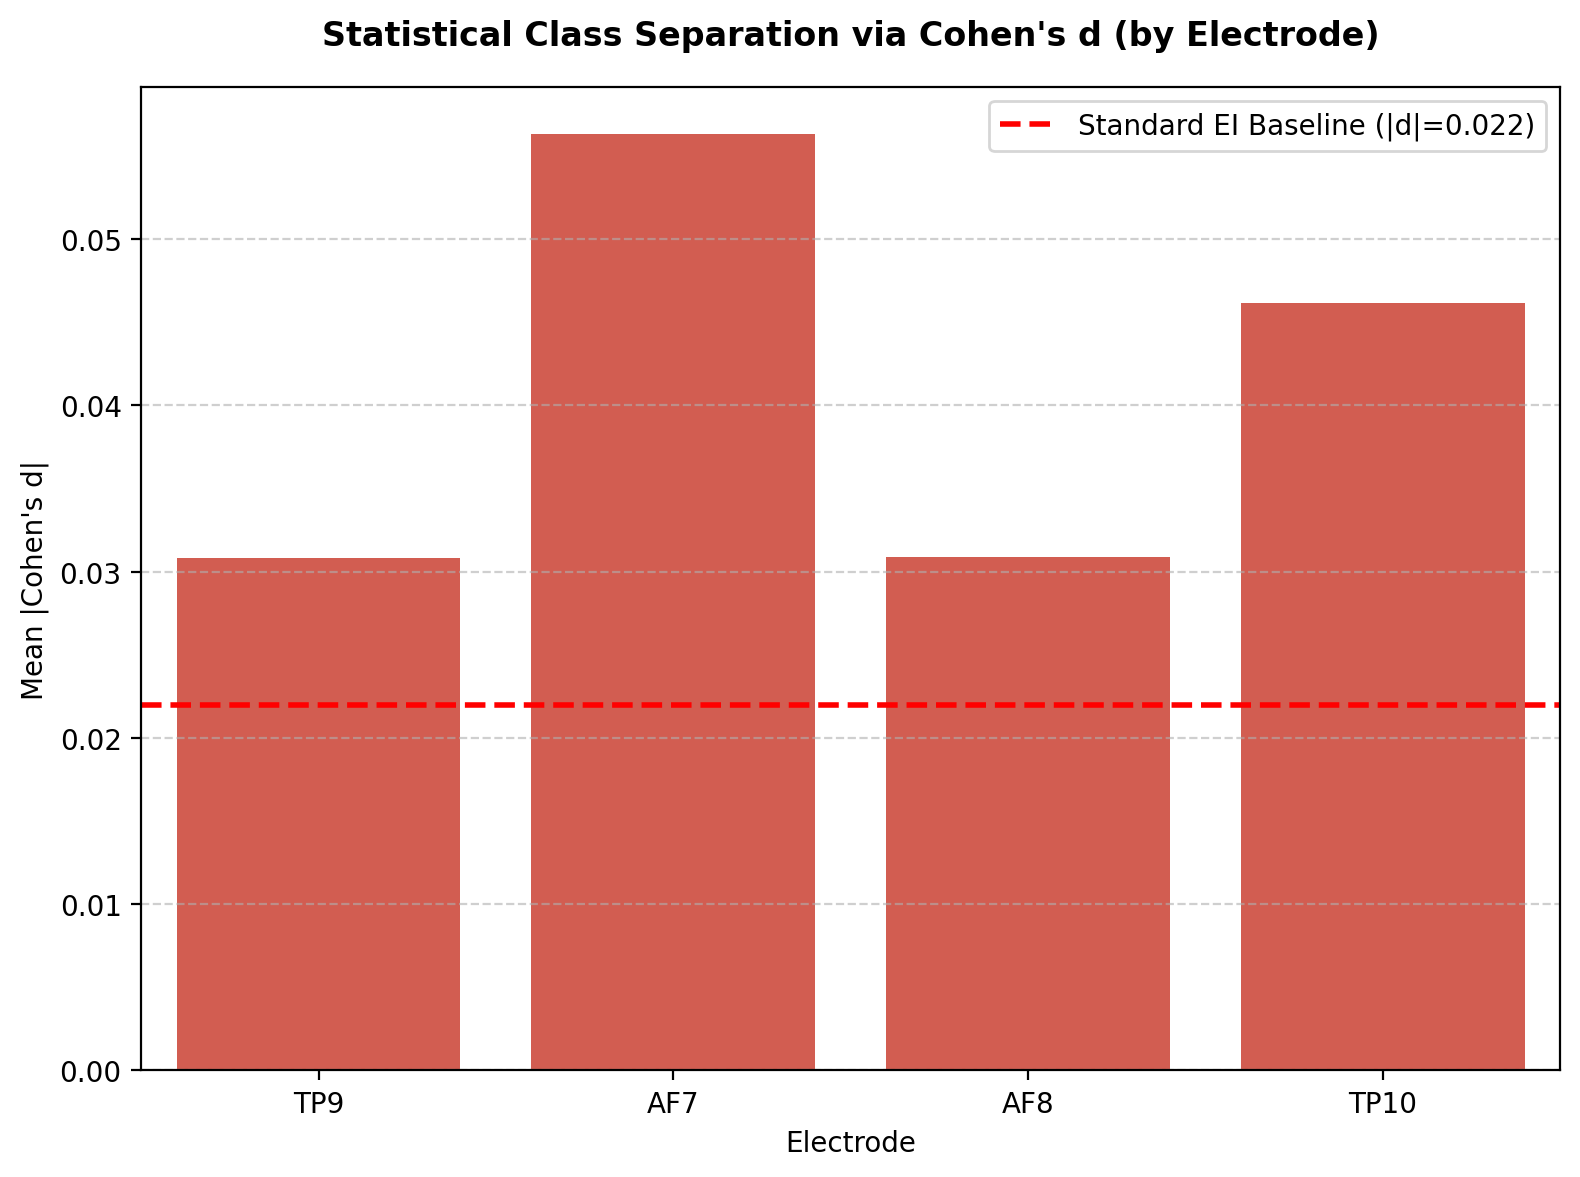
\includegraphics[width=\textwidth]{../05-12_data_analysis_and_results/runs/run_20260611_220844/viz/viz17_0.1.2_cohend_electrodes.png}
    \caption{Cohen's d effect size by electrode.}
    \label{fig:cohend_by_electrode}
\end{figure}

Figure~\ref{fig:cohend_by_stat_moment} shows that, among the statistical moments and related features considered, only a small subset exceeds the conventional Engagement Index by at least 0.01 standard deviations in terms of Cohen’s \(d\) class separation. These features are Hjorth activity, Hjorth mobility, the mean, the standard deviation, Hjorth complexity, and peak frequency. Taken together, this suggests that simple time-domain descriptors and Hjorth-derived measures retain meaningful discriminative information, but only for a limited number of feature types.

Furthermore, only two features - Hjorth complexity and peak frequency - outperform the raw-data class separation ability. This indicates that, while the unprocessed signal already contains substantial discriminative structure, certain higher-order descriptors can still extract additional information beyond the broadband signal alone.

Across the three feature families examined here - frequency bands, electrodes, and statistical moments/metrics - the statistical moments and metrics show the strongest overall class-separation performance. In particular, peak frequency stands out with a Cohen’s \(d\) of nearly 0.07, placing it almost 0.05 standard deviations above the conventional Engagement Index and nearly 0.02 standard deviations above the raw-data separation level. This makes peak frequency the strongest single feature in the present comparison and suggests that oscillatory structure within the signal may be especially informative for distinguishing between the two classes. At the same time, these findings should be interpreted cautiously, as the observed advantages are modest in absolute terms and may be influenced by dataset-specific factors.

\begin{figure}[H]
    \centering
    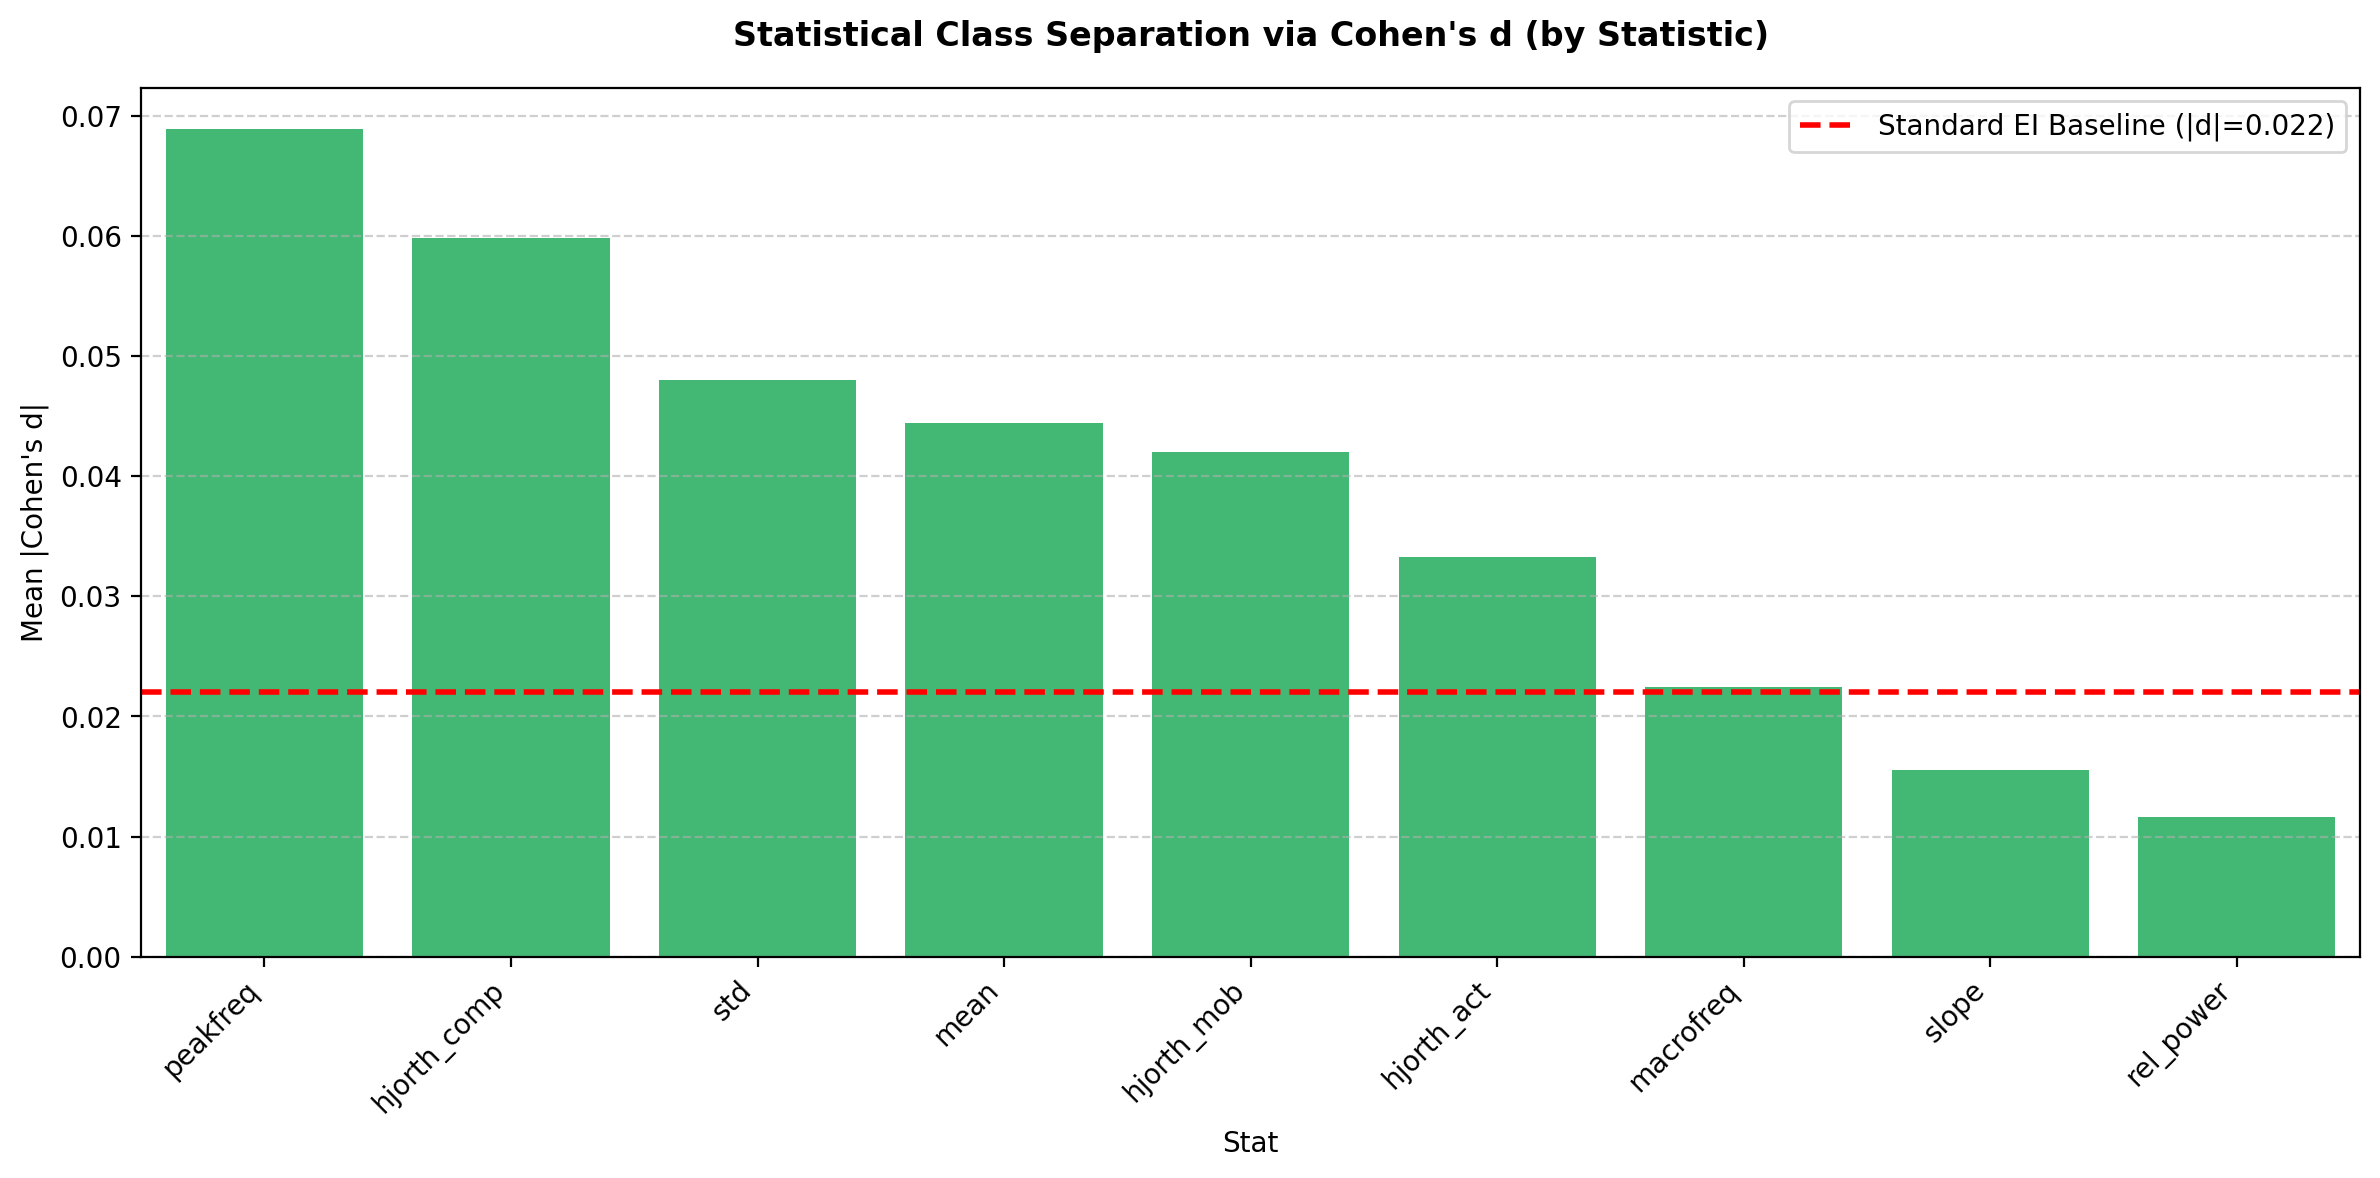
\includegraphics[width=\textwidth]{../05-12_data_analysis_and_results/runs/run_20260611_220844/viz/viz17_0.1.3_cohend_stats.png}
    \caption{Cohen's d effect size by statistical moment.}
    \label{fig:cohend_by_stat_moment}
\end{figure}

While the comparison of features up to this point has already provided informative detail, the highest level of resolution is reached when each parameter is specified individually: (i) electrode, (ii) band or raw signal, and (iii) statistic or metric. Table~\ref{tab:cohend_top_features} illustrates the value of this finer-grained perspective. In the preceding analyses, peak frequency emerged as the strongest class separator according to Cohen’s \(d\), when considering all bands and electrodes jointly. In those comparisons, the only variable under inspection was the parameter being held constant, while the remaining parameters varied across features. This resulted in aggregated Cohen’s \(d\) values for each parameter group, as shown in Figures~\ref{fig:cohend_by_freq_band}, \ref{fig:cohend_by_electrode}, \ref{fig:cohend_interactions}, and \ref{fig:cohend_by_stat_moment}. These results raise a natural question: are there individual features, defined across all three parameters, that exceed the currently best observed class-separation performance of peak frequency, at approximately \(0.07\)?

Table~\ref{tab:cohend_top_features} shows that such features do indeed exist. In fact, the top 30 features all outperform the peak-frequency result in terms of Cohen’s \(d\), indicating that a more specific feature definition can yield substantially stronger class separability. The strongest feature is TP10 raw standard deviation, with a Cohen’s \(d\) of \(0.196\), corresponding to an improvement of nearly tenfold over the conventional Engagement Index in terms of class separation.

This shows that class separability is not only determined by broad feature families such as frequency bands, electrodes, or statistical moments, but can increase substantially when the signal is described at the level of individual feature combinations. It further suggests that the conventional Engagement Index captures only part of the discriminative structure present in the data, whereas more specific features can reveal considerably stronger separation between classes. At the same time, these findings should be interpreted as evidence of dataset-specific predictive potential rather than as a universal hierarchy of feature importance.

% table of overall top features
% cohend_top_features
\begin{table}[H]
\centering
\begin{tabular}{llc}
\hline
Rank & Feature Name & $|$Cohen's $d|$ \\
\hline
1 & TP10 raw std & 0.196 \\
2 & AF7 high gamma mean & 0.168 \\
3 & AF7 high gamma hjorth mob & 0.145 \\
4 & AF7 delta hjorth comp & 0.141 \\
5 & AF8 delta peakfreq & 0.140 \\
6 & AF7 high gamma peakfreq & 0.139 \\
7 & TP9 delta hjorth comp & 0.137 \\
8 & TP9 delta peakfreq & 0.136 \\
9 & TP10 delta hjorth comp & 0.131 \\
10 & TP10 delta peakfreq & 0.130 \\
11 & AF7 theta hjorth comp & 0.129 \\
12 & AF7 raw std & 0.129 \\
13 & AF7 theta peakfreq & 0.124 \\
14 & AF7 low gamma hjorth comp & 0.124 \\
15 & AF7 delta peakfreq & 0.123 \\
16 & TP10 low gamma hjorth act & 0.119 \\
17 & AF8 high gamma mean & 0.119 \\
18 & AF7 low gamma mean & 0.118 \\
19 & AF7 beta mean & 0.115 \\
20 & AF8 delta hjorth comp & 0.115 \\
21 & TP10 low gamma std & 0.114 \\
22 & TP10 high gamma hjorth mob & 0.110 \\
23 & AF7 very high mean & 0.109 \\
24 & TP10 beta hjorth act & 0.108 \\
25 & TP9 theta peakfreq & 0.103 \\
26 & TP9 high gamma std & 0.103 \\
27 & TP10 beta std & 0.100 \\
28 & AF8 theta peakfreq & 0.100 \\
29 & AF7 beta hjorth comp & 0.100 \\
30 & TP9 high gamma hjorth act & 0.098 \\
\hline
\end{tabular}
\caption{Top 30 Features by Separation ($|$Cohen's $d|$).}
\label{tab:cohend_top_features}
\end{table}

For all features, Figure~\ref{fig:cohend_interactions} shows Cohen’s \(d\) values sorted jointly by frequency band and electrode. For the raw, broadband signal (no frequency filtering), the top feature “TP10 raw std” clearly appears as the global peak in the visualization. Overall, similar trends to the previous figures can be observed, but the combined view makes electrode–band interactions more apparent. In particular, there is a pronounced spike in class-separation performance for the broadband signal at TP10 and AF7.

Moreover, the AF7 electrode stands out by exhibiting a clear upward trend in Cohen’s \(d\) from the \(\alpha\) band (8–13 Hz) through \(\beta\) (13–30 Hz) to low \(\gamma\) (30–40 Hz), followed by a plateau across the broader \(\gamma\) range (30–100 Hz; low, high, and very high \(\gamma\)) with a slight decline toward the highest frequencies. The peak for AF7 lies in the low-\(\gamma\) band (30–40 Hz), where its class-separation ability is highest. This enhanced separability for the SKIP-versus-STAY distinction at AF7 (left anterior frontal), particularly in the \(\gamma\) and high-\(\gamma\) range (30–100 Hz), may suggest that left anterior frontal oscillatory activity in this frequency range is especially sensitive to the neural processes that differentiate sustained engagement from disengagement decisions in this task. These interpretations should, however, be viewed as preliminary and require replication in independent datasets.

Furthermore, the superior class-separation ability of the TP10 broadband signal, relative to TP10’s performance within individual frequency bands, suggests that discriminative information may extend beyond the conventional 1–100 Hz decomposition. This could indicate that additional signal components, including potential artifacts such as electromyographic activity from jaw movements, contribute to the SKIP-versus-STAY separation alongside, or in some cases instead of, purely neural activity. These possibilities highlight the need for careful artifact characterization and control in future work.

\begin{figure}[H]
    \centering
    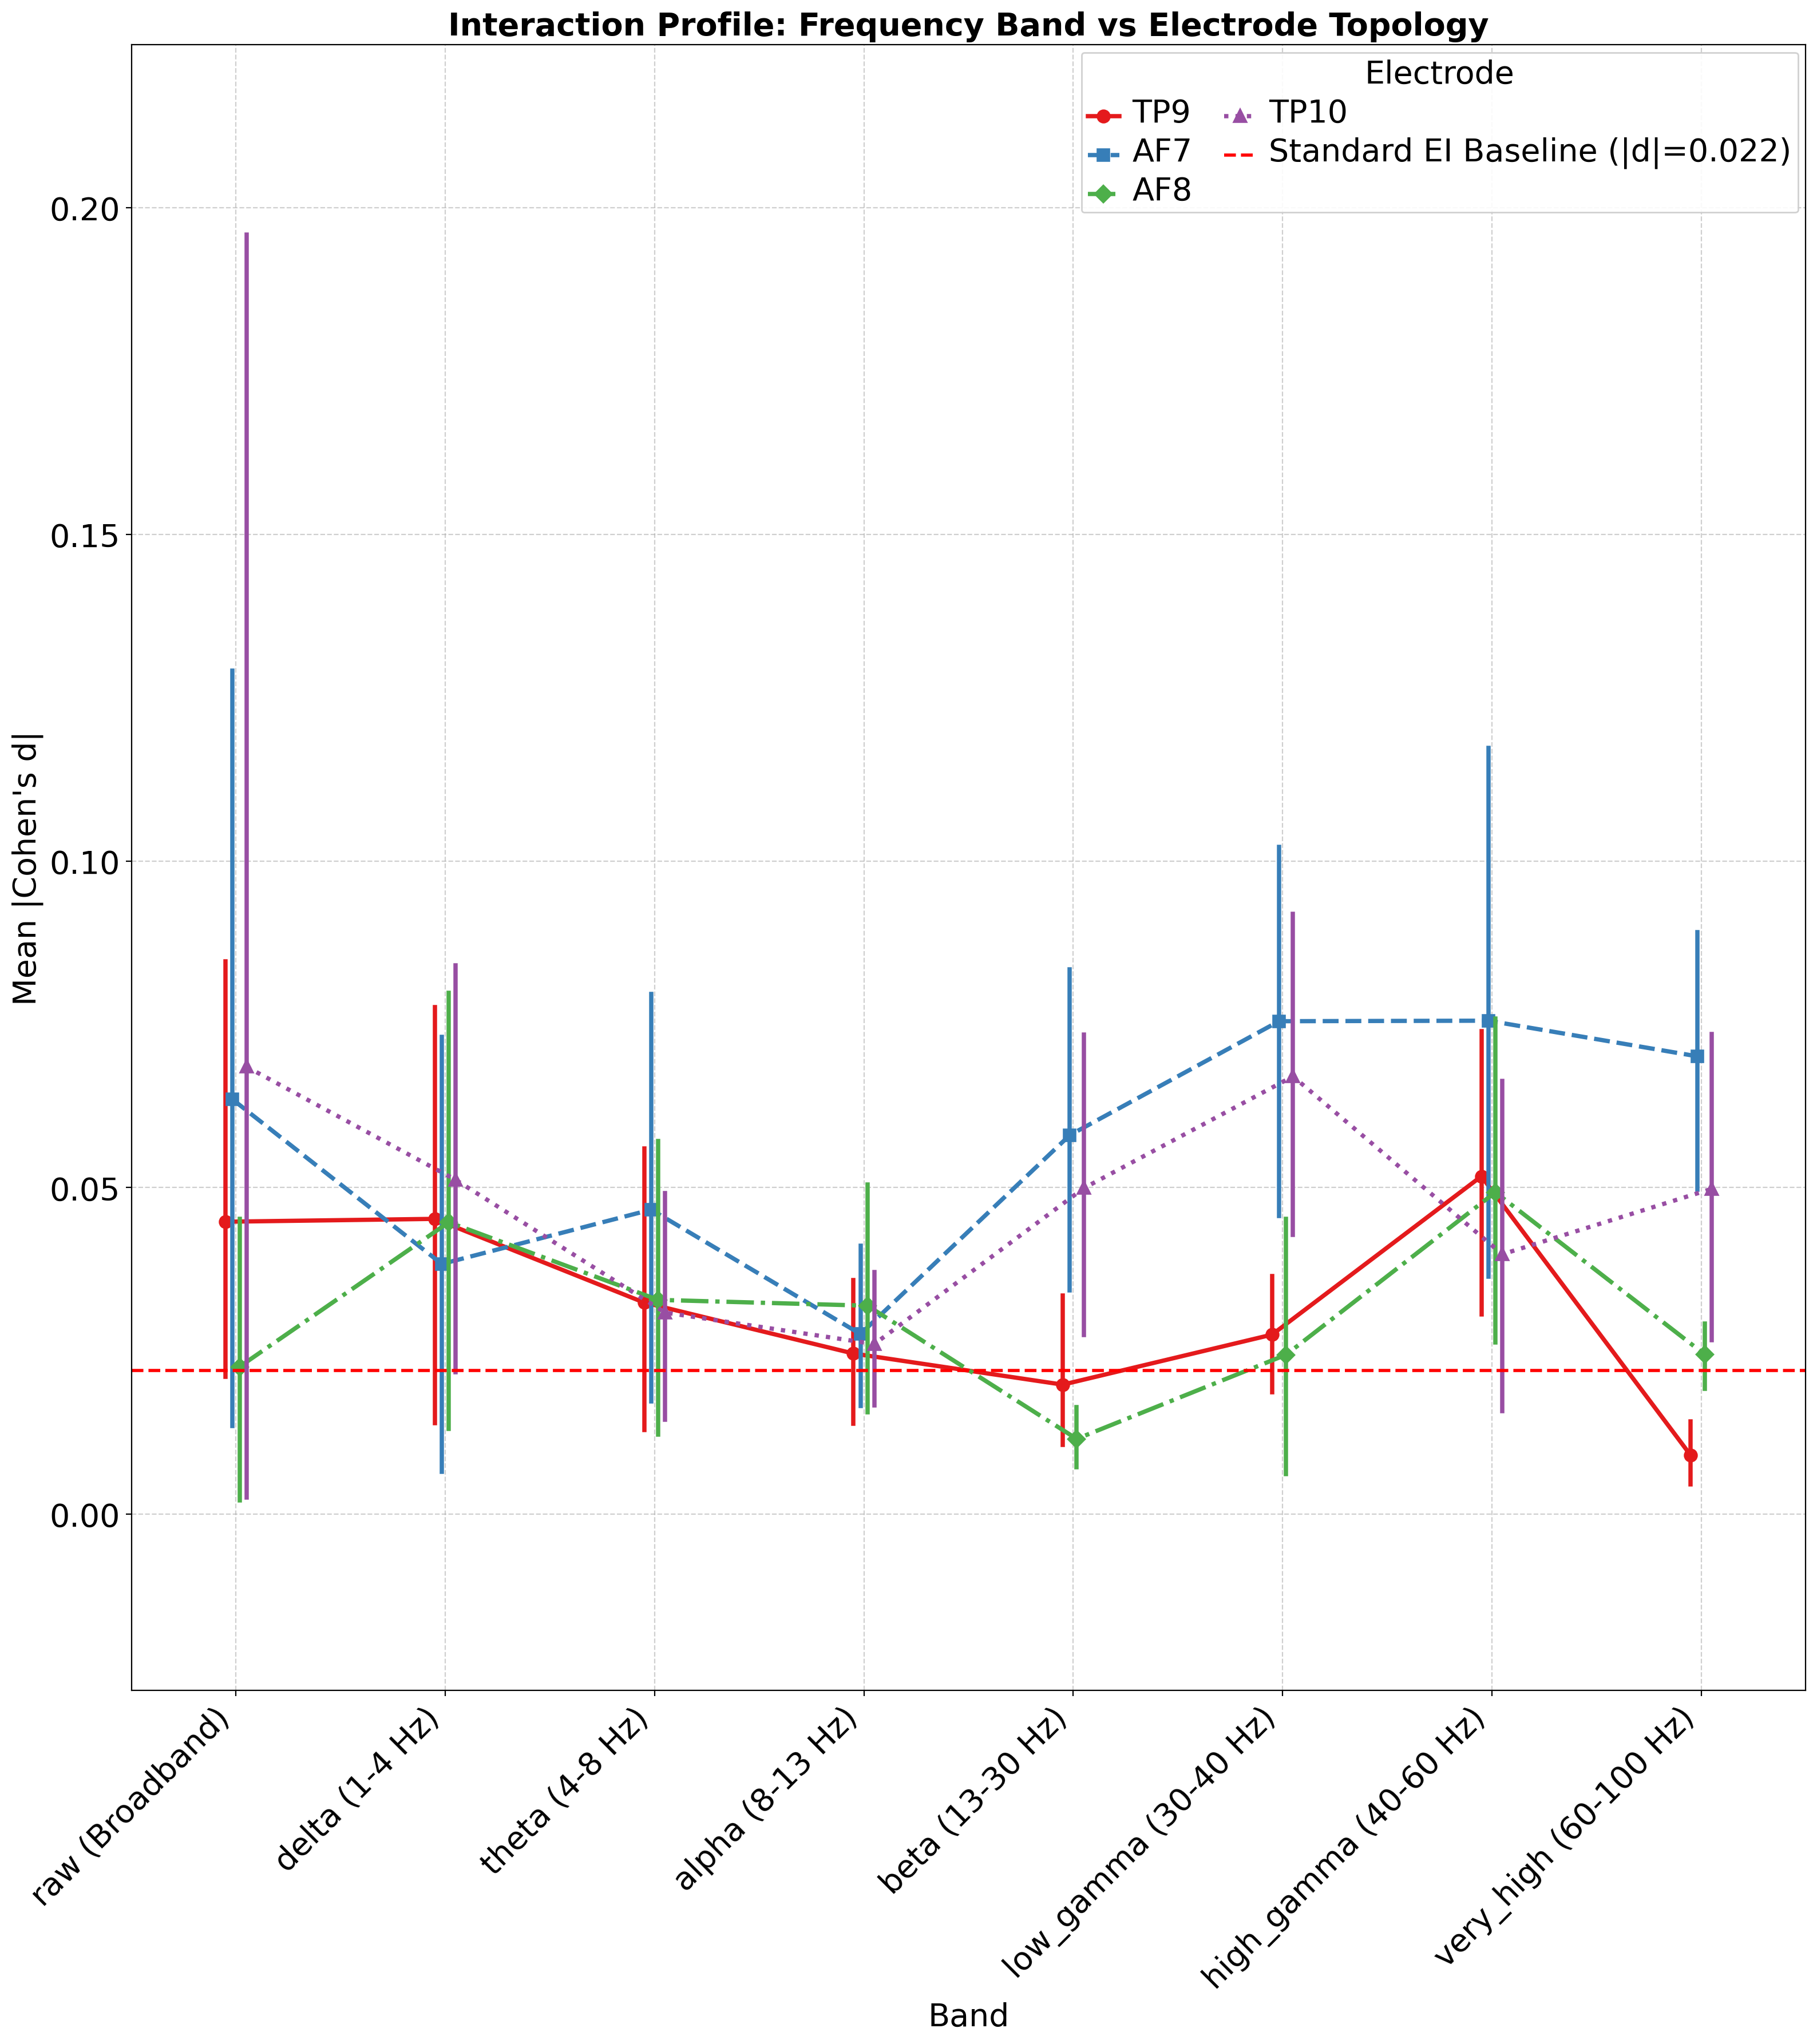
\includegraphics[width=\textwidth]{../05-12_data_analysis_and_results/runs/run_20260611_220844/viz/viz17_0.1.4_cohend_interactions.png}
    \caption{Cohen's d effect size interactions.}
    \label{fig:cohend_interactions}
\end{figure}

As shown in Figure~\ref{fig:cohend_top_features_2} the top features were selected for each category: i) overall top feature \#1, ii) overall top feature \#2, iii) top \#1 feature of top band, iv) top \#1 feature of top electrode, v) top \#1 feature of top statistic/metric.

The feature "TP10 raw std" (|d| = 0.20) is placed for i) feature \#1, whereas "AF7 high gamma mean" (|d| = 0.17) simultaneously represents all 3 categories ii), iii) and iv). "AF8 delta peakfreq" (|d| = 0.14) feature takes the place of category v), which is the \#1 feature amongst the top statistics, namely the Peak-frequency.

\begin{figure}[H]
    \centering
    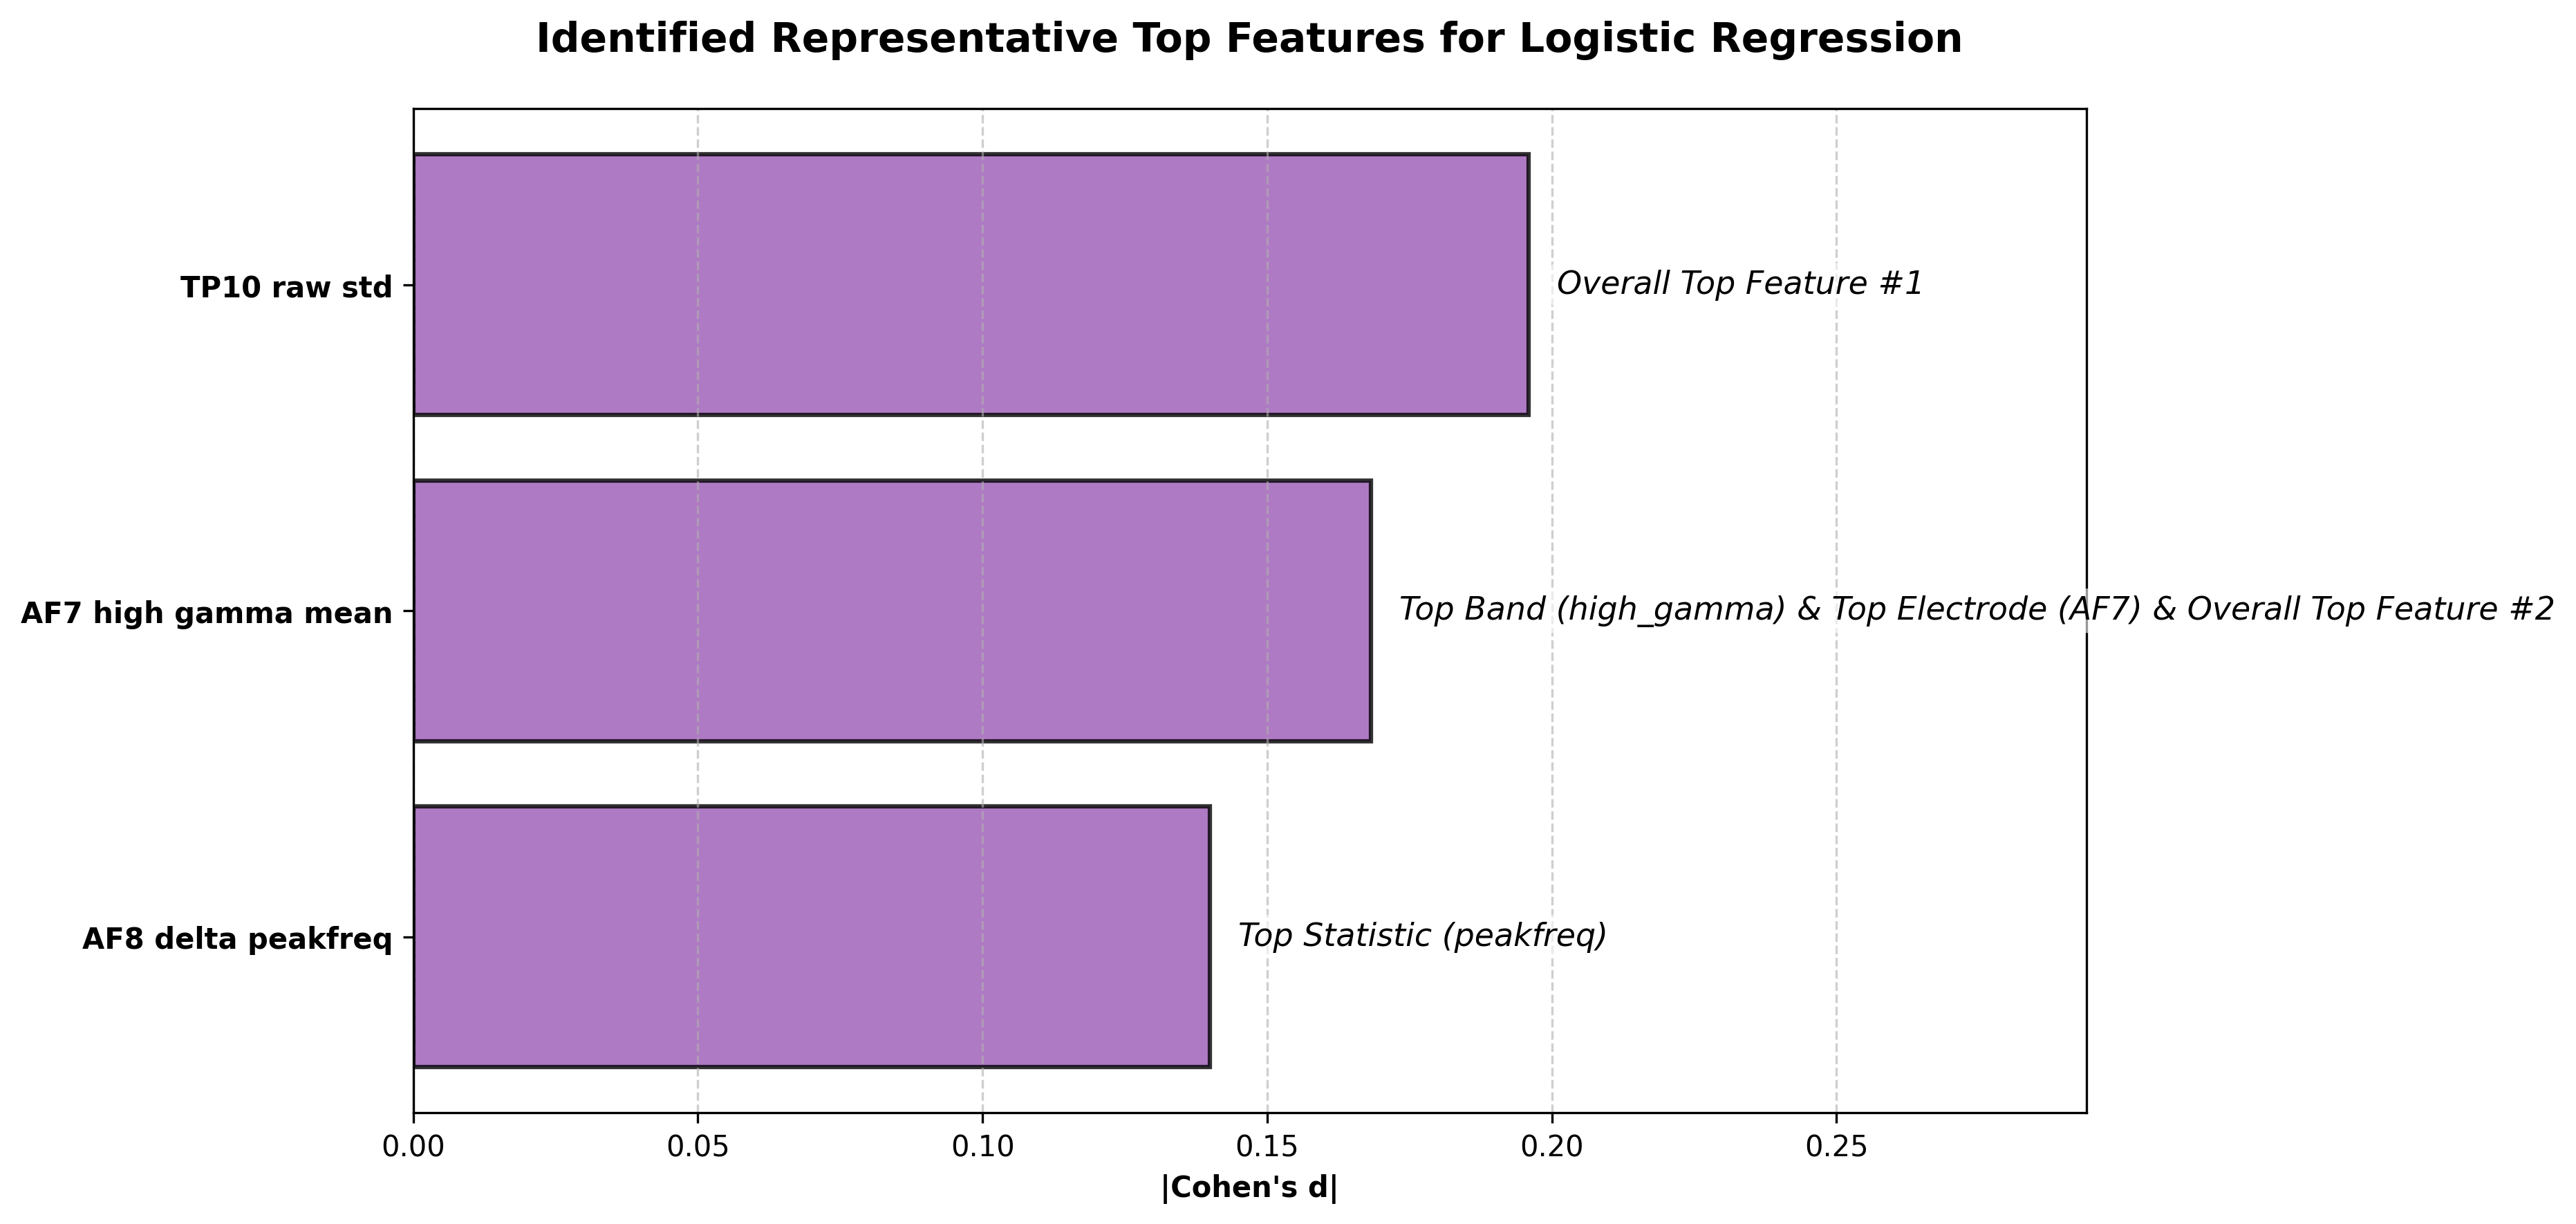
\includegraphics[width=\textwidth]{../05-12_data_analysis_and_results/runs/run_20260611_220844/viz/viz17_4_identifying_top.png}
    \caption{Identifying top predictive features.}
    \label{fig:cohend_top_features_2}
\end{figure}

\subsection{Engagement Index Model Performance and Benchmark Comparison}
\label{sec:results_model_performance}

The modeling framework described in Section~\ref{sec:method_baselines_and_logistic_regression} was used to evaluate whether the engineered EEG features could predict \texttt{SKIP} versus \texttt{STAY} behavior beyond chance and beyond the conventional Engagement Index. First, a coin-flip baseline established the empirical chance level. Second, the Engagement Index was evaluated as a one-dimensional logistic regression baseline. Third, the strongest features identified in Section~\ref{sec:results_feature_importance} were tested in isolated logistic regression models to assess whether they could improve predictive performance beyond the baseline models.

To evaluate predictive performance, standard classification metrics were computed as described in Section~\ref{sec:method_metrics_and_significance}. In particular, Accuracy, Precision, Recall, and the F\(_1\)-score were calculated for each cross-validation fold, separately for both classes via one-vs-rest evaluation. The F\(_1\)-score served as the primary metric because it balances Precision and Recall and is therefore more informative than Accuracy under the present class structure.

Statistical significance was assessed using the Wilcoxon signed-rank test, as outlined in Section~\ref{sec:method_metrics_and_significance}. The coin-flip baseline serves as the reference for chance-level performance, whereas the Engagement Index is used as the clinical baseline for subsequent comparisons. Performance is reported both for the intra-subject evaluation setting, in which models were trained and tested within the same participant, and for the inter-subject evaluation setting, in which models were generalized across participants. The corresponding results are shown in Table~\ref{tab:metrics_1_intra} and Table~\ref{tab:metrics_1_inter}, respectively. In these tables, green values indicate metrics that are not only significantly different from the baseline, but also significantly higher than the baseline, thus reflecting genuine performance gains rather than mere statistical deviation.

At the inter-subject level shown in Table~\ref{tab:metrics_1_inter}, the Engagement Index logistic regression yields a statistically significant improvement over the coin-flip baseline only for \texttt{STAY} as the positive class. The most prominent effect is Recall, which rises to 89.2\% compared with 51.7\% for the coin-flip baseline. This indicates that the model is highly sensitive to \texttt{STAY} windows and rarely misses them, but it does not necessarily imply balanced or reliable class discrimination on its own. In fact, high Recall in combination with only moderate F\(_1\)-scores suggests a strong tendency to capture the majority of \texttt{STAY} instances while still leaving room for false positives, meaning that the model may be better at recognizing sustained engagement than at sharply distinguishing it from disengagement.

The corresponding F\(_1\)-scores provide a more nuanced interpretation. At 62.0\% for training and 62.5\% for testing, the model performs above chance and remains relatively stable across folds, which argues against severe overfitting in the inter-subject setting. However, the gain over the coin-flip baseline is modest in absolute terms, especially when viewed alongside the comparatively large improvement in Recall. This combination suggests that the Engagement Index carries some predictive structure, but that this structure is unevenly distributed across metrics: it may identify \texttt{STAY} behavior reasonably well, yet it does not provide a uniformly strong decision boundary between the two classes.

Importantly, these results also clarify what the Engagement Index can and cannot do in this dataset. It appears capable of capturing a limited but real signal related to sustained engagement, particularly for \texttt{STAY}, but it is not sufficient as a standalone descriptor of the full SKIP-versus-STAY decision. The fact that the model improves clearly in Recall while remaining only moderately strong in F\(_1\)-score raises a central interpretive question: does the Engagement Index reflect a broad engagement-related tendency, or is it primarily sensitive to a subset of windows that are easier to classify as \texttt{STAY}? This ambiguity motivates the next analytical step in Section \ref{sec:results_alternative_index}, namely to examine which specific features, electrodes, and frequency ranges contribute more directly to class separability and whether they offer a more interpretable explanation as an 'Alternative Index' over the aggregate Engagement Index. In that sense, the present numbers do not merely indicate performance; they identify the precise limitation of the baseline and justify moving toward feature-level interpretation and model comparison.

% CF vs EI - intra - per participant
% metrics_1_intra
\begin{table}[ht]
\centering
\begin{tabular}{lccc}
\hline
Metric & Coin Flip & \multicolumn{2}{c}{EI LR} \\\\
 & Val & Val & Sig \\\\
\hline
F1 Train (STAY) & 50.6\% & \textcolor{green}{53.8\%} & TRUE \\\\
F1 Test (STAY) & 52.4\% & \textcolor{green}{50.9\%} & TRUE \\\\
Precision (STAY) & 50.1\% & \textcolor{green}{49.1\%} & TRUE \\\\
Recall (STAY) & 55.0\% & \textcolor{green}{52.9\%} & TRUE \\\\
F1 Train (SKIP) & 49.4\% & 49.6\% & FALSE \\\\
F1 Test (SKIP) & 47.5\% & 46.9\% & FALSE \\\\
Precision (SKIP) & 50.1\% & \textcolor{green}{48.9\%} & TRUE \\\\
Recall (SKIP) & 45.2\% & 45.1\% & FALSE \\\\
\hline
\end{tabular}
\caption{Step 1: EI vs Coin Flip. Significance tested using Wilcoxon signed-rank test against Coin Flip (two-sided, $\alpha=0.05$, N=25).}
\label{tab:metrics_1_intra}
\end{table}

% CF vs EI - inter - cross participant
% metrics_1_inter
\begin{table}[H]
\centering
\begin{tabular}{lccc}
\hline
Metric & Coin Flip & \multicolumn{2}{c}{EI LR} \\\\
 & Val & Val & Sig \\\\
\hline
F1 Train (STAY) & 50.3\% & \textcolor{green}{62.0\%} & TRUE \\\\
F1 Test (STAY) & 50.8\% & \textcolor{green}{62.5\%} & TRUE \\\\
Precision (STAY) & 49.9\% & 49.4\% & FALSE \\\\
Recall (STAY) & 51.7\% & \textcolor{green}{89.2\%} & TRUE \\\\
F1 Train (SKIP) & 49.6\% & 20.6\% & TRUE \\\\
F1 Test (SKIP) & 48.9\% & 10.7\% & TRUE \\\\
Precision (SKIP) & 49.9\% & 23.5\% & TRUE \\\\
Recall (SKIP) & 48.0\% & 9.6\% & TRUE \\\\
\hline
\end{tabular}
\caption{Step 1 (Inter-Subject): EI vs Coin Flip. Significance tested using Wilcoxon signed-rank test against Coin Flip (two-sided, $\alpha=0.05$, N=25).}
\label{tab:metrics_1_inter}
\end{table}

When assessing the individual participants' performance in the cross-participant model setting, as shown in Figure~\ref{fig:ei_vs_cf_inter_significance_heatmap}, the pattern further supports the interpretation that \texttt{STAY} events are systematically and significantly easier for the Engagement Index to recognize than \texttt{SKIP} events are to detect reliably. This asymmetry suggests that the model captures a broad tendency toward sustained engagement, but lacks equally strong sensitivity to the more transient disengagement-related decision signal.

% \input{../05-12_data_analysis_and_results/runs/run_20260611_220844/viz/viz17_2_inter_significance_thesis_paragraph.tex}

\begin{figure}[H]
    \centering
    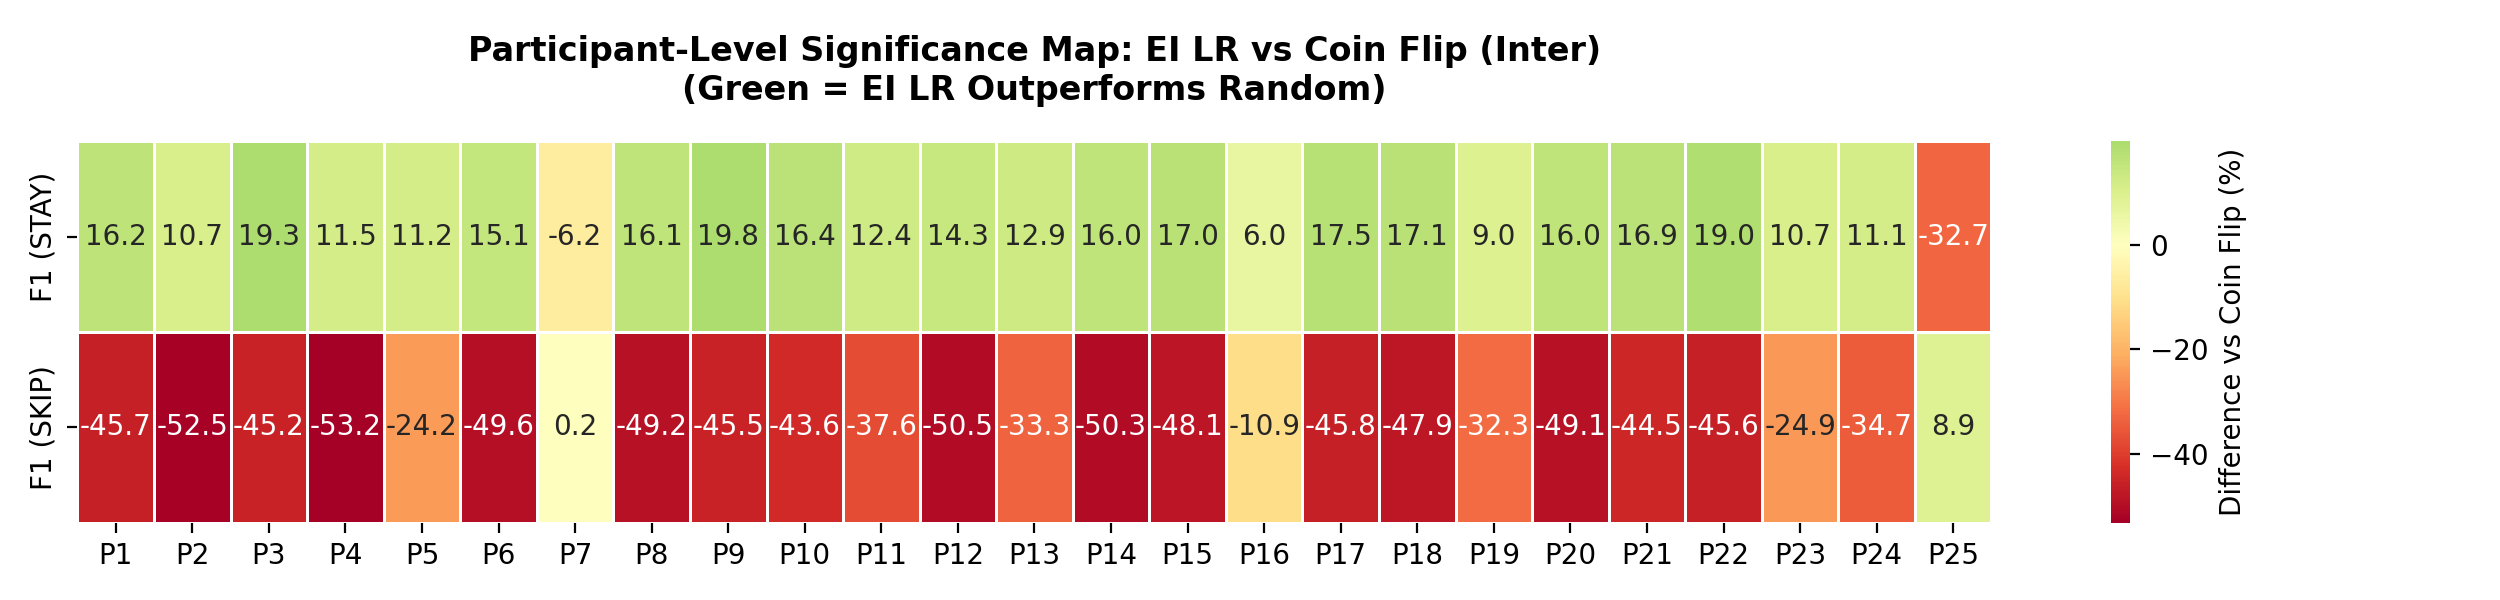
\includegraphics[width=\textwidth]{../05-12_data_analysis_and_results/runs/run_20260611_220844/viz/viz17_2_inter_significance.png}
    \caption{Inter-subject significance heatmap comparing F\(_1\)-test performance of the Engagement Index and the coin-flip baseline for \texttt{SKIP} and \texttt{STAY} as positive classes.}
    \label{fig:ei_vs_cf_inter_significance_heatmap}
\end{figure}

\iffalse
To rigorously determine whether a predictive model meaningfully outperforms the random baseline (Coin Flip) or the standard reference (Engagement Index, EI), statistical significance was evaluated using the Wilcoxon signed-rank test. Unlike standard parametric tests (such as the paired t-test) which assume performance metrics are normally distributed, the Wilcoxon test is a non-parametric alternative. This makes it particularly robust for highly individual, small-sample physiological data such as EEG ($N=25$ participants).

Rather than comparing a single aggregated mean across the dataset, the test utilizes paired metrics derived from the 25 participant-specific evaluations, where an individualized model is trained and tested exclusively on each participant's own data splits. The procedure calculates the difference in performance (e.g., F1-score) between the evaluated model and the baseline for each specific participant. By ranking the absolute values of these differences and applying their original signs, the test evaluates whether the median of the differences is significantly shifted from zero. This participant-level comparison ensures that a model only achieves significance if it consistently outperforms the baseline across the majority of individuals, preventing a scenario where exceptional performance on a few participants artificially inflates the overall mean. A visual representation of these paired differences across all participants is provided in the significance heatmap (see Figure~\ref{fig:viz17_2_intra_significance}), which color-codes the exact performance gap for each participant.

The algorithm employs a two-sided Wilcoxon test with a standard significance threshold ($\alpha = 0.05$). Because a two-sided test detects significant differences in either direction (meaning the model could be significantly better \textit{or} significantly worse than the baseline), a directional validation check is applied post-hoc. A model's performance is deemed statistically significantly superior only if it meets two strict conditions: first, the test must yield $p < 0.05$; second, the arithmetic mean of the model's scores across all participants must be strictly greater than the baseline's mean. The results of this rigorous evaluation, including the final validated significance flags for each metric, are summarized in Table~\ref{tab:metrics_1_intra}. Furthermore, the test assumes that metric distributions are independent between participants, but appropriately treats models evaluated on the identical set of participant features as dependent, paired samples. Zero-differences (ties) are naturally handled by standard removal from the ranking process.

\fi

\iffalse
\begin{figure}[H]
    \centering
    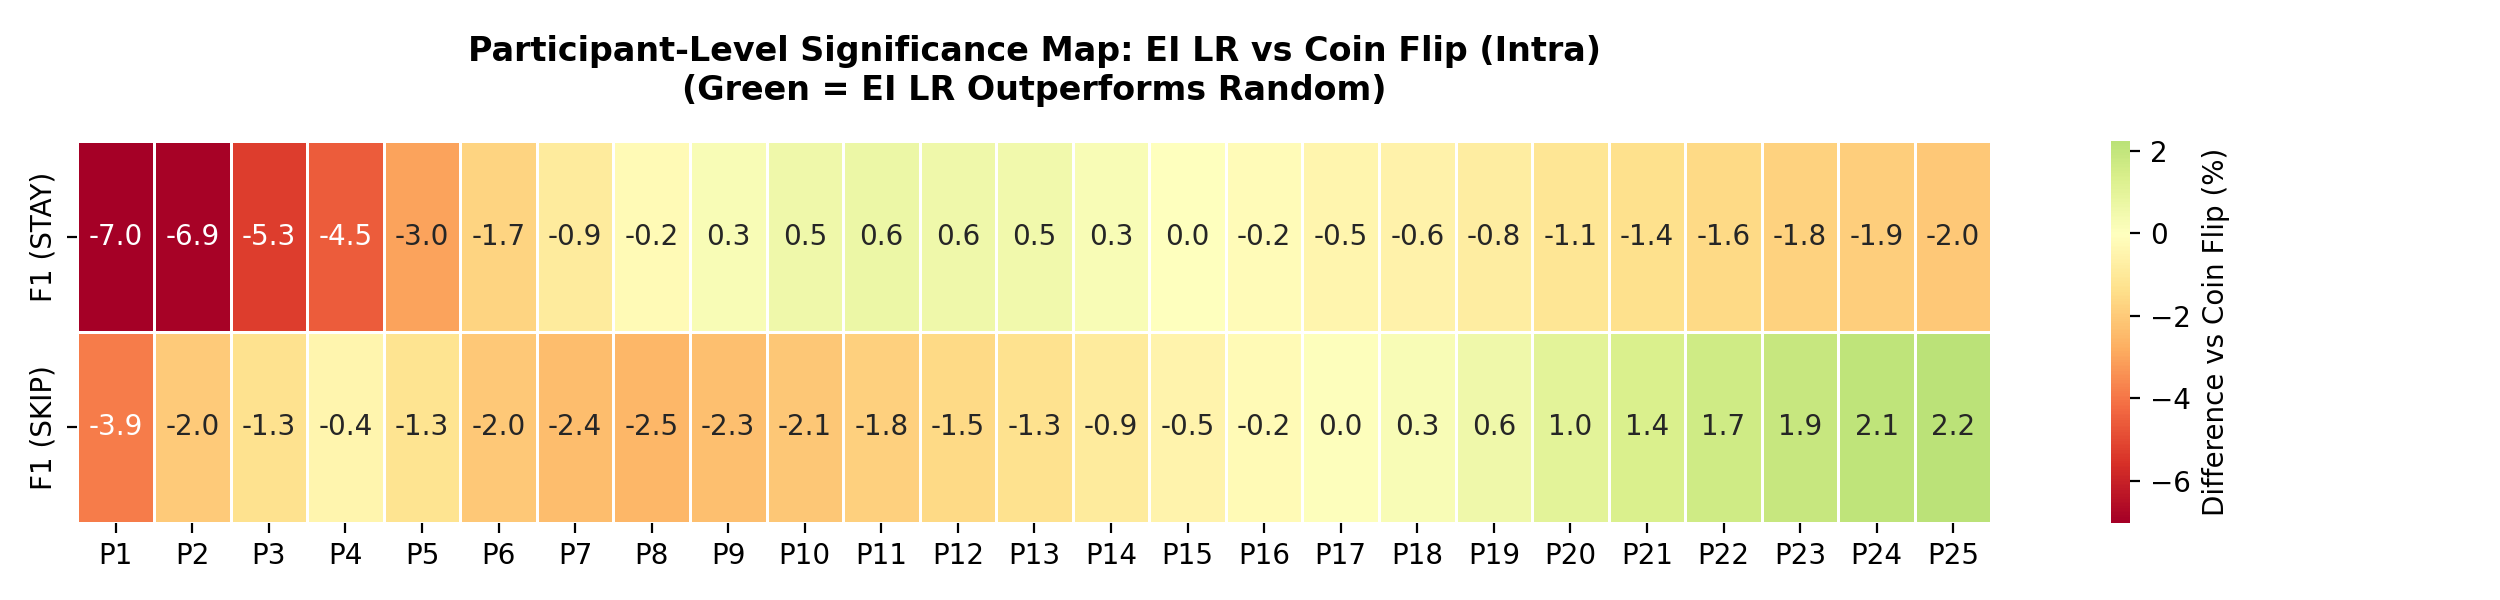
\includegraphics[width=\textwidth]{../05-12_data_analysis_and_results/runs/run_20260611_220844/viz/viz17_2_intra_significance.png}
    \caption{Intra-subject significance analysis.}
    \label{fig:ei_vs_cf_intra_significance_heatmap}
\end{figure}
\fi

\subsection{Alternative Index Exploration}
\label{sec:results_alternative_index}

Alternative Index Exploration entails the evaluation of individual features, informed by the 3 identified best-at-separating classes via Cohen's d top-features in Section \ref{sec:results_feature_importance}, namely "TP10 raw std", "AF7 high gamma mean" and "AF8 delta peakfreq", which are fed into a Logarithmic Regression model, and compared directly to the Engagement Index Logarithmic Regression Model performance from the previous step in Section \ref{sec:results_model_performance}.

\subsubsection{Intra-Subject (Per-Participant Level)}

The performance of TP10 raw standard deviation relative to the Engagement Index is shown in Table~\ref{tab:metrics_5_intra_3}. At the intra-subject level, the only significant improvement is observed for F\(_1\)-train with \texttt{SKIP} as the positive class, where TP10 raw standard deviation reaches 53.6\% compared with 49.6\% for the Engagement Index. Because this advantage does not carry over to the test set, it should be interpreted cautiously and is more consistent with participant-specific overfitting than with robust predictive structure. Nevertheless, the result is still informative: it suggests that raw signal variability at TP10 may contain class-related information that the Engagement Index does not capture, even if that information is not stable enough to generalize within participants.

% \ref{tab:metrics_5_intra_3}
% TP10 raw std
\begin{table}[H]
\centering
\begin{tabular}{lccc}
\hline
Metric & EI LR & \multicolumn{2}{c}{TP10 raw std} \\\\
 & Val & Val & Sig \\\\
\hline
F1 Train (STAY) & 53.8\% & 52.4\% & TRUE \\\\
F1 Test (STAY) & 50.9\% & 49.3\% & TRUE \\\\
Precision (STAY) & 49.1\% & 48.2\% & TRUE \\\\
Recall (STAY) & 52.9\% & 50.4\% & TRUE \\\\
F1 Train (SKIP) & 49.6\% & \textcolor{green}{52.6\%} & TRUE \\\\
F1 Test (SKIP) & 46.9\% & 46.8\% & FALSE \\\\
Precision (SKIP) & 48.9\% & 47.9\% & TRUE \\\\
Recall (SKIP) & 45.1\% & 45.7\% & FALSE \\\\
\hline
\end{tabular}
\caption{Step 5 (Intra): Proposed Feature (TP10 raw std) vs EI. Significance tested using Wilcoxon signed-rank test against EI (two-sided, $\alpha=0.05$, N=25).}
\label{tab:metrics_5_intra_3}
\end{table}

The performance of AF7 high-\(\gamma\) mean relative to the Engagement Index is shown in Table~\ref{tab:metrics_5_intra_1}. Here, several small but significant improvements emerge: Precision for \texttt{STAY} rises to 49.9\% from 49.1\%, F\(_1\)-train for \texttt{SKIP} increases to 52.9\% from 49.6\%, and Precision for \texttt{SKIP} reaches 49.8\% compared with 48.9\% for the Engagement Index. Although these gains are modest in absolute terms, their consistency across both classes suggests that AF7 high-\(\gamma\) activity may carry slightly more class-specific structure than the Engagement Index. In other words, this feature does not dramatically outperform the baseline, but it does appear to encode a more balanced and slightly more sensitive representation of the \texttt{SKIP}/\texttt{STAY} distinction.

% \ref{tab:metrics_5_intra_1}
% AF7 high gamma mean
\begin{table}[ht]
\centering
\begin{tabular}{lccc}
\hline
Metric & EI LR & \multicolumn{2}{c}{AF7 high gamma mean} \\\\
 & Val & Val & Sig \\\\
\hline
F1 Train (STAY) & 53.8\% & \textcolor{green}{52.6\%} & TRUE \\\\
F1 Test (STAY) & 50.9\% & 52.1\% & FALSE \\\\
Precision (STAY) & 49.1\% & \textcolor{green}{49.9\%} & TRUE \\\\
Recall (STAY) & 52.9\% & 54.6\% & FALSE \\\\
F1 Train (SKIP) & 49.6\% & \textcolor{green}{52.9\%} & TRUE \\\\
F1 Test (SKIP) & 46.9\% & 47.2\% & FALSE \\\\
Precision (SKIP) & 48.9\% & \textcolor{green}{49.8\%} & TRUE \\\\
Recall (SKIP) & 45.1\% & 45.0\% & FALSE \\\\
\hline
\end{tabular}
\caption{Step 5 (Intra): Proposed Feature (AF7 high gamma mean) vs EI. Significance tested using Wilcoxon signed-rank test against EI (two-sided, $\alpha=0.05$, N=25).}
\label{tab:metrics_5_intra_1}
\end{table}

The performance of AF8 delta peak frequency relative to the Engagement Index is shown in Table~\ref{tab:metrics_5_intra_2}. In this case, both F\(_1\)-train scores are significantly higher, reaching 83.0\% and 83.1\% for \texttt{SKIP} and \texttt{STAY} as the positive class, respectively. However, the corresponding test performance drops sharply toward chance level, which strongly suggests overfitting. Interestingly, F\(_1\)-test, Precision, and Recall for the \texttt{SKIP} class are still slightly and significantly better than the Engagement Index, indicating that some task-relevant structure is present, even though it is not stable enough to generalize cleanly within participants. This pattern is important because it shows that a feature may carry real discriminative information while still being too context-specific to function as a dependable standalone predictor.

% \ref{tab:metrics_5_intra_2}
% AF8 delta peakfreq
\begin{table}[H]
\centering
\begin{tabular}{lccc}
\hline
Metric & EI LR & \multicolumn{2}{c}{AF8 delta peakfreq} \\\\
 & Val & Val & Sig \\\\
\hline
F1 Train (STAY) & 53.8\% & \textcolor{green}{83.0\%} & TRUE \\\\
F1 Test (STAY) & 50.9\% & 49.6\% & TRUE \\\\
Precision (STAY) & 49.1\% & \textcolor{green}{50.3\%} & TRUE \\\\
Recall (STAY) & 52.9\% & 48.9\% & TRUE \\\\
F1 Train (SKIP) & 49.6\% & \textcolor{green}{83.1\%} & TRUE \\\\
F1 Test (SKIP) & 46.9\% & \textcolor{green}{51.0\%} & TRUE \\\\
Precision (SKIP) & 48.9\% & \textcolor{green}{50.3\%} & TRUE \\\\
Recall (SKIP) & 45.1\% & \textcolor{green}{51.7\%} & TRUE \\\\
\hline
\end{tabular}
\caption{Step 5 (Intra): Proposed Feature (AF8 delta peakfreq) vs EI. Significance tested using Wilcoxon signed-rank test against EI (two-sided, $\alpha=0.05$, N=25).}
\label{tab:metrics_5_intra_2}
\end{table}

\subsubsection{Inter-Subject (Cross-Participant Level)}

The performance of TP10 raw standard deviation relative to the Engagement Index is shown in Table~\ref{tab:metrics_5_inter_3}. For \texttt{SKIP} as the positive class, all performance metrics improve significantly over the Engagement Index. F\(_1\)-train rises from 20.6\% to 52.4\%, F\(_1\)-test increases from 10.7\% to 44.3\%, Precision improves from 23.5\% to 43.0\%, and Recall rises from 9.6\% to 50.8\%. Although these values remain near the 50\% region and therefore do not yet indicate a strongly decisive predictive model, the pattern is nevertheless meaningful: unlike the Engagement Index, TP10 raw standard deviation appears substantially more sensitive to the transient \texttt{SKIP} state. This suggests that raw signal variability at TP10 may preserve information that is more directly aligned with disengagement-related decision processes than the aggregate engagement score does.

% \ref{tab:metrics_5_inter_3}
% TP10 raw std
\begin{table}[ht]
\centering
\begin{tabular}{lccc}
\hline
Metric & EI LR & \multicolumn{2}{c}{TP10 raw std} \\\\
 & Val & Val & Sig \\\\
\hline
F1 Train (STAY) & 62.0\% & \textcolor{green}{49.6\%} & TRUE \\\\
F1 Test (STAY) & 62.5\% & \textcolor{green}{46.0\%} & TRUE \\\\
Precision (STAY) & 49.4\% & 47.5\% & FALSE \\\\
Recall (STAY) & 89.2\% & \textcolor{green}{51.0\%} & TRUE \\\\
F1 Train (SKIP) & 20.6\% & \textcolor{green}{52.4\%} & TRUE \\\\
F1 Test (SKIP) & 10.7\% & \textcolor{green}{44.3\%} & TRUE \\\\
Precision (SKIP) & 23.5\% & \textcolor{green}{43.0\%} & TRUE \\\\
Recall (SKIP) & 9.6\% & \textcolor{green}{50.8\%} & TRUE \\\\
\hline
\end{tabular}
\caption{Step 5 (Inter): Proposed Feature (TP10 raw std) vs EI. Significance tested using Wilcoxon signed-rank test against EI (two-sided, $\alpha=0.05$, N=25).}
\label{tab:metrics_5_inter_3}
\end{table}

The performance of AF7 high-\(\gamma\) mean relative to the Engagement Index is shown in Table~\ref{tab:metrics_5_inter_1}. Again, the \texttt{SKIP} class is predicted more effectively than by the Engagement Index. F\(_1\)-train increases from 20.6\% to 45.5\%, F\(_1\)-test from 10.7\% to 35.5\%, Precision from 23.5\% to 52.4\%, and Recall from 9.6\% to 42.7\%. While this does not yet establish a fully reliable cross-participant classifier, it does show that AF7 high-\(\gamma\) activity captures a more informative decision-related pattern than the Engagement Index baseline. The improvement in Precision is particularly notable, as it suggests that when the model predicts \texttt{SKIP}, it does so with substantially greater confidence and reduced false-alarm behavior than the Engagement Index.

% \ref{tab:metrics_5_inter_1}
% AF7 high gamma mean
\begin{table}[H]
\centering
\begin{tabular}{lccc}
\hline
Metric & EI LR & \multicolumn{2}{c}{AF7 high gamma mean} \\\\
 & Val & Val & Sig \\\\
\hline
F1 Train (STAY) & 62.0\% & 54.3\% & TRUE \\\\
F1 Test (STAY) & 62.5\% & 45.5\% & TRUE \\\\
Precision (STAY) & 49.4\% & 44.3\% & FALSE \\\\
Recall (STAY) & 89.2\% & 58.1\% & TRUE \\\\
F1 Train (SKIP) & 20.6\% & \textcolor{green}{45.5\%} & TRUE \\\\
F1 Test (SKIP) & 10.7\% & \textcolor{green}{35.5\%} & TRUE \\\\
Precision (SKIP) & 23.5\% & \textcolor{green}{52.4\%} & TRUE \\\\
Recall (SKIP) & 9.6\% & \textcolor{green}{42.7\%} & TRUE \\\\
\hline
\end{tabular}
\caption{Step 5 (Inter-Subject): Proposed Feature (AF7 high gamma mean) vs EI. Significance tested using Wilcoxon signed-rank test against EI (two-sided, $\alpha=0.05$, N=25).}
\label{tab:metrics_5_inter_1}
\end{table}

The performance of AF8 delta peak frequency relative to the Engagement Index is shown in Table~\ref{tab:metrics_5_inter_2}. Here, too, the \texttt{SKIP} class is predicted more effectively than by the Engagement Index. Precision for \texttt{STAY} increases from 49.4\% to 52.8\%, while for \texttt{SKIP}, F\(_1\)-train rises from 20.6\% to 54.1\%, F\(_1\)-test from 10.7\% to 45.5\%, Precision from 23.5\% to 53.1\%, and Recall from 9.6\% to 48.7\%. Among the three candidate features examined here, AF8 delta peak frequency therefore provides one of the clearest improvements over the Engagement Index in the cross-participant setting. This is particularly important because it suggests that a feature derived from low-frequency timing structure may be more informative for \texttt{SKIP} detection than the conventional engagement metric, even if the absolute performance remains moderate. Taken together, these results support the idea that the Engagement Index can capture a limited engagement-related tendency, but that it is not sufficient as a full account of the \texttt{SKIP}/\texttt{STAY} distinction. More specifically, it appears to be relatively better at reflecting sustained \texttt{STAY}-like behavior than at identifying the more transient and behaviorally decisive \texttt{SKIP} state. This creates a clear next question for Section~\ref{sec:results_interpretation}: what neurophysiological or behavioral mechanism is actually being captured by the Engagement Index, and which of the more specific features are better aligned with the underlying decision process?

% \ref{tab:metrics_5_inter_2}
% AF8 delta peakfreq
\begin{table}[H]
\centering
\begin{tabular}{lccc}
\hline
Metric & EI LR & \multicolumn{2}{c}{AF8 delta peakfreq} \\\\
 & Val & Val & Sig \\\\
\hline
F1 Train (STAY) & 62.0\% & 57.4\% & TRUE \\\\
F1 Test (STAY) & 62.5\% & 48.3\% & TRUE \\\\
Precision (STAY) & 49.4\% & \textcolor{green}{52.8\%} & TRUE \\\\
Recall (STAY) & 89.2\% & 54.6\% & TRUE \\\\
F1 Train (SKIP) & 20.6\% & \textcolor{green}{54.1\%} & TRUE \\\\
F1 Test (SKIP) & 10.7\% & \textcolor{green}{45.5\%} & TRUE \\\\
Precision (SKIP) & 23.5\% & \textcolor{green}{53.1\%} & TRUE \\\\
Recall (SKIP) & 9.6\% & \textcolor{green}{48.7\%} & TRUE \\\\
\hline
\end{tabular}
\caption{Step 5 (Inter-Subject): Proposed Feature (AF8 delta peakfreq) vs EI. Significance tested using Wilcoxon signed-rank test against EI (two-sided, $\alpha=0.05$, N=25).}
\label{tab:metrics_5_inter_2}
\end{table}

\iffalse
\begin{figure}[H]
    \centering
    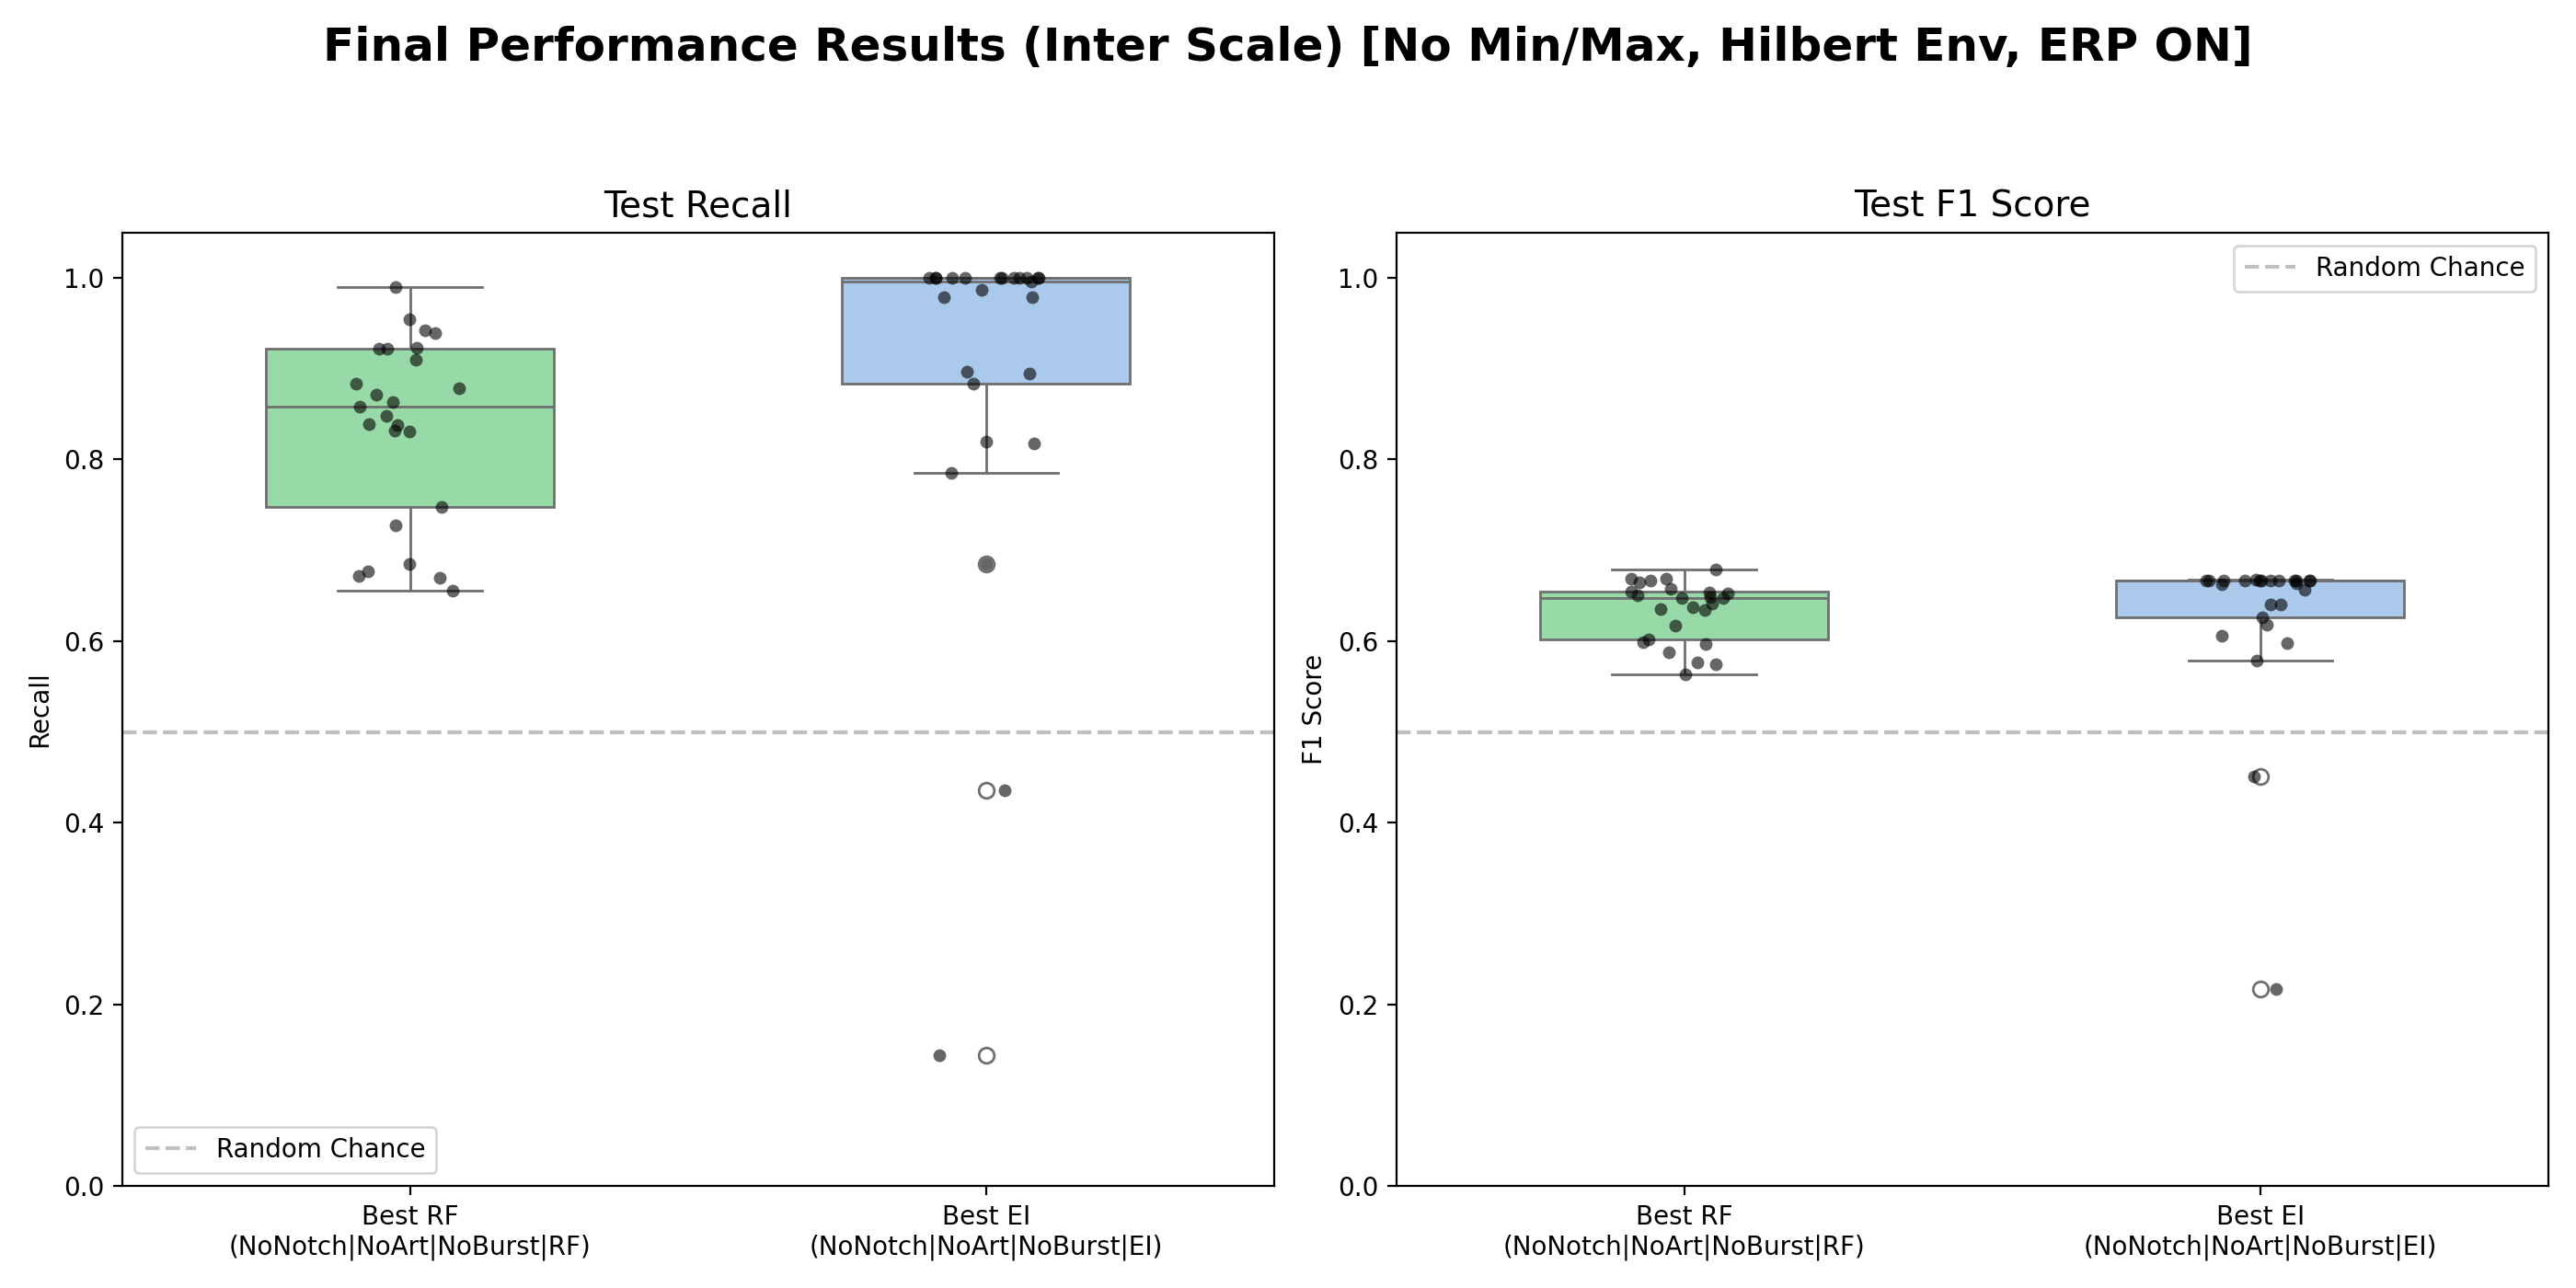
\includegraphics[width=\textwidth]{../05-12_data_analysis_and_results/runs/run_20260611_220844/viz/viz17_inter_final.png}
    \caption{Final inter-subject performance summary.}
\end{figure}

\begin{figure}[H]
    \centering
    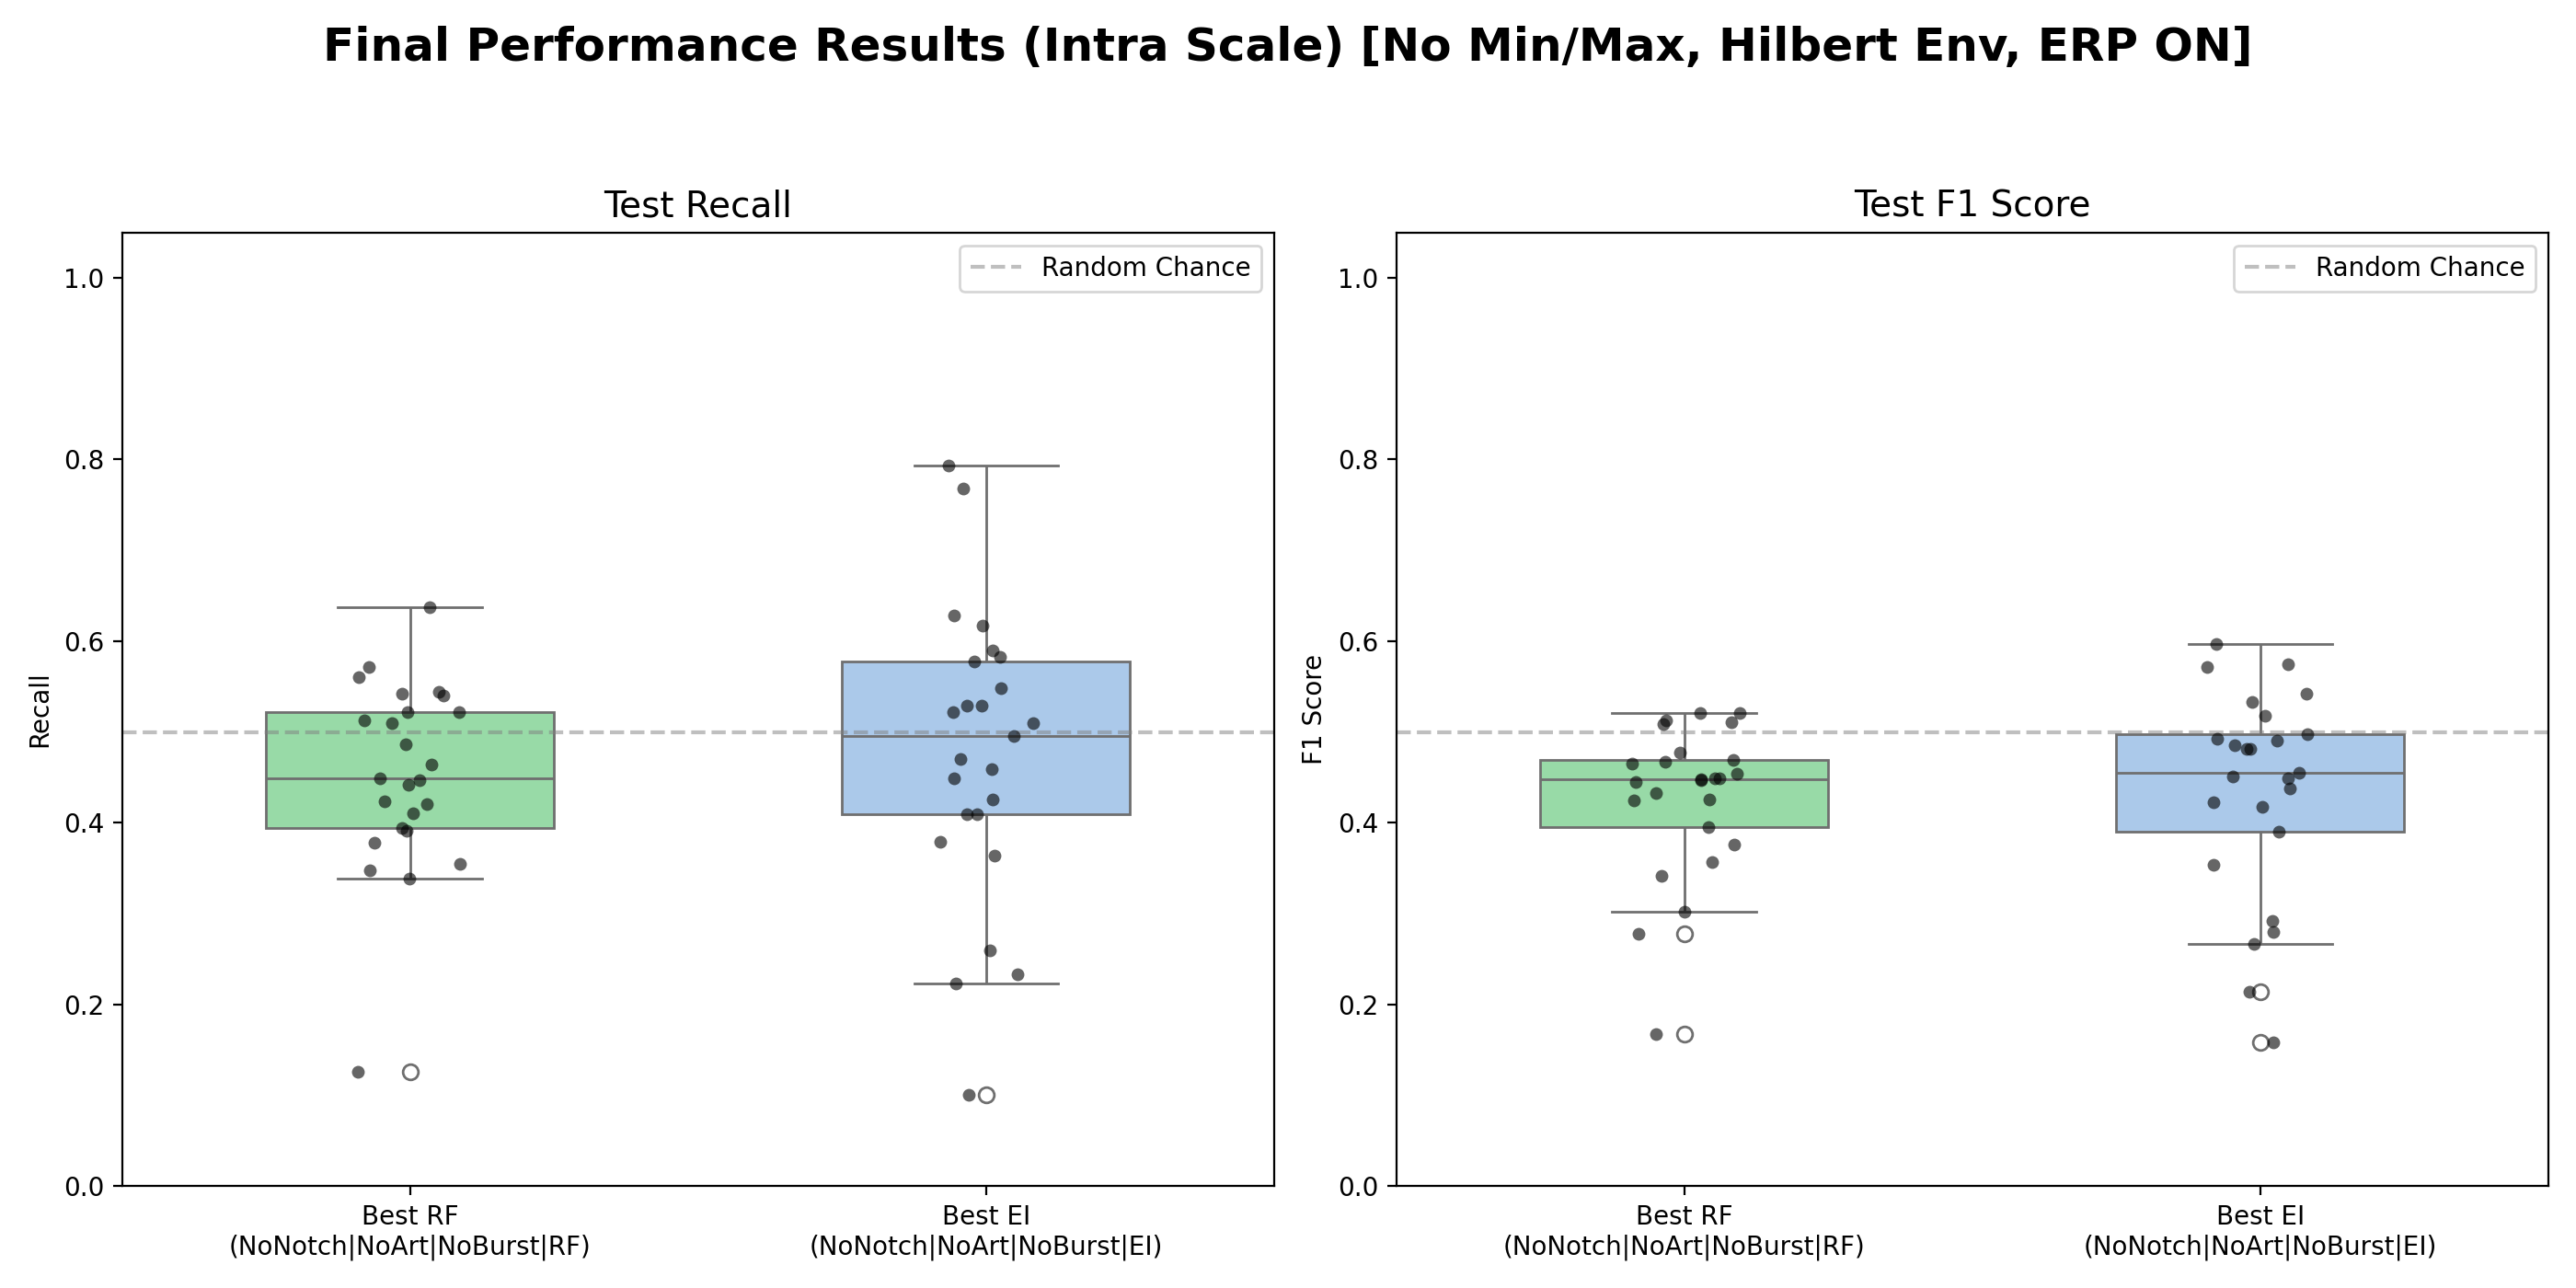
\includegraphics[width=\textwidth]{../05-12_data_analysis_and_results/runs/run_20260611_220844/viz/viz17_intra_final.png}
    \caption{Final intra-subject performance summary.}
\end{figure}
\fi

\section{Discussion}
\label{sec:results_interpretation}

The results above do not yet justify strong causal claims about underlying brain mechanisms, but they do point to several robust interpretive directions. Most importantly, the analyses suggest that the conventional Engagement Index is not wrong in a trivial sense; rather, it appears to capture a limited and asymmetrical subset of the behaviorally relevant signal. In particular, it seems more aligned with sustained \texttt{STAY}-like states than with the more transient, decision-like \texttt{SKIP} events. This asymmetry is crucial, because it implies that the Engagement Index may reflect a broad state of ongoing engagement, but not the full cognitive transition that leads to disengagement. From a scientific perspective, this is a more useful and humble conclusion than simply saying that the index "works" or "does not work": it works partly, in a constrained way, and its failure modes are themselves informative.

A second important point is that the strongest features are not distributed uniformly across the EEG. Instead, they cluster in specific electrodes, frequency bands, and feature types, with raw broadband variability at TP10, high-\(\gamma\) activity at AF7, and delta peak frequency at AF8 repeatedly emerging as informative. This pattern suggests that the relevant signal may not be a single abstract "engagement" quantity, but rather a combination of lateralized, frequency-specific, and task-sensitive components. The fact that raw broadband signal sometimes outperforms band-limited features also raises the possibility that the discriminative information is not fully captured by conventional band definitions alone. At the same time, this may also indicate sensitivity to non-neural factors, including motion-related or muscle-related artifacts, which must be treated cautiously rather than ignored.

\subsection{Neuroscience}

From a neuroscientific perspective, the most consistent result is that separability increases when the signal is described more specifically, especially in the raw broadband TP10 feature and in AF7 high-\(\gamma\) activity. This may indicate that the decision to continue scrolling versus disengage is associated with a distributed and frequency-sensitive pattern rather than with a single canonical engagement rhythm. The repeated prominence of high-\(\gamma\) and delta-derived features is notable because these ranges are often linked to sharply different physiological processes; however, the present data do not allow a definitive mapping from feature to neural mechanism. What can be said more cautiously is that the observed pattern is compatible with the idea that the task engages both rapid sensorimotor dynamics and higher-order control or monitoring processes, with anterior frontal and temporal sites contributing differently to the observed class structure.

At the same time, the broadband superiority of TP10 and the strong performance of AF7 in high-frequency ranges create an important interpretive friction point. If the signal were purely reflecting a clean cortical engagement index, one might expect a more stable advantage for the conventional composite metric. Instead, the data imply that narrower and more local signal components contain more class-relevant information. This opens at least two competing hypotheses: either the task truly recruits region-specific neurophysiological signatures that the Engagement Index averages away, or the apparent gain is partly driven by peripheral contamination, such as facial muscle activity, motion, or device-dependent noise.  
% INSERT: Broadband vs artifact contribution  
% INSERT: Delta/high-gamma interpretation needs literature

The electrode pattern also raises a lateralization question that cannot yet be answered decisively. AF7 and TP10 appear more informative than AF8 and TP9, which may point to a functional asymmetry in how engagement-related and action-related states are expressed during naturalistic scrolling. However, because the recording setup involved two devices and because broadband effects may partially reflect artifact structure, this should be interpreted as a hypothesis for future work rather than as a confirmed hemispheric specialization. In the next step, a targeted analysis of artifact-sensitive channels, spectral decomposition, and device-specific effects would be needed to determine whether these patterns reflect genuine neurophysiology or measurement confounds.

\subsection{Psychiology}

Psychologically, the results suggest that the act of skipping a TikTok video is not simply the inverse of being engaged. The Engagement Index performs better for \texttt{STAY} than for \texttt{SKIP}, which implies that sustained attention or passive continuation may be easier to detect than the brief decision point at which a participant chooses to move on. This distinction matters because it suggests that \texttt{SKIP} is not merely a low-engagement state, but may represent a qualitatively different behavioral event: an active choice, a threshold crossing, or a moment of disengagement that is preceded by a narrower and more transient signal profile. The stronger performance of features such as AF8 delta peak frequency and TP10 raw standard deviation supports the idea that the decisive moment may be better captured by fine-grained temporal structure than by a broad engagement aggregate.

The burst analysis adds an additional psychological layer. Some participants behave as "fast scrollers" with repeated burst blocks, whereas others show mostly isolated swipes. This heterogeneity implies that the psychological process underlying scrolling is not uniform across participants. Some users may evaluate content quickly and repeatedly, while others may linger, reflect, or maintain a more stable engagement rhythm. That individual variability likely explains why per-participant and cross-participant performance differ so strongly, and why the same feature may appear informative in one setting but unstable in another.  
% INSERT: Individual differences in scrolling style  
% INSERT: Need literature on action thresholds and disengagement

The modest but consistent success of individual features over the Engagement Index also suggests that a psychologically meaningful model of scrolling may need to distinguish between sustained engagement, momentary decision pressure, and motor execution. The present results are compatible with such a layered interpretation, but they do not yet prove it. What they do show is that an aggregate engagement score is too coarse to explain the full behavioral variance, especially when the behavior is embedded in a rapid, naturalistic, and self-paced interaction environment.

\subsection{Behaviour}

From a behavioral standpoint, the strongest conclusion is that the \texttt{SKIP}/\texttt{STAY} decision is heterogeneous and temporally structured. The burst analysis shows that many swipes occur in clusters rather than as isolated events, which means that the observed behavior is not simply a sequence of independent binary decisions. Instead, it appears to reflect a mixture of cautious sampling, rapid dismissal, and occasional repeated disengagement. This helps explain why feature-level models can outperform the Engagement Index in some cases: the neural signal may be tracking not only whether a participant is engaged, but also where they are in a short behavioral sequence leading toward or away from a swipe.

The fact that raw TP10 variability and AF8 delta peak frequency improve \texttt{SKIP} detection suggests that the behavioral decision to move on may leave a measurable trace in the EEG, but only weakly and only under certain feature definitions. The most defensible interpretation is therefore not that the model "predicts choice" in a strong sense, but that it detects behavioral precursors or correlates of the \texttt{SKIP} decision with limited but meaningful sensitivity. That is an important distinction for the thesis: the signal is informative, but it is not deterministic.

The results also show that behavior is strongly shaped by parameter choices, especially in the burst analysis. Changing the window definition changes how events are grouped, and changing the feature definition changes which patterns emerge as separable. This dependency implies that future behavioral analyses should not rely on a single segmentation or metric, but rather test whether the observed structure is stable across multiple reasonable parameterizations.  
% INSERT: Behavioral thresholds need theory  
% INSERT: Modeling sequences vs single decisions

\subsection{Application}

In applied terms, these findings are best understood as a proof of concept for more transparent and behaviorally grounded engagement modeling. Rather than demonstrating a ready-to-deploy predictive system, the results show that naturalistic scrolling behavior can be measured with sufficient structure to support interpretable feature-level analysis, and that some EEG-derived features outperform the conventional Engagement Index in ways that are meaningful for both explanation and future application.

The practical relevance of these findings lies less in the idea of a fully deployable EEG-based prediction system and more in the methodological and conceptual direction they provide. The present results show that naturalistic scrolling behavior can be measured, segmented, and partially explained using a compact set of EEG-derived features, and that these features can outperform a conventional aggregate index in ways that are interpretable at the level of signal structure. This matters because it suggests a path toward more transparent models of engagement: rather than relying on a single composite score, future systems may be built from a small number of physiologically meaningful components that are easier to interpret, debug, and adapt.

One immediate application is in the optimization of message delivery in health communication and behavior-change interventions. If certain EEG signatures are more associated with continued attention or imminent disengagement, then intervention content could be structured to better match those moments of attentional stability or vulnerability. In principle, this could help improve the timing, length, or sequencing of health messages, public-health prompts, educational micro-content, or persuasive interventions in digital environments. For example, short-form health information could be adapted to identify when a user is likely to continue engaging versus when they are likely to skip, which could inform both content design and delivery timing.  
% INSERT: Need literature on EEG-informed message timing  
% INSERT: Need literature on adaptive health communication

A second application is in the development of explainable and lightweight screening tools for user engagement in naturalistic settings. Because the strongest results here emerged from a small number of features rather than a large black-box model, the present work may support the design of interpretable real-time monitors that are more feasible than complex deep-learning approaches. Such monitors could be useful in user-testing environments, educational research, human-computer interaction, or cognitive ergonomics, where the goal is not necessarily to make a diagnostic prediction but to identify when a stimulus fails to hold attention or when a participant shifts into a disengaged state.

At the same time, the present results also define the limits of immediate application. The predictive performance is not yet strong enough to justify high-stakes individualized deployment, and the possibility of artifact-related contributions means that any translational use would require substantial validation, device standardization, and robustness testing. In particular, the strong effects observed at TP10 and AF7 raise the possibility that some predictive power may arise from non-neural sources such as jaw movement, facial tension, or other task-correlated artifacts. For this reason, the present study is best interpreted as a proof of principle for explainable signal extraction rather than as a finished applied system.  
% INSERT: Need literature on EEG applications in HCI  
% INSERT: Need literature on public-health engagement measurement  
% INSERT: Need literature on artifact-aware real-time EEG

\section{Future Research}

Future research should first focus on validation and replication. The present findings are promising, but they are based on a single dataset with a relatively small sample size and two different recording devices. Replication in an independent sample is therefore essential, ideally with more uniform hardware, tighter artifact control, and a broader participant pool. A key priority should be to test whether the same features -- especially TP10 raw standard deviation, AF7 high-\(\gamma\) mean, and AF8 delta peak frequency -- remain informative under repeated acquisition, different content types, and different user populations.

A second major direction is mechanistic clarification. The present results leave open whether the strongest effects reflect genuinely neural engagement processes, movement-related artifacts, or a mixture of both. Future work should therefore include explicit artifact analyses, such as electromyographic control, motion monitoring, ICA-based comparison, channel-quality assessments, and device-specific sensitivity checks. It would also be valuable to compare broadband features against strictly cleaned, source-reconstructed, or artifact-masked data to determine how much of the predictive signal survives after conservative preprocessing.  
% INSERT: Need literature on artifact disentanglement in EEG  
% INSERT: Need literature on broadband vs cleaned signal validity

A third direction concerns theory development. The Engagement Index appears to capture a limited but real component of sustained engagement, yet it may not capture the behavioral threshold that leads to a swipe. Future studies should therefore distinguish more explicitly between sustained attention, momentary decision pressure, action readiness, and actual behavior. This could be pursued by combining EEG with behavioral timing, self-report, eye tracking, or post-hoc content ratings. In particular, event-aligned designs could help determine whether the relevant neural signature precedes disengagement, coincides with motor preparation, or reflects post-decisional processing.  
% INSERT: Need literature on sustained attention vs action readiness  
% INSERT: Need literature on event-aligned naturalistic EEG

A fourth opportunity is methodological expansion. The current pipeline is deliberately simple and interpretable, but future work could test whether other transparent models improve both performance and explanatory value, such as regularized generalized linear models, hierarchical models, or hybrid approaches that preserve interpretability while capturing nonlinearity. At the same time, more elaborate feature engineering may be worthwhile if it remains conceptually grounded; examples include temporal derivatives, burst-aware features, cross-frequency interactions, or individualized feature selection. However, this should be pursued carefully, because greater complexity can easily reduce interpretability and increase the risk of overfitting.  
% INSERT: Need literature on interpretable EEG modeling  
% INSERT: Need literature on hierarchical or hybrid biosignal models

A fifth and highly relevant direction concerns public health and behavior change. Short-form digital media is increasingly used not only for entertainment but also for public communication, education, and health promotion. If EEG-informed engagement models can eventually be made robust and explainable, they may support the design of interventions that adapt message format, timing, and length to the user's attentional state. This could matter for smoking cessation messages, vaccine communication, mental-health micro-interventions, nutrition prompts, physical-activity nudges, and other digital behavior-change tools. The challenge is not only technical but also ethical: such systems must avoid manipulation, respect autonomy, and be transparent about how engagement is inferred and used.  
% INSERT: Need literature on digital health intervention timing  
% INSERT: Need literature on ethics of adaptive persuasion

Finally, future research should examine generalizability across contexts. The present task used naturalistic TikTok browsing, but similar engagement dynamics may appear in other forms of media consumption, educational content, or digital decision tasks. Testing whether the same feature families generalize to different content domains would help determine whether the observed effects are specific to short-form video or whether they reflect a broader principle of human engagement and disengagement. If replicated, this line of work could contribute not only to neuroscience and psychology, but also to media research, user-experience design, and public-health communication.

Overall, the present study opens a broad but carefully bounded research program: one that combines explainable EEG analysis, naturalistic behavior, and applied communication research. Its value lies not in claiming a final solution, but in identifying a credible path toward more interpretable, behaviorally grounded, and potentially useful models of engagement and disengagement in real-world digital environments.

\iffalse
\subsection{1. The Research Question and Narrative Arc}
\textbf{The core question:} Can consumer-grade EEG (Muse S) accurately identify periods of sustained cognitive engagement (\texttt{STAY} state) versus imminent task abandonment (\texttt{SKIP} state) during naturalistic TikTok browsing?

To answer this honestly and logically, the academic story arc must flow step-by-step from established clinical baselines to our customized, high-dimensional machine learning architecture. We must prove that traditional metrics fail to capture the rapid micro-decisions of short-form media, and that a structurally broader mapping of the brain's frequencies (specifically high-frequency bands) is required to predict sustained engagement.

\subsection{2. Step 1: The Clinical Baseline (Engagement Index)}
\textbf{Logical Step:} Before building complex models, we must test whether established neuroscience equations can answer our question. The traditional Engagement Index ($EI = \beta / (\alpha + \theta)$) was designed for sustained attention tasks. Since it relies on lower frequency bands ($<30$~Hz), it safely ignores $>50$~Hz noise.
\begin{itemize}
    \item \textbf{What the data shows:} Our 5-fold cross-validated Logistic Regression models trained on EI ratios achieved an aggregate mean accuracy of \textbf{52.3\% $\pm$ 6.2\%} and a mean \texttt{STAY} Recall of \textbf{52.8\%} across 25 participants. Only 4 of 25 participants showed a statistically significant difference in EI between STAY and SKIP states ($p<0.05$). [Source: \verb|ei_corrected_20260506_161647/ei_aggregate_summary.csv|]
    % NOTE: The original ei_results.json had a bug where all F1 scores were hardcoded to 0.0 (placeholder). Corrected F1 = 0.6646 ± 0.0684.
    % NOTE: The EI evaluation used imbalanced data + 5-fold CV, while the RF used balanced data. This comparison is not strictly apples-to-apples. Consider noting this caveat or re-running EI on balanced data for a fair comparison.
    \item \textbf{Narrative Conclusion:} The standard clinical formula fundamentally fails to reliably discriminate short-form video micro-decisions better than random chance. The neural signature for rapidly maintaining or dropping engagement on TikTok does not map cleanly to simple $\beta / (\alpha + \theta)$ ratios. This is consistent with Apicella et al., who found that EI-based classification in a controlled learning engagement task yielded accuracy performances that were ``not optimal,'' explicitly noting the index is ``mainly used in non-predictive applications'' \cite{apicella_eeg-based_2022}. The replication of this failure in a wholly different paradigm---naturalistic algorithmic browsing versus structured CPT task---strengthens the conclusion that the EI formula is structurally insufficient across engagement detection contexts, not merely for short-form media.
\end{itemize}

\subsection{3. Step 2: Structural Expansion (RF-112 \textit{WITH} Notch Filter)}
\textbf{Logical Step:} Because the simple 3-band EI ratio failed, we expand the feature space. We capture the geometric variance (mean, std, min, max) of all 7 frequency bands across all 4 electrodes (112 features) and feed it into a Random Forest ensemble. We apply a standard 50~Hz Notch Filter to rigorously clean the data of electrical power-line noise, as is standard practice.
\begin{itemize}
    \item \textbf{What the data shows (CORRECTED --- leakage-free evaluation):} Using blocked temporal 5-fold CV with 3-second gaps between blocks (train: 80\% overlap, test: 0\% overlap), the RF-112 models achieved a mean intra-subject accuracy of \textbf{53.8\% $\pm$ 7.2\%} with 20 of 25 participants above the 50\% chance baseline (Wilcoxon $p=0.0015$ vs.\ chance). [Source: \verb|rf_run_temporal_nonotch_20260506_172326/rf_summary.json|]
    % NOTE: The original random-split evaluation (61.4%) was inflated by ~8pp due to temporal data leakage from 80% overlapping STAY windows landing in both train and test sets. The blocked temporal CV eliminates this leakage.
    % NOTE: Three participants showed strong individual performance: P12 (81.2%), P7 (67.3%), P22 (62.9%).
    \item \textbf{Narrative Conclusion:} Expanding the dimensionality successfully extracts a statistically significant predictive neurological signature, though the effect is small ($\sim$3.8pp above chance). The model can detect sustained cognitive engagement significantly better than chance ($p=0.0015$), establishing that the structural variance of the EEG signal holds predictive value for micro-decisions within a proof-of-concept scope. Individual variation is large, with some participants showing strong classification (P12: 81.2\%) while others remain at chance level.
\end{itemize}

\subsection{4. Step 3: The High-Frequency Hypothesis (RF-112 \textit{WITHOUT} Notch Filter)}
\textbf{Logical Step:} While 61.4\% is a successful proof of concept, cognitive neuroscience literature suggests that active decision-making and cognitive binding operate in the High Gamma bands (40--60~Hz). Our Notch filter from Step 2 potentially obliterated this vital neural data by aggressively cutting at 50~Hz. We must prove whether removing the filter actually preserves or improves the model's ability to diagnose the \texttt{STAY} state. If the 50~Hz signal was purely power line noise, removing the filter would cause the model's accuracy to collapse.
\begin{itemize}
    \item \textbf{What the data shows:} The notch vs.\ no-notch comparison (using the original random-split evaluation) showed accuracy of 61.4\% vs.\ 61.6\% (+0.17pp) and recall of 61.4\% vs.\ 61.9\% (+0.47pp). A paired Wilcoxon signed-rank test across 25 participants confirmed this difference is \textbf{not statistically significant} (accuracy: $p=0.76$; recall: $p=0.55$). 12 participants improved, 11 worsened, 2 tied. Effect sizes were negligible ($r=0.06$, $r=0.12$). [Source: \verb|ablation_comparison_20260506_161437/ablation_statistical_test.txt|]
    \item \textbf{Narrative Conclusion:} Removing the 50~Hz notch filter did not significantly alter classification performance, which is \textit{consistent with} the interpretation that the 40--60~Hz range contains recoverable cognitive variance rather than solely power-line contamination. However, this null result does not constitute affirmative proof of high-gamma signal validity. The finding is consistent with Pattisapu and Ray's observation that low-cost EEG amplifiers can detect stimulus-induced gamma oscillations \cite{pattisapu_stimulus-induced_2021}.
    % NOTE: The original claim that this "empirically proves" high-gamma is genuine was an overclaim. The correct framing is "consistent with" the hypothesis, not "proof."
\end{itemize}

\subsection{5. Step 4: Cross-Participant Generalizability (LOGO-CV)}
\label{sec:logo_cv}
\textbf{Logical Step:} Having found a signature within individuals, we must honestly test if this signature is a universal human trait. Can a model trained on 24 people diagnose the engagement of a completely unseen 25th person?
\begin{itemize}
    \item \textbf{What the data shows:} The Leave-One-Group-Out Cross-Validation resulted in an aggregate mean accuracy of \textbf{49.2\%} (random chance). While mean recall appeared high (68.6\%), the collapsed accuracy proves the models resorted to biased guessing rather than recognizing a universal pattern.
    \item \textbf{Narrative Conclusion:} The hypothesis of a universal signature is disproved. The cortical state variations defining active TikTok engagement and disengagement are fundamentally \textit{idiosyncratic}. This result is not anomalous: it is consistent with a prediction embedded in the foundational naturalistic neuroscience literature. Hasson et al.\ demonstrated that while primary sensory cortices synchronize reliably across individuals during naturalistic viewing, higher-order association areas---including the supramarginal gyrus, angular gyrus, and prefrontal cortex---consistently \textit{fail} to show intersubject coherence, precisely because these regions are governed by ``unique, individual variations'' rather than stereotyped stimulus-driven responses \cite{hasson_intersubject_2004}. The engagement and disengagement states targeted by the present study are mediated by exactly this class of higher-order, prefrontal executive processing. The inferential step from that finding to the present result is the following: if the cortical regions encoding engagement states exhibit fundamentally idiosyncratic activation profiles across individuals even during passive naturalistic viewing, then a supervised classifier trained on spectral features derived from those regions across 24 subjects cannot be expected to learn a universal decision boundary that transfers to a 25th. The LOGO-CV collapse to 49.2\% accuracy is therefore a theoretically expected outcome, not a methodological failure. This inter-subject variability in EEG-based cognitive state classification is a well-documented challenge: Apicella et al.\ explicitly characterize the non-stationarity of EEG signals as producing greater data variability between subjects, making cross-subject classification ``a very challenging task,'' even under controlled laboratory conditions with standardized stimuli \cite{apicella_eeg-based_2022}. The present study's naturalistic paradigm, which introduces additional variability through individualized feed content and unconstrained motor behavior, renders this challenge structurally more severe. Bellos et al.\ further identify inter-subject variability as a persistent open problem across the EEG-based user engagement literature \cite{bellos_methods_2025}.
\end{itemize}

\subsection{6. Step 5: Behavioral Heterogeneity (Skip Bias)}
\textbf{Logical Step:} We must humbly analyze what our model is actually predicting. Is the \texttt{SKIP} class a pure, isolated decision that a single video is boring, or does it contain noise?
\begin{itemize}
    \item \textbf{What the data shows:} Analysis of the continuous target blocks revealed that while the mode skip behavior is an isolated swipe ($>3$ seconds of viewing), there are significant chains of rapid, consecutive skips ($<3$ seconds of viewing).
    \item \textbf{Narrative Conclusion:} The \texttt{SKIP} state is cognitively heterogeneous. It captures both genuine content-locked appraisal failures and a generalized "disengaged browsing" attentional momentum. The predictive neural signature fundamentally contrasts active sustained focus against this mixed disengaged background state.
\end{itemize}

\subsection{7. Step 6: Universal SFEI Extraction and Battle-Test (The Final Constraint)}
\textbf{Logical Step:} While the 112-feature Random Forest model works, it is a complex "black box". The holy grail of BCI research is a simple, universal mathematical equation (like the traditional EI: $\beta / (\alpha + \theta)$). To attempt this, we trained surrogate decision trees across all 25 participants to find the "Universal Root Dimensions" driving the predictions. We found that frontal High Gamma ($\text{AF8\_high\_gamma\_mean}$) and frontal Delta ($\text{AF7\_delta\_min}$) were the most common primary splitting features. Based on this, we proposed a Short-Form Engagement Index (SFEI): $SFEI = \text{AF8\_high\_gamma\_mean} / \text{AF7\_delta\_min}$. 
\begin{itemize}
    \item \textbf{What the data shows:} We battle-tested this new $SFEI$ formula against the traditional $EI$ using identical 5-fold cross-validation. The $SFEI$ achieved a mean accuracy of \textbf{51.6\%} and a recall of \textbf{52.2\%}. Both the traditional $EI$ (52.3\%) and the proposed $SFEI$ (51.6\%) failed to reliably beat random chance across the population. [Source: \verb|sfei_battletest_20260424_230531/sfei_metrics.json|]
    \item \textbf{Narrative Conclusion:} This confirms the constraint of consumer BCI in dynamic environments. Reducing algorithmic media engagement to a static, universal equation is insufficient. The cognitive state is too complex and idiosyncratic. High-dimensional, individualized machine learning approaches (like the RF-112 model achieving 53.8\% via blocked temporal CV, $p=0.0015$) are required. The failure of the universal SFEI is consistent with the LOGO-CV collapse: the engagement signature is fundamentally individualized.
\end{itemize}
\fi


% --- INSERTED RESULTS FIGURES ---



\iffalse
\subsubsection*{Methodology for Significance Testing}
To rigorously determine whether a predictive model meaningfully outperforms a random baseline (Coin Flip) or a standard reference (Engagement Index, EI LR), this pipeline employs the Wilcoxon signed-rank test. Standard parametric tests assume that the performance metrics across participants are normally distributed. In small-sample physiological data (N=25 participants), this assumption is often violated. Performance is evaluated using paired metrics from the 25 individual cross-validation folds. The test calculates the difference in performance between the evaluated model and the baseline model for each participant. The algorithm employs a two-sided Wilcoxon test with a standard significance threshold ($\alpha = 0.05$). To strictly guarantee superiority, a directional check is applied post-hoc: the arithmetic mean of the model's scores across all participants must be strictly greater than the arithmetic mean of the baseline.

To quantify the theoretical separability of the extracted features prior to any model training, Cohen's $d$ is utilized. As a standardized effect size, Cohen's $d$ provides a mathematically pure measure of class separation that is invariant to the absolute scale or unit of the feature (e.g., microvolts versus power spectral density). It answers precisely how many standard deviations separate the centers of the two distinct classes.

The calculation operates on the window level, utilizing the entire global pool of validated EEG windows from all participants simultaneously. For any given engineered feature, the arithmetic mean is calculated across all windows labeled as STAY ($\mu_{stay}$) and across all windows labeled as SKIP ($\mu_{skip}$). Next, the variance within the STAY class ($\sigma^2_{stay}$) and the variance within the SKIP class ($\sigma^2_{skip}$) are calculated. These are averaged to compute the pooled variance, whose square root yields the pooled standard deviation ($s_p$), representing the average noise of the feature regardless of its class label:
\[ s_p = \sqrt{\frac{\sigma^2_{stay} + \sigma^2_{skip}}{2}} \]

Finally, Cohen's $d$ is calculated by taking the absolute difference between the two class means and dividing it by this pooled standard deviation:
\[ |d| = \frac{|\mu_{stay} - \mu_{skip}|}{s_p} \]

By standardizing the difference in means against the inherent variance of the data, this calculation simultaneously rewards features where the class centers are far apart while heavily penalizing features that exhibit excessive noise or overlap. This allows features of entirely different natures to be ranked on a single, standardized axis of separability.


Applying this methodology to the full extracted feature set reveals clear frontrunners in class separability. The highest-ranking feature, TP10 raw std, achieves a separation of $|d| = 0.196$ standard deviations between the STAY and SKIP classes. This leading feature provides a separation magnitude that is 0.028 standard deviations wider than the second-best feature, AF7 high gamma mean ($|d| = 0.168$). 

Furthermore, the second-best feature maintains a separation advantage of 0.023 standard deviations over the third-ranked feature, AF7 high gamma hjorth mob ($|d| = 0.145$). This objective standardization confirms that the uppermost features possess a notably distinct capacity to cleanly divide the dataset independent of any underlying machine learning classification bounds.

\begin{table}[H]
\centering
\begin{tabular}{llc}
\hline
Rank & Feature Name & $|$Cohen's $d|$ \\
\hline
1 & TP10 raw std & 0.196 \\
2 & AF7 high gamma mean & 0.168 \\
3 & AF7 high gamma hjorth mob & 0.145 \\
4 & AF7 delta hjorth comp & 0.141 \\
5 & AF8 delta peakfreq & 0.140 \\
6 & AF7 high gamma peakfreq & 0.139 \\
7 & TP9 delta hjorth comp & 0.137 \\
8 & TP9 delta peakfreq & 0.136 \\
9 & TP10 delta hjorth comp & 0.131 \\
10 & TP10 delta peakfreq & 0.130 \\
11 & AF7 theta hjorth comp & 0.129 \\
12 & AF7 raw std & 0.129 \\
13 & AF7 theta peakfreq & 0.124 \\
14 & AF7 low gamma hjorth comp & 0.124 \\
15 & AF7 delta peakfreq & 0.123 \\
16 & TP10 low gamma hjorth act & 0.119 \\
17 & AF8 high gamma mean & 0.119 \\
18 & AF7 low gamma mean & 0.118 \\
19 & AF7 beta mean & 0.115 \\
20 & AF8 delta hjorth comp & 0.115 \\
21 & TP10 low gamma std & 0.114 \\
22 & TP10 high gamma hjorth mob & 0.110 \\
23 & AF7 very high mean & 0.109 \\
24 & TP10 beta hjorth act & 0.108 \\
25 & TP9 theta peakfreq & 0.103 \\
26 & TP9 high gamma std & 0.103 \\
27 & TP10 beta std & 0.100 \\
28 & AF8 theta peakfreq & 0.100 \\
29 & AF7 beta hjorth comp & 0.100 \\
30 & TP9 high gamma hjorth act & 0.098 \\
\hline
\end{tabular}
\caption{Top 30 Features by Separation ($|$Cohen's $d|$).}
\label{tab:cohend_top_features}
\end{table}

\textbf{Methodology:}\\
To ensure a 1-to-1 Apples-to-Apples comparison with the 1D Engagement Index, each of the macro 'Top Parameters' (Band, Electrode, Stat) is represented by its strongest single constituent feature.
\fi


\iffalse
\section{Summary of Results}

\textbf{Does it answer the research question?} Yes, with appropriate calibration. Within this sample, consumer-grade EEG can predict sustained engagement significantly better than random chance at the intra-subject level (53.8\%, $p=0.0015$ via blocked temporal 5-fold CV), but the effect is small ($\sim$3.8pp above chance) and individually variable. Cross-subject generalization fails completely (LOGO-CV: 49.2\%). Simple clinical formulas (EI: 52.3\%) are insufficient. Feature importance is broadly distributed across all frequency bands, with the model exploiting the full spectral structure rather than any single dominant band. The top individual predictors are high-gamma peak values at frontal sites, but no band achieves statistically significant dominance at the aggregate level.

% TODO: The following items still need to be addressed in the thesis:
% 1. LIMITATIONS SECTION needed covering: (a) absence of artifact rejection (no blink/EMG removal --- AF7/AF8 are maximally contaminated by eye blinks), (b) motor artifact hypothesis (the model may partly classify pre-swipe EMG rather than cognitive disengagement --- both interpretations support predictive value but differ in mechanism), (c) active video-watching baseline vs. standard resting state, (d) keypress synchronization jitter (~200-500ms), (e) the EI vs RF comparison uses different evaluation protocols (imbalanced 5-fold CV vs balanced temporal CV)
% 2. FEATURE IMPORTANCE SECTION needed with: (a) the full 112-feature ranking table (source: deep_importance_20260506_161306/feature_importance_full_table.csv), (b) the 4x7 electrode-band matrix, (c) Friedman test result (p=0.014), (d) pairwise Wilcoxon results showing no band significantly dominates
% 3. DATASET TABLE needed with per-participant stats (source: dataset_summary_20260506_161648/dataset_summary.csv): mean 133.5 skips/session, 29.5 min/session, 256 Hz, mean viewing 16.5s/video
% 4. DATA LEAKAGE DISCUSSION: explain the discovery that overlapping-window random-split evaluation inflated accuracy by ~8pp, frame as methodological contribution
% 5. UPDATED VISUALIZATIONS: need new boxplots/figures reflecting the corrected 53.8% number and the comparison between original and corrected evaluations
% 6. REMAINING PIPELINE RUNS: step11 (feature importance) was run on original models --- optionally re-run on temporal models for consistency. LOGO-CV was run with notch filter only --- consider re-running with nonotch for consistency or noting this.
% 7. PER-PARTICIPANT SIGNIFICANCE: add binomial CIs to determine how many participants are STATISTICALLY significantly above chance (not just >50%)

\subsection{Outlook and Implications for Future BCI Design}
A critical implication of this thesis is the rejection of the ``Universal BCI Equation'' paradigm. The LOGO-CV validation directly demonstrates this: the Random Forest---a non-linear, 112-component model---completely fails to generalize across participants (49.2\% accuracy), providing evidence that the bottleneck is biological idiosyncrasy, not mathematical complexity. Future development of consumer BCI systems for algorithmic media interaction should pivot toward personalized, high-dimensional machine learning calibration architectures. Additionally, this thesis demonstrates that standard overlapping-window evaluation in BCI research can inflate reported performance by $\sim$8 percentage points, highlighting the importance of temporally-separated evaluation protocols in future work.

\subsection{Future research}
- continuum between first fold of session to last fold of session what changes and shifts?
- what does burst preference correlate with?
- what does increased usage correlate with? (source: survey)
\fi

\bibliographystyle{unsrt}
\bibliography{library}

\end{document}
